% cute-zhihu.tex — CuTe 知乎优秀文章合集（reed & 竹熙佳处）
% 构建：cd book/cute-zhihu/ && TEXMFCNF=../../tex: xelatex -interaction=nonstopmode cute-zhihu.tex（×2）
\documentclass[9pt,openany]{ctexbook}
% preamble.tex — LeetCUDA 技术书导言
% 抽取自 tex/notes-v2.tex（8 色调色板/字体/lstset），ctexart → ctexbook
% RFC-0.2 / RFC-0.4 关键字表已审计（2026-09-11，grep 全源码验证）

\usepackage[paperwidth=210mm,paperheight=297mm,left=1.35cm,right=1.35cm,top=1.4cm,bottom=1.6cm]{geometry}
\usepackage{listings,xcolor,fancyhdr}
\usepackage{graphicx}
\usepackage{needspace}
\usepackage{amsmath,amssymb}
\usepackage{amsthm}
\usepackage{booktabs}
\usepackage{longtable}
\usepackage{enumitem}
\usepackage{tikz}
\usetikzlibrary{matrix,positioning,patterns,arrows.meta,shapes,calc,fit}
\usepackage{subcaption}
\usepackage{array}
\usepackage{adjustbox}

% 长行内代码（\texttt 标识符/路径）混排中文时的断行弹性，压制 Overfull \hbox
\emergencystretch=2em

\pagestyle{fancy}
\fancyhf{}
\fancyhead[LE]{\scriptsize\leavevmode\leftmark}
\fancyhead[RO]{\scriptsize\leavevmode\rightmark}
\fancyfoot[C]{\scriptsize \thepage}
\renewcommand{\headrulewidth}{0.4pt}
\renewcommand{\footrulewidth}{0pt}

% --- 8 色调色板（VSC 风格，同 notes-v2.tex） ---
\definecolor{vscBackground}{RGB}{248,248,248}
\definecolor{vscText}{RGB}{31,35,40}
\definecolor{vscLineNumber}{RGB}{142,142,142}
\definecolor{vscKeyword}{RGB}{0,90,158}

% TikZ 语义色板（2026-09-20：全图统一着色，替代纯灰度）
% 用法：填充大面积用 tkFill* 浅色系，边框/文字/箭头用主色系；无语义的中性结构可保留灰度
\definecolor{tkBlue}{RGB}{33,113,181}     % 结构/主数据/流水
\definecolor{tkGreen}{RGB}{53,141,106}    % 修复/after/有效/命中
\definecolor{tkOrange}{RGB}{216,130,28}   % 冲突/before/警示过渡
\definecolor{tkRed}{RGB}{203,54,47}       % 错误/溢出/坏例
\definecolor{tkPurple}{RGB}{122,82,158}   % 次要强调/对照
\definecolor{tkFillBlue}{RGB}{232,241,250}
\definecolor{tkFillGreen}{RGB}{230,243,236}
\definecolor{tkFillOrange}{RGB}{252,240,224}
\definecolor{tkFillRed}{RGB}{251,233,231}
\definecolor{tkFillPurple}{RGB}{240,234,247}

% CuTe/GEMM layout 图 8 色 hue 环（cute_gemm 风格：hue=tile 身份，intensity=tile 内位置）
% 与 colfax/cf-macros.tex 保持一致；用法：fill=colorxN!10..!60
\definecolor{colorx1}{RGB}{255,0,0}      % Red
\definecolor{colorx2}{RGB}{255,191,0}    % Orange-yellow
\definecolor{colorx3}{RGB}{128,255,0}    % Yellow-green
\definecolor{colorx4}{RGB}{0,255,128}    % Green-cyan
\definecolor{colorx5}{RGB}{0,255,255}    % Cyan
\definecolor{colorx6}{RGB}{0,128,255}    % Blue
\definecolor{colorx7}{RGB}{128,0,255}    % Indigo
\definecolor{colorx8}{RGB}{255,0,255}    % Magenta
\definecolor{vscComment}{RGB}{0,128,0}
\definecolor{vscAccent}{RGB}{163,21,21}
\definecolor{vscEmphasis}{RGB}{43,145,175}
\definecolor{vscFrame}{RGB}{210,210,210}

\setmonofont{DejaVu Sans Mono}
\setCJKmonofont{Noto Sans Mono CJK SC}

% --- 定理类环境 ---
\newtheorem{theorem}{定理}[chapter]
\newtheorem{lemma}[theorem]{引理}
\theoremstyle{definition}
\newtheorem{definition}[theorem]{定义}
\theoremstyle{remark}
\newtheorem*{remark}{注记}
% 勘误与考据框注（源码注释核查结果，全量记录在 book/CHECKLOG.md）
\newtheoremstyle{kaowustyle}{6pt}{6pt}{\small}{}{\bfseries}{：}{ }{}
\theoremstyle{kaowustyle}
\newtheorem{kaogu}{实践经验}[chapter]

% --- 伪代码清单（E2 修复）：同框灰底，自动行号，# 注释 ---
\lstdefinestyle{pseudo}{
  language=, numbers=left, numberstyle=\scriptsize\color{vscLineNumber},
  basicstyle=\footnotesize\ttfamily\color{vscText},
  comment=[l]{\#}, commentstyle=\color{vscComment},
  keywordstyle=\bfseries\color{vscKeyword},
  morekeywords={function,for,to,do,end,if,then,else,while,return,in,parallel,foreach},
  backgroundcolor=\color{vscBackground}, frame=single, framerule=0.8pt,
  rulecolor=\color{vscFrame}, framesep=6pt, xleftmargin=4pt, xrightmargin=4pt,
  breaklines=true, columns=fullflexible, keepspaces=true, tabsize=2,
  aboveskip=4pt, belowskip=4pt, showstringspaces=false, upquote=true,
}
% --- 终端/测试输出清单（E6 修复）：无行号灰底框 ---
\lstdefinestyle{console}{
  language=, numbers=none,
  basicstyle=\footnotesize\ttfamily\color{vscText},
  backgroundcolor=\color{vscBackground}, frame=single, framerule=0.8pt,
  rulecolor=\color{vscFrame}, framesep=6pt, xleftmargin=4pt, xrightmargin=4pt,
  breaklines=true, columns=fullflexible, keepspaces=true, tabsize=2,
  aboveskip=4pt, belowskip=4pt, showstringspaces=false, upquote=true,
}

% --- 代码清单：firstnumber=auto（行号与源文件一致） ---
\lstset{
  language=C,
  basicstyle=\footnotesize\ttfamily\color{vscText},
  numbers=left,
  numberstyle=\scriptsize\color{vscLineNumber},
  numbersep=6pt,
  showstringspaces=false,
  breaklines=true,
  breakatwhitespace=false,
  tabsize=2,
  extendedchars=true,
  upquote=true,
  columns=fullflexible,
  keepspaces=true,
  backgroundcolor=\color{vscBackground},
  frame=single,
  framerule=0.8pt,
  rulecolor=\color{vscFrame},
  framesep=6pt,
  xleftmargin=4pt,
  xrightmargin=4pt,
  aboveskip=4pt,
  belowskip=4pt,
  firstnumber=auto,
  keywordstyle=\bfseries\color{vscKeyword},
  commentstyle=\color{vscComment},
  identifierstyle=\color{vscText},
  stringstyle=\color{vscAccent},
  morekeywords={__global__,__device__,__host__,__shared__,
    __constant__,__forceinline__,__align__,__restrict__,
    __syncthreads,threadIdx,blockIdx,blockDim,gridDim,
    warpSize,__shfl_sync,__shfl_xor_sync,atomicAdd,
    __float2half,half,half2,float2,float4,int4,uint32_t,
    cuda::barrier,CUtensorMap,constexpr,__expf,
    __fdividef,__fmaf_rn,__float22half2_rn,__half22float2,
    cudaMalloc,cudaFree,cudaMemcpy,cudaMemset,
    cudaDeviceSynchronize,cudaGetLastError,cudaGetErrorString,
    cudaEventCreate,cudaEventDestroy,cudaEventRecord,
    cudaEventElapsedTime,cudaEventSynchronize,
    cudaFuncSetAttribute,cudaFuncAttributeMaxDynamicSharedMemorySize,
    cudaMemcpyHostToDevice,cudaMemcpyDeviceToHost,cudaSuccess,
    cublasCreate,cublasDestroy,cublasSgemm,cublasGemmEx,cublasHgemm,
    cublasSetMathMode,cublasHandle_t,
    CUBLAS_OP_N,CUBLAS_OP_T,CUDA_R_16F,
    CUBLAS_COMPUTE_16F,CUBLAS_GEMM_DEFAULT,
    CUBLAS_GEMM_DEFAULT_TENSOR_OP,CUBLAS_TENSOR_OP_MATH,
    cuInit,cuTensorMapEncodeTiled,CUresult,CUDA_SUCCESS,
    CU_TENSOR_MAP_DATA_TYPE_FLOAT16,
    CU_TENSOR_MAP_INTERLEAVE_NONE,CU_TENSOR_MAP_SWIZZLE_128B,
    CU_TENSOR_MAP_L2_PROMOTION_NONE,CU_TENSOR_MAP_FLOAT_OOB_FILL_NONE,
    cuda::thread_scope_block,
    cuda::device::barrier_arrive_tx,
    cuda::device::experimental::cp_async_bulk_tensor_2d_global_to_shared,
    cuda::device::experimental::fence_proxy_async_shared_cta,
    __launch_bounds__,__cvta_generic_to_shared,
    allocate_and_create_tensor_map,create_tensor_map,
  },
  morekeywords=[2]{
    % 归约/elementwise/norm（base.cuh，2026-09-11 grep 验证）
    warp_reduce_sum,warp_reduce_max,block_reduce_sum,block_reduce_max,
    block_reduce_all,dot,dot_vec4,
    relu,relu_vec4,elementwise_add,elementwise_add_vec4,histogram,
    softmax_per_token,safe_softmax_per_token,online_safe_softmax_per_token,
    rms_norm,rms_norm_vec4,layer_norm,layer_norm_vec4,
    rope,mat_transpose,mat_transpose_padded,merge_attn_states,
    % GEMM 家族（sgemv/sgemm/hgemm.cuh）
    sgemv_k32,sgemv_k128,sgemv_k16,
    sgemm,sgemm_vec4,sgemm_tf32,f32x4_tf32x4_kernel,
    hgemm_mma_stages_tn,hgemm_mma_stages_tn_swizzle,
    hgemm_mma_stages_tn_cute,launch_hgemm_mma_stages_tn_cute,
    hgemm_wgmma_stages_tn,hgemm_tma_mma_ws_tn,
    % FlashAttention 家族（flash_attn.cuh）
    flash_attn_mma_stages_split_q,
    flash_attn_tma_mma_ws_stages_split_q,
    flash_attn_3_tma_ws_stages_split_q,
    flash_attn_mma_stages_split_q_cute,
    flash_attn_tma_mma_ws_split_q_cute,
    flash_attn_3_tma_mma_ws_split_q_cute,
    flash_attn_3_cute_tma_copy_smoke,
    fa_cute,FlashAttn2CuTeTraits,FlashAttn3CuTeTraits,
    % FFPA（ffpa_attn.cuh）
    FFPAAttnSplitDCuTeTraits,ffpa_split_d_cute,
    ffpa_attn_tma_mma_ws_split_d_cute,
    % 辅助
    fill_2D_regs,fill_3D_regs,div_ceil,make_smem_desc,test_hgemm_cute,
    expf,fmaxf,sinf,cosf,powf,sqrtf,rsqrtf,
    __shfl_sync,__shfl_xor_sync,lane_id,warp_id,
    block_row_max,block_row_max_new,block_row_sum,block_row_sum_new,
    CP_ASYNC_CG,CP_ASYNC_COMMIT_GROUP,CP_ASYNC_WAIT_GROUP,CP_ASYNC_WAIT_ALL,
    LDMATRIX_X4,LDMATRIX_X2,LDMATRIX_X2_T,HMMA16816,
    WGMMA_FENCE,WGMMA_COMMIT_GROUP,WGMMA_WAIT_GROUP,
    WGMMA_M64N128K16_F16F16F16,SMEM_DESC_ENCODE,
    FLOAT4,INT4,HALF2,
    % CuTe 标识符
    make_tensor,make_gmem_ptr,make_smem_ptr,make_shape,make_stride,
    make_coord,make_tile,make_layout,make_tensor_like,
    local_tile,tile_to_shape,composition,compose,
    TiledMMA,MMA_Atom,MMA_Traits,mma_traits,MMA_EU_RepeatT,MMA_P_T,
    SM80_16x8x16_F16F16F16F16_TN,SM80_CP_ASYNC_CACHEGLOBAL,
    SM75_U32x4_LDSM_N,UniversalCopy,
    Swizzle,Copy_Atom,Copy_Traits,copy_op,copy_traits,copy_atom,
    make_tiled_copy,make_tiled_copy_A,make_tiled_copy_B,make_tiled_copy_C,
    make_tiled_mma,
    get_slice,get_thread_slice,get,
    partition_S,partition_D,partition_fragment_A,partition_fragment_B,partition_fragment_C,
    retile_D,retile_S,
    copy,gemm,gemm_ss,gemm_rs,convert_layout_acc_rowcol,
    cp_async_fence,cp_async_wait,
    group_modes,size,cosize,clear,data,
    Int,Shape,Stride,Step,Coord,Tile,Layout,
    Underscore,LayoutLeft,LayoutRight,SwizzleBMS,
    swizzle_v1_impl,swizzle_v2_impl,
    SmemLayoutA,SmemLayoutB,SmemLayoutC,SmemLayoutAtom,SmemLayoutAtomC,
    G2SCopyA,G2SCopyB,S2GCopyC,S2RCopyAtomA,S2RCopyAtomB,R2SCopyAtomC,S2GCopyAtomC,
    g2s_tiled_copy_a,g2s_tiled_copy_b,s2r_tiled_copy_a,s2r_tiled_copy_b,
    r2s_tiled_copy_c,s2g_tiled_copy_c,
    thr_mma,tiled_mma,tCrA,tCrB,tCrD,tCrC_r2s,tCsC_r2s,tCsC_s2g,tCgC_s2g,
    tensor,layout,TensorMap,
  },
  keywordstyle=[2]\bfseries\color{vscEmphasis},
  morekeywords=[3]{
    NOTES_V2_ENABLE_CUDNN,NOTES_V2_ENABLE_CUTE,NOTES_V2_ENABLE_SETMAXNREGS,
    NOTES_V2_ENABLE_SWIZZLE_V2,NOTES_V2_ENABLE_TMA_MMA_WS,NOTES_V2_ENABLE_WGMMA,
    NOTES_V2_REG_ALLOC,NOTES_V2_REG_DEALLOC,
    mbarrier_init,mbarrier_arrive_expect_tx,mbarrier_wait,
  },
  keywordstyle=[3]\bfseries\color{vscAccent},
}

% CuTe 白皮书导读（ch19b）专用代码环境
\lstnewenvironment{python}{%
  \lstset{style=console,language=Python,tabsize=4,
    keywordstyle=\bfseries\color{vscKeyword},
    commentstyle=\color{vscComment},
    stringstyle=\color{vscAccent}}}{}
\lstnewenvironment{cpp}{%
  \lstset{style=console,language=C++,tabsize=2,
    keywordstyle=\bfseries\color{vscKeyword},
    commentstyle=\color{vscComment},
    stringstyle=\color{vscAccent}}}{}

\usepackage[unicode,bookmarksnumbered,colorlinks,linkcolor=vscKeyword,citecolor=vscKeyword,urlcolor=vscEmphasis]{hyperref}
\usepackage{xurl}
\usepackage{float}
\usepackage{placeins}

\title{CuTe 知乎文章合集\\{\large reed \& 竹熙佳处系列文章忠实整理}}
\author{整理：LeetCUDA Project}
\date{2026 年 9 月}

\begin{document}

% ============ 封面（首页声明） ============
\begin{titlepage}
  \centering
  \vspace*{3cm}
  {\Huge\bfseries CuTe 知乎文章合集}\\[1.2em]
  {\Large reed \& 竹熙佳处 优秀 CuTe 系列文章忠实整理}\\[4em]
  \fbox{\parbox{0.88\textwidth}{\centering
    {\Large\bfseries 郑重声明}\\[1em]
    {\large
    本书仅对知乎作者 \textbf{reed}（专栏「CUDA高性能编程」）与 \textbf{竹熙佳处}
    （CuTe 教程系列）两位作者的 CuTe 系列优秀文章进行\textbf{忠实整理，不对原文内容做任何修改}。}\\[0.8em]
    {\large 本书\textbf{仅用于开源学习}，\textbf{不得用于任何商业用途}。}\\[0.8em]
    {\normalsize 全部文章著作权归原作者所有，转载请注明原文出处。}
  }}\\[4em]
  {\large 2026 年 9 月}
  \vfill
\end{titlepage}

% ============ 前言 ============
\chapter*{整理说明}
\addcontentsline{toc}{chapter}{整理说明}

本书系统整理了知乎作者 \textbf{reed}（专栏「CUDA高性能编程」）与 \textbf{竹熙佳处}
两位作者的 CuTe（CUTLASS 3.x 张量抽象）系列文章，共 20 篇，按系列依赖/发表顺序编排。
整理过程中\textbf{忠实保留原文内容与图片，不做任何修改}；仅做 Markdown 到 \LaTeX{}
的排版映射（标题层级、代码块、公式、图片位置与图注均与原文一致）。

全部文章于 2026-09-20 自知乎原文页面抓取，共 109 幅原图。两作者文章分别成篇（Part），
每章章首标注作者与原文链接，便于溯源。

本书仅用于开源学习，不得用于任何商业用途。

\section*{reed 系列文章来源（13 篇）}
\begingroup\small
\begin{tabular}{@{}c>{\raggedright\arraybackslash}p{0.78\textwidth}@{}}
  \toprule
  章节 & 原文 \\
  \midrule
  01 & cute 之 Layout\newline\url{https://zhuanlan.zhihu.com/p/661182311} \\
  02 & cute Layout 的代数和几何解释\newline\url{https://zhuanlan.zhihu.com/p/662089556} \\
  03 & cute 之 Tensor\newline\url{https://zhuanlan.zhihu.com/p/663093816} \\
  04 & cute 之 Copy抽象\newline\url{https://zhuanlan.zhihu.com/p/666232173} \\
  05 & cute 之 MMA抽象\newline\url{https://zhuanlan.zhihu.com/p/663092747} \\
  06 & cute 之 Swizzle\newline\url{https://zhuanlan.zhihu.com/p/671419093} \\
  07 & cute 之 Hopper前言\newline\url{https://zhuanlan.zhihu.com/p/1948048832794427610} \\
  08 & cute 之 Hopper MBarrier\newline\url{https://zhuanlan.zhihu.com/p/1962636004235153810} \\
  09 & cute 之 Hopper TMA\newline\url{https://zhuanlan.zhihu.com/p/1985678344352731952} \\
  10 & cute 之 TMA Descriptor编码与隐藏的第21bit\newline\url{https://zhuanlan.zhihu.com/p/2037200219700449995} \\
  11 & cute 之 简单GEMM实现\newline\url{https://zhuanlan.zhihu.com/p/667521327} \\
  12 & cute 之 GEMM流水线\newline\url{https://zhuanlan.zhihu.com/p/665082713} \\
  13 & cute 之 高效GEMM实现\newline\url{https://zhuanlan.zhihu.com/p/675308830} \\
  \bottomrule
\end{tabular}
\endgroup

\section*{竹熙佳处系列文章来源（7 篇）}
\begingroup\small
\begin{tabular}{@{}c>{\raggedright\arraybackslash}p{0.78\textwidth}@{}}
  \toprule
  章节 & 原文 \\
  \midrule
  01 & 写给大家看的 CuTe 教程：tiled copy\newline\url{https://zhuanlan.zhihu.com/p/1930389542784964333} \\
  02 & 写给大家看的 CuTe 教程：tiled mma\newline\url{https://zhuanlan.zhihu.com/p/1937145378446226159} \\
  03 & 写给大家看的 CuTe 教程：Layout Compose \& Inverse\newline\url{https://zhuanlan.zhihu.com/p/1962625273636845008} \\
  04 & 写给大家看的 CuTe 教程: Layout Product \& Divide\newline\url{https://zhuanlan.zhihu.com/p/1971945267294111573} \\
  05 & 写给大家看的 CuTe 教程：TMA Copy\newline\url{https://zhuanlan.zhihu.com/p/2003198909405763007} \\
  06 & 写给进阶开发的 CuTe 笔记：tiled mma 的 permutationMNK 参数\newline\url{https://zhuanlan.zhihu.com/p/1973526710105419953} \\
  07 & 写给大家看的 CuTe 教程：async pipeline\newline\url{https://zhuanlan.zhihu.com/p/2024832248386528275} \\
  \bottomrule
\end{tabular}
\endgroup

\clearpage

% ============ 目录 ============
\tableofcontents

% ============ Part I: reed ============
\part{reed 系列（CUDA高性能编程）}

\chapter{cute 之 Layout}

\begin{center}\small 作者：reed（知乎 @reed-84-49，专栏「CUDA高性能编程」）\quad 原文：\url{https://zhuanlan.zhihu.com/p/661182311}\end{center}

计算机中的内存是一维的线性地址空间，而数学计算问题所要处理的空间经常是高维的。如GEMM（General Matrix Multiplication）问题的数学计算体系是二维计算空间，Deep Learning计算体系是三维以上的计算空间(batch, height, width, channel, etc.)。如何高效的表达高维计算空间，如何高效便捷的将计算所要求的高维空间映射到一维空间变得越来越重要。

历史上对该问题的探究可以分为三个阶段：

\begin{itemize}
  \item 第一阶段BLAS的row/col-major + leading dimension描述阶段；
  \item 第二阶段Tensor的shape + stride阶段；
  \item 第三阶段为Hierarchy Tensor阶段。
\end{itemize}

二十世纪七八十年代开发的BLAS（Basic Linear Algebra Subprograms）库中描述矩阵时面对的问题多为二维问题，其通过引入行优先、列优先的概念来刻画一维存储结构和二维逻辑结构的映射关系。为了做某个维度的地址对齐、padding等，引入了leading dimension的概念，其可以描述第二个维度上数据的连续性关系。二十一世纪初Deep Learning在模式识别等领域暂露头角，各种框架应运而生，在Deep Learning计算中为了提升计算密度batch化成了重要手段，这时高维数据的描述成为必须，相关人员在blas中leading dimension基础上进行了扩展，引入了shape和stride描述体系。shape stride描述体系可以很好的刻画一维存储结构和高维逻辑结构的映射关系，并且使得某些操作只需要改变shape stride描述无需对数据实体进行移动，在stride的帮助下通过简单的coordinate和stride点积既可以完成逻辑地址和一维索引的映射。shape stride描述可以表达简单的高维数据，但是其对于具体的维度的轴必须是单调的，在数据的连续性方面要求比较严格。2023年层级的Tensor（Hierarchy Tensor）描述被提出，其在shape stride描述的基础上添加了具体的轴的层级描述（Graphene Tensor IR）[1]，使得数据在某个具体的轴上可以有更为丰富的表达。对于现代GPU计算体系而言，Tensor的分块和复杂映射都可以通过该层级体系（描述+代数）来表达和推导，其构建了复杂逻辑空间和硬件排列映射的一条途径。

Tensor的层次化描述体系在Graphene Tensor IR中进行了详细的描述；在具体实现方面，NVidia开源的cutlass模板中也利用同样的思路进行Tensor描述和计算。为了更好的抽象和利用编译时优化，cutlass利用了C++17实现了cute，它定义了层次化Tensor体系和其之上的代数计算，然后基于该cute描述体系实现了最新hopper架构之上的矩阵运算。Tensor是数据的表达，其表达一个相对独立且有结构的数据体，而Tensor内的数据排布则由Layout来表达。本文将关注这种映射结构，即Layout。本文在行文组织结构上：首先以示例的形式介绍一维向量的表示、二维矩阵的表示，然后介绍层次化的Tensor表示，再后介绍cute中常用的编译时和运行时形状描述，最后本文总结Layout的功能。

简单地讲，引入有层次的描述（Layout）代数来表达计算空间和一维地址空间的映射问题。Layout 是一个数据排列的描述体系，其可以实现将逻辑坐标映射到索引坐标（offset表示）。Layout包含Shape和Stride两部分。其中Shape描述排列的分块层次和结构。Stride描述块内或块间的数据排列连续性。Shape和Stride都是层级的嵌套表示。也就是说Shape可以包含Int数据和Shape。Shape和Stride需要有相同的层次关系。

在介绍有层次的Layout之前，我们先回顾无层次的Layout描述，也就是shape和stride描述的高维tensor。

\section{一维向量的表示}

Shape: (8), Stride: (1) 表示该排列包含8个逻辑位置，在逻辑位置和物理（数据）做映射的时候每一个元素之间的差为1，如图1所示其描述了0-7总计8个数字，其计算逻辑为 index\_physical = index\_logical * stride;

\begin{figure}[htbp]\centering
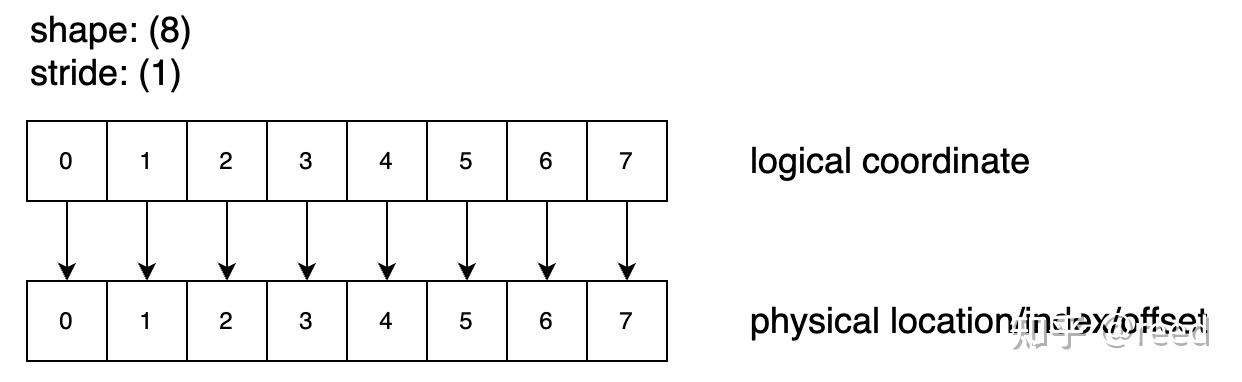
\includegraphics[width=0.9\textwidth]{figures/reed-01-layout/fig-01.jpg}
\end{figure}

Figure 1. shape = 8, stride = 1的逻辑空间和物理空间映射关系

Shape: (8), Stride: (2)表示该排列包含8个逻辑位置，每一个位置的坐标为自然序列0-7，如图2所示，其对应物理位置映射时的公式为 index\_physical = index\_logical * stride; 这时候我们发现逻辑空间和物理空间的大小是不一样的，在cute体系下，逻辑空间可以被称作domain，而代表存储的物理空间称作codomain，也就是size(tensor) = 8, cosize(tensor) = 15.

\begin{figure}[htbp]\centering
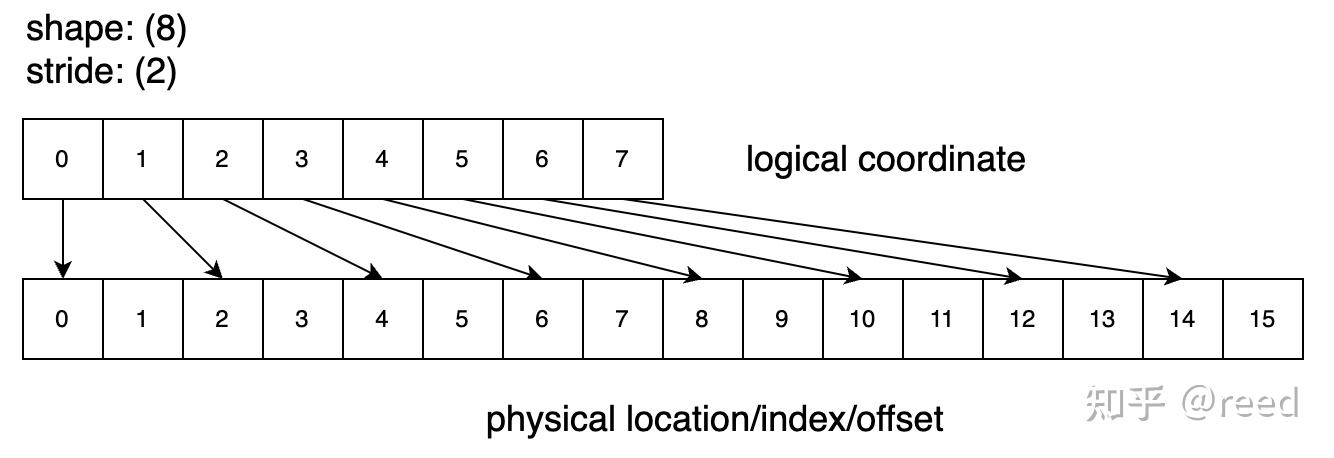
\includegraphics[width=0.9\textwidth]{figures/reed-01-layout/fig-02.jpg}
\end{figure}

Figure 2. shape = 8，stride = 2的逻辑空间和物理空间的映射关系

Shape: (8), Stride: (0)表示逻辑上我们需要的8个数据都来自于同一个存储位置0，如图3所示，所有的元素都指向同一个物理位置，通过图示也可以看到该layout的cosize为1。

\begin{figure}[htbp]\centering
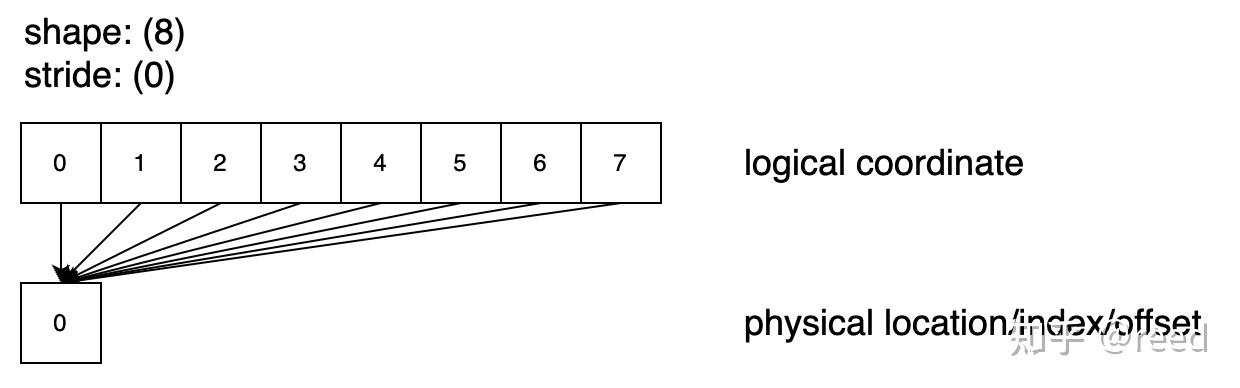
\includegraphics[width=0.9\textwidth]{figures/reed-01-layout/fig-03.jpg}
\end{figure}

Figure 3. shape = 8, stride =0的逻辑空间和物理空间的映射关系

Shape: (8), Stride: (-1) 通过Stride设置为-1可以实现对数据的前向访问，并且顺序是reverse的，这种case很少用到。

\begin{figure}[htbp]\centering
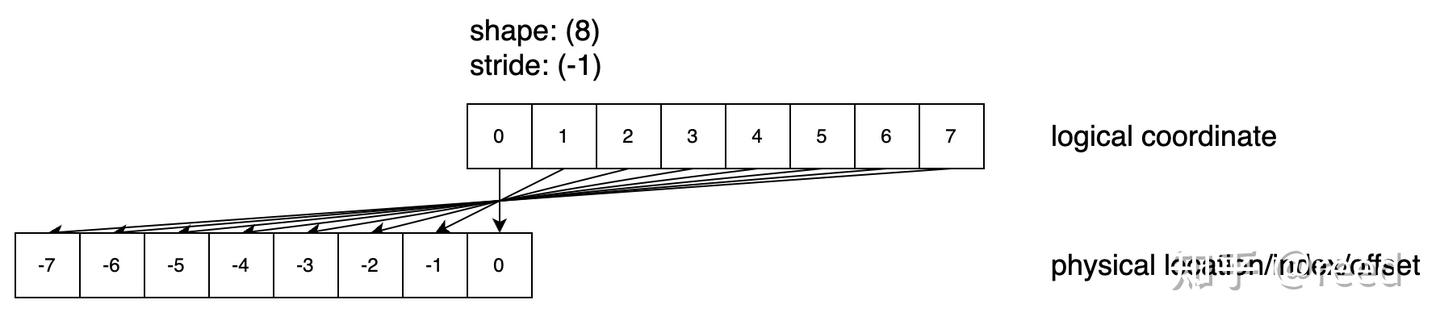
\includegraphics[width=0.9\textwidth]{figures/reed-01-layout/fig-04.jpg}
\end{figure}

Figure 4. shape = 8, stride = -1的逻辑空间和物理空间的映射关系

以上一维空间的示例，呈现了Tensor在其shape不变的情况下，通过stride的改变可以描述tensor中的各个元素在物理空间中的位置。我们在使用Tensor时候，关注的是其逻辑的大小，而通过stride则将这个逻辑空间和实际存储的物理空间进行了关联。并且在计算层面，我们可以看到其始终满足 index = coordinate * stride；

\section{二维矩阵的表示}

Shape: (3, 4), Stride: (1, 3)，和一维向量比较类似，此次的二维空间指的是Tensor的逻辑空间，其存储结构依然可以是一维的，二维空间的列优先描述可以表达为 shape(3, 4), stride(1, 3), 如图5，shape中的3，4分别表示矩阵的行数和列数，stride中的1，3分别表示元素沿着行增加1则物理存储相对的加1，而其中的3则表示如果元素沿着列增加1则其在存储空间的位置需要增加3。

\begin{figure}[htbp]\centering
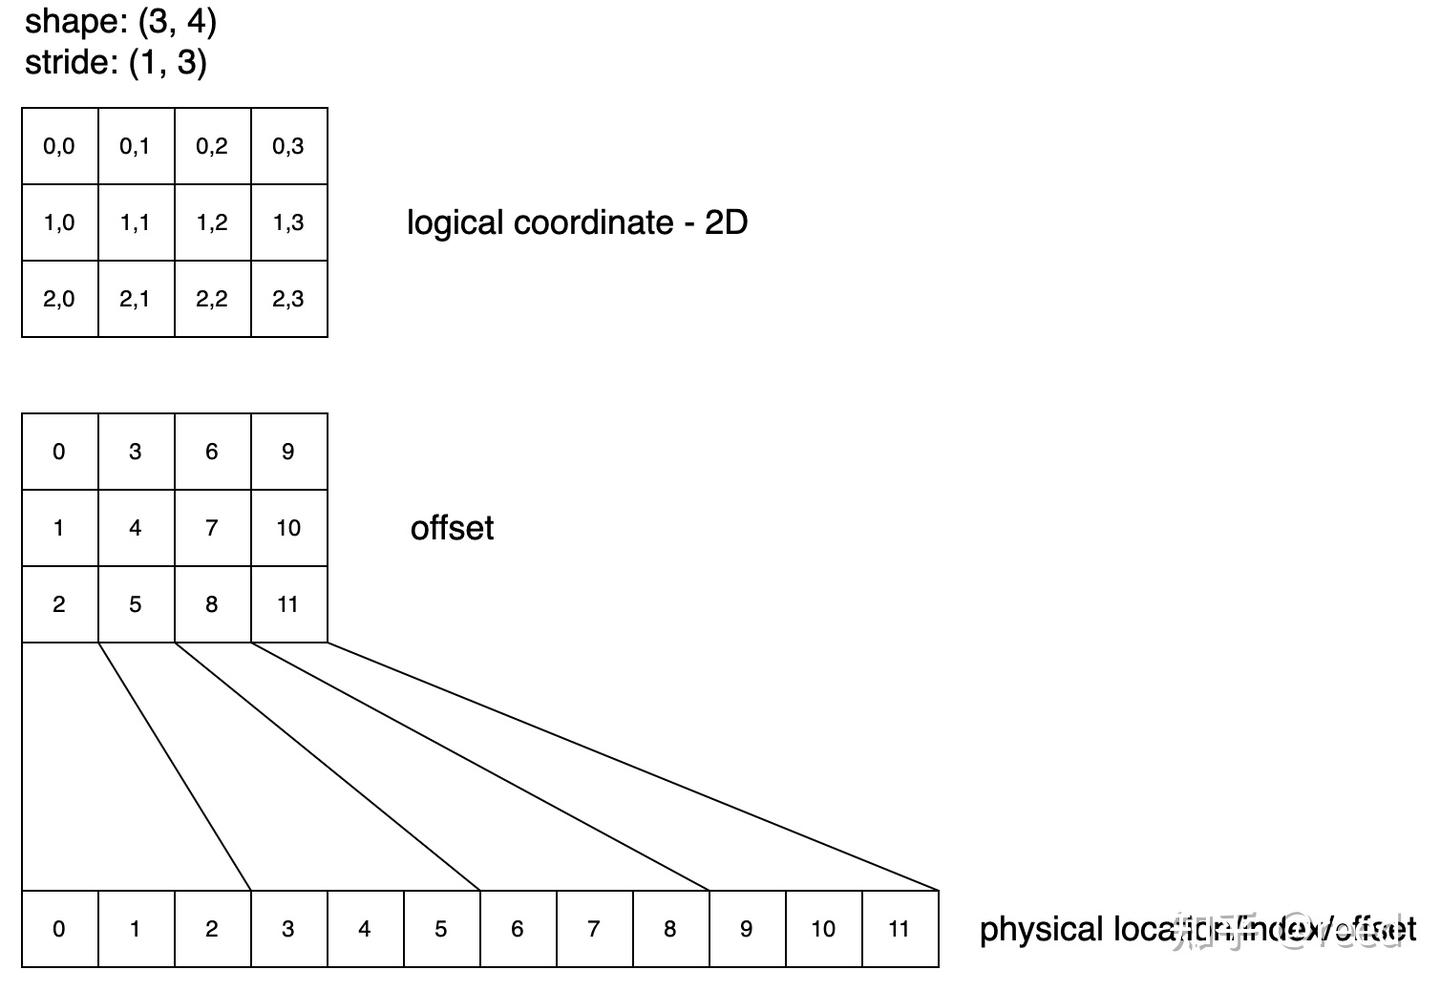
\includegraphics[width=0.9\textwidth]{figures/reed-01-layout/fig-05.jpg}
\end{figure}

Figure 5. shape = (3,4) stride = (1, 3)的逻辑空间和物理空间的映射关系

Shape: (3, 4), Stride: (4, 1)，和上面类似，Shape不变，而stride由(1，3)变为(4, 1)则存储结构变为行优先，即在物理存储数据的时候先存储每一行，行内元素存储的优先级高。

\begin{figure}[htbp]\centering
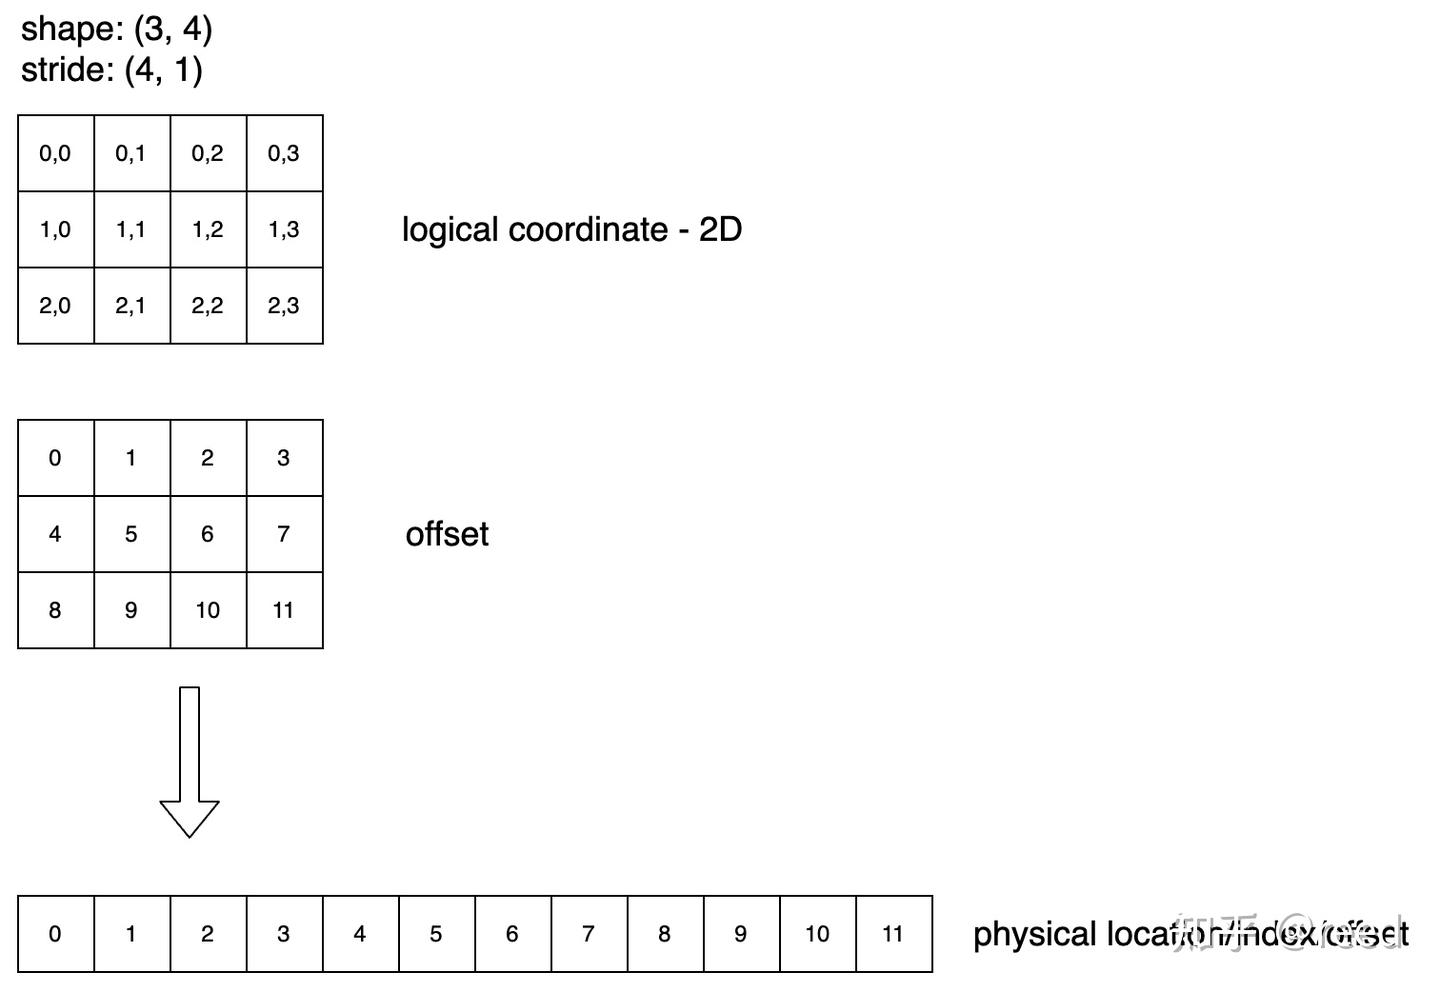
\includegraphics[width=0.9\textwidth]{figures/reed-01-layout/fig-06.jpg}
\end{figure}

Figure 6. shape = (3, 4) stride = (4, 1)的逻辑空间和物理空间的映射关系

二维矩阵的描述和一维类似，shape表示其逻辑形状，stride表示具体的某个元素和物理空间的映射时的间隔量。逻辑空间到物理空间的映射通过点积来完成。从二维空间我们可以很容易的扩展到高维空间，如深度学习常用的（N，H，W， C），其映射关系依然利用点积公式：

\begin{equation*}
index_{physical} = coordinate * stride = \sum_{i}{coordinate_{i} . stride_{i} }
\end{equation*}

\section{有层次的Layout（Heriarchy Layout）}

以上介绍的一维向量和二维矩阵描述描述被深度学习框架所广泛采用，在torch中我们可以访问tensor的shape属性和stride方法（注意方法调用需要使用带括号形式，即stride()）来获取对应的信息。我们不难发现，上面的shape和stride描述其限制了Tensor的每一个轴只能有一个stride值，也就是说，整个tensor在某一个维度上的连续性关系是不能变的，更形象地描述则为：Tensor不可以分块。我们将这样轴的连续性不可变更，体现为Tensor不可以分块的描述称为单调Tensor描述。而当我们处理复杂的Tensor计算问题时，尤其是如NVidia硬件引入的指令计算时，这种表示是不充分的。由此则引入了有层次的Tensor描述，即Heriarchy Layout。简单地理解，有层次的Tensor（或者Layout）就是以原有的单调Tensor所描述的小块作为基础单元，将其组成Tensor。这样原有的小块是Tensor，小块作为单元的外部组织也是Tensor，实现了Tensor套Tensor，这就是所谓的有层级的Tensor了。而其坐标到实际物理位置的映射关系则就是其Layout，Tensor有了层次，Layout也就有层次了。

\begin{figure}[htbp]\centering
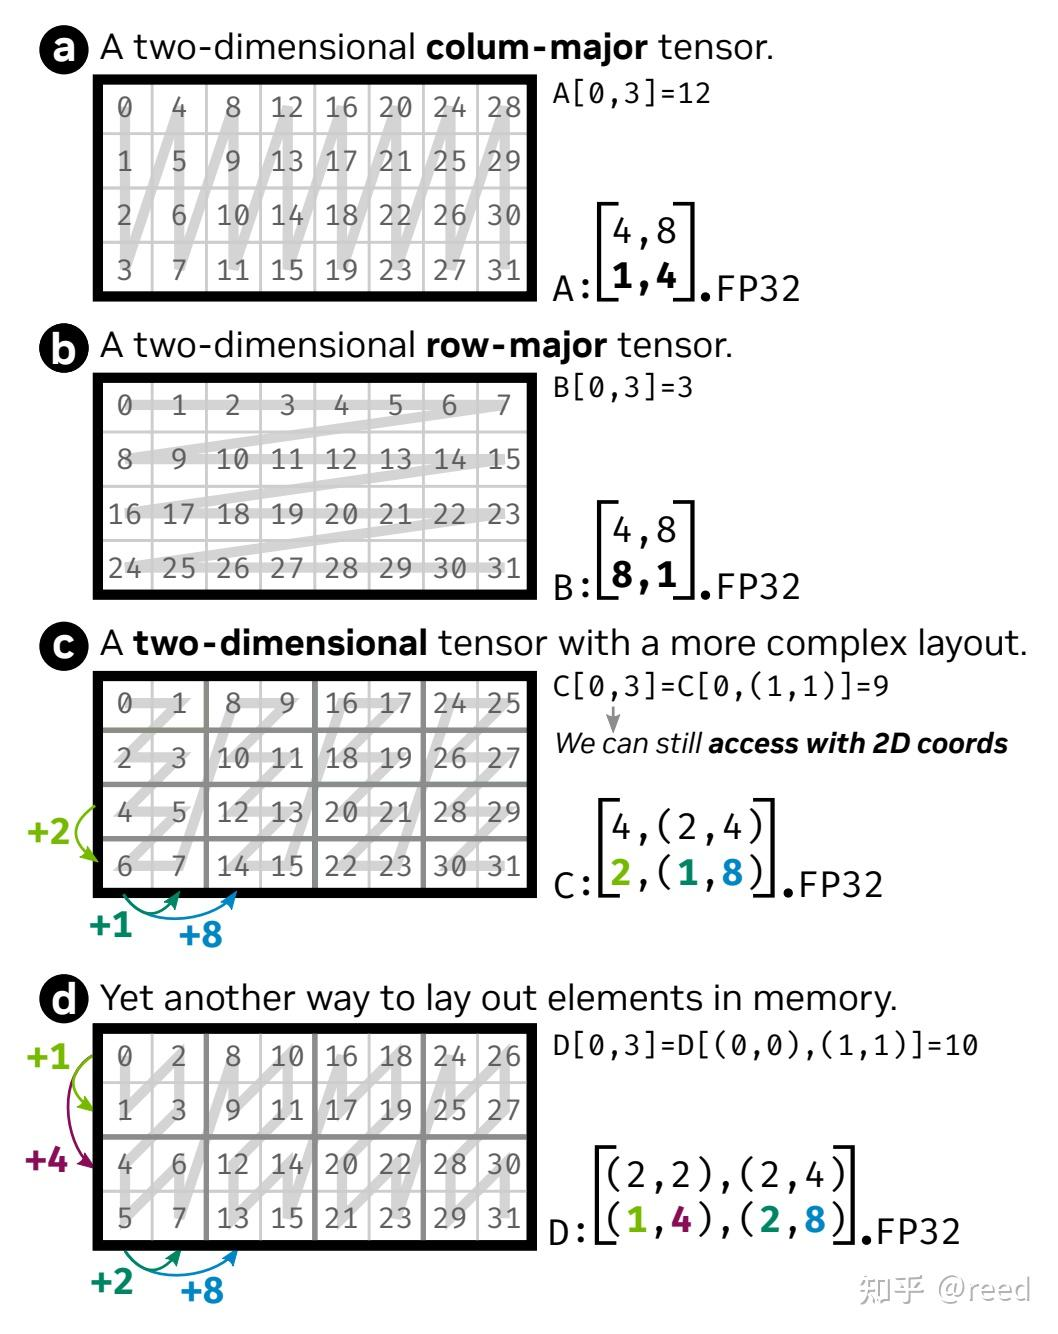
\includegraphics[width=0.9\textwidth]{figures/reed-01-layout/fig-07.jpg}
\end{figure}

Figure 7. 有层次的逻辑空间和其offset计算（引用自ASPLOS23 Graphene IR）

如图7-a/b，它们表示了传统的列优先和行优先的Layout，可以认为它们是一层的Tensor；而图7-c/d用之前的shape和stride描述没有办法表示如此复杂的情况（存在不单调的轴）。此时，我们可以将图7-c图看作两个层级的Tensor，如图8所示，其中内层Tensor为红框所标注的部分，外层Tensor为以红框作为元素的外层Tensor，内层Tensor的shape和stride描述可以表示为shape: (4, 2), stride: (2, 1)，外层Tensor的Layout可以表示为 shape: (1, 4), stride: (4, 1). 两层Tensor合并后，表示整体表示为 4行，8列，其中列方向为两个层次，即 8=2x4列，表示为(2, 4)列，其中2表示内层的Tensor维度为2，4表示列方向上外层Tensor有4个元素。即层级的shape 表示为 （4，(2, 4)）第一个4表示有4行，第二个4表示外层Tensor重复4列，2表示内层Tensor为2列。我们清楚了shape中的各个元素的含义后，stride的形式要与性状保持一致，即stride 要满足 (x, (y, z))的形式，根据x位置对应的含义，表示内层（红框内矩阵）矩阵的行方向的间隔，则有 x = 2；y为内层红框内列方向的间隔，有y = 1；z 则表示红框和红框之间横向的间隔，可以用第二个红框的左上角元素8和第一个红框对应的左上角元素0相减得到，即 z = 8 - 0 = 8, 这样我们得到有层次的Tensor的shape和stride描述：shape: (4, (2, 4)), stride: (2, (1, 8))。

\begin{figure}[htbp]\centering
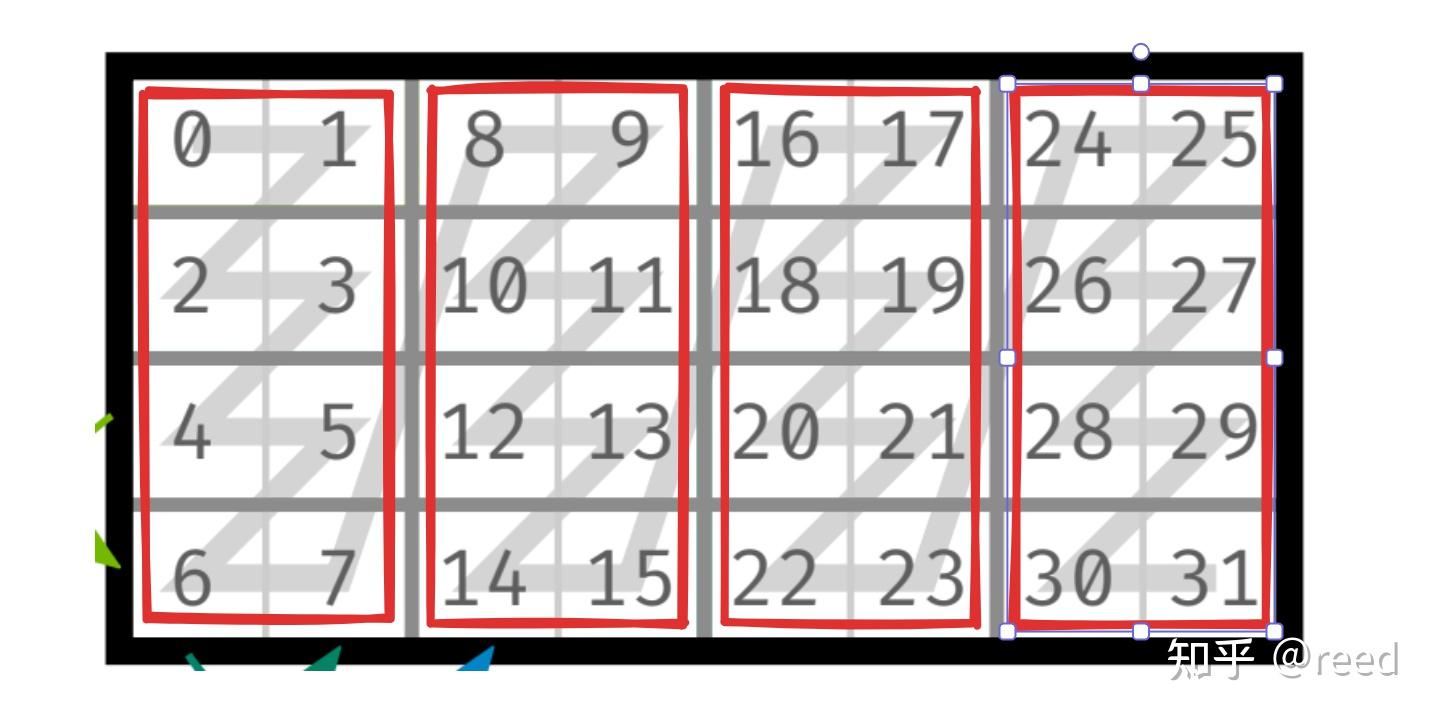
\includegraphics[width=0.9\textwidth]{figures/reed-01-layout/fig-08.jpg}
\end{figure}

Figure 8. 图7-c Tensor的层次分解

图7-d的层次分解和上面类似，其也是两层的结构（如图9）：内层的Tensor为红框所标注，shape: (2, 2), stride: (1, 2)；外层的Tensor为绿线所标注，shape: (2, 4), stride: (1, 2)；合并后的层次化表示 shape: ((2, 2), (2, 4))，其中的数字2，2，2，4分别表示内层Tensor行数，外层Tensor行数，内层Tensor列数，外层Tensor列数。同样的根据以上数据所表示的轴的信息，可以得到 stride: ((1, 4), (2, 8))。

\begin{figure}[htbp]\centering
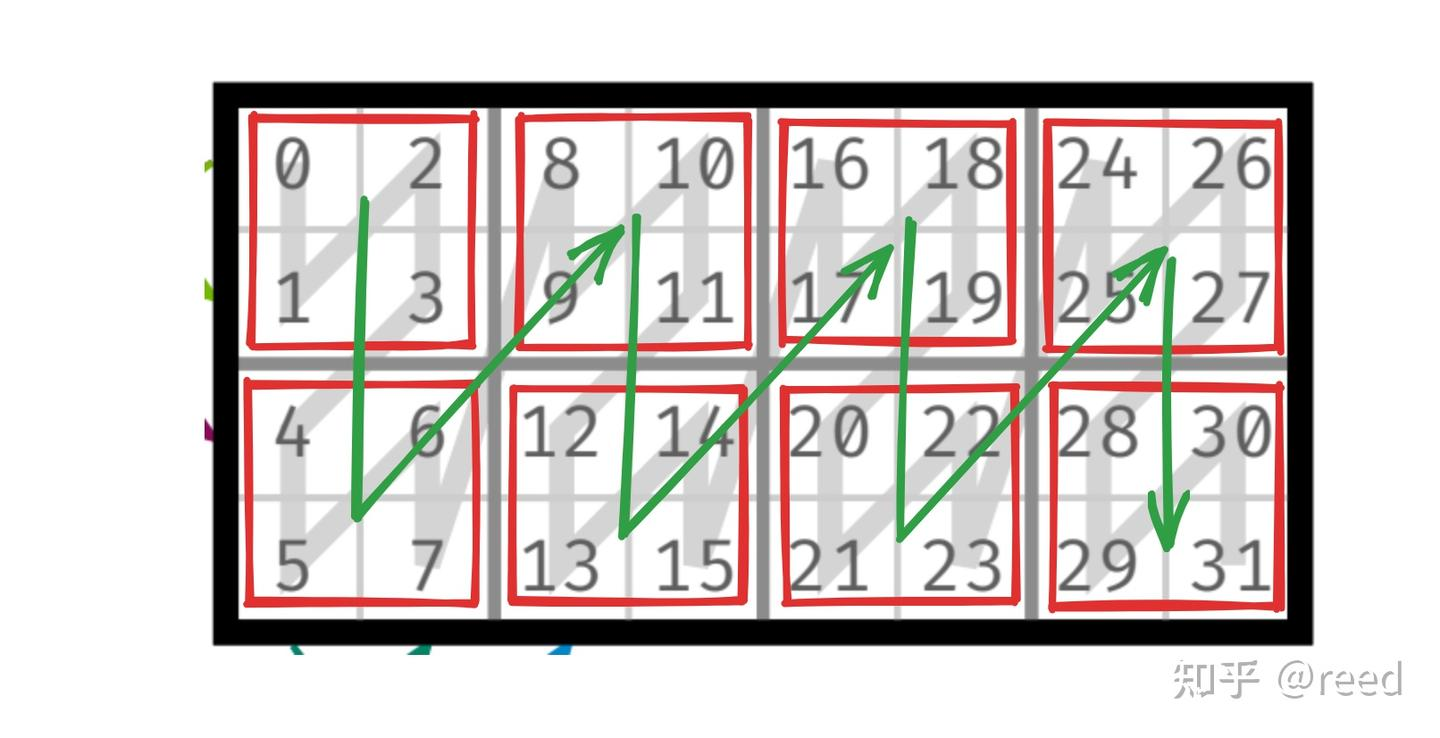
\includegraphics[width=0.9\textwidth]{figures/reed-01-layout/fig-09.jpg}
\end{figure}

Figure 9. 图7-d Tensor的层次分解

shape和stride给出了Tensor的逻辑空间描述和映射到物理空间时的间隔描述，当根据逻辑空间的位置获得物理空间位置时，依然和传统的Tensor计算规则一样，采用coordinate和stride点积即可，只不过坐标也采用heriarchy表达即可。

通过以上两个有层次Tensor的shape和stride的分解和组合，我们可以完成有层次的Tensor的组合，其突破了传统的Tensor轴只能有一个stride的限制，可以表达更丰富的Tensor（有层次的Tensor）。

以上介绍了有层级的Layout描述，具体的在cute实现时，其提供了make\_shape和make\_stride接口，并且make\_shape的参数可以接受make\_shape的结果，以此来完成有层次的shape和stride构建，为了提升效率，shape和stride可以区分为常量shape和变量shape。

\section{常量Shape（编译时Shape）}

常量Shape，即编译时Shape，可以通过在编译时完成坐标的映射或者推导，而减少运行时的计算量。对于需要编译时确定的量，需要用编译时常量来实现，如矩阵分块的大小其依赖了寄存器空间申请则必须使用这种类型shape，其书写形式为Int$<$K$>$\{\}，其中Int表示编译时常量，K表示具体的数值，{}表示以前面的类型来构造一个对象（常量对象），实例如下：

\begin{lstlisting}[language=C++]
auto shape = make_shape(Int<2>{}, Int<3>{});
auto shape1 = make_shape(shape, Int<3>{});
\end{lstlisting}

\section{变量Shape（运行时Shape）}

有些维度信息是运行时决定的，如vector长度等，而且不需要编译时决策，则采用运行时计算模式，值得注意的是示例代码中的2，3虽然是常数，但是在cute的约定里，该形式表示变量。

\begin{lstlisting}[language=C++]
auto shape = make_shape(2, 3);
auto shape = make_shape(m, n);
\end{lstlisting}

\section{总结}

Layout的本质是函数，其可以实现由一种坐标系统变换到一个表示偏移量的标量，超参为Tensor的逻辑shape和stride，即

\begin{equation*}
offset = Layout^{shape}_{stride}(coordinate)
\end{equation*}

\section{参考}

\begin{itemize}
  \item \url{https://dl.acm.org/doi/abs/10.1145/3582016.3582018}
  \item \url{https://github.com/NVIDIA/cutlass/tree/main/media/docs/cute}
\end{itemize}

\section{参考}

\begin{itemize}
  \item \url{https://dl.acm.org/doi/abs/10.1145/3582016.3582018}
\end{itemize}

\input{chapters/reed-02-layout-algebra-geometry.tex}
\input{chapters/reed-03-tensor.tex}
\chapter{cute 之 Copy抽象}

\begin{center}\small 作者：reed（知乎 @reed-84-49，专栏「CUDA高性能编程」）\quad 原文：\url{https://zhuanlan.zhihu.com/p/666232173}\quad 抓取：2026-09-20\end{center}

前面文章介绍了cute中的MMA抽象\footnote{\url{https://zhuanlan.zhihu.com/p/663092747}}，通过MMA我们可以利用Tensor Core完成寄存器上的\verb|D = AxB + C|计算。对于GPU编程而言，输入数据一般来被存储在全局内存之上。这就涉及到如何高效地将全局内存上的数据运到Tensor Core MMA计算所要求的寄存器上的问题。数据搬运的数学描述是 \verb|D = S|,其中D和S是前文中介绍的Tensor结构\footnote{\url{https://zhuanlan.zhihu.com/p/663093816}}，分别表示目标Tensor（Destination）和源Tensor（Source）。 它们一般存储在不同的存储层次上，它们有各自的Layout描述\footnote{\url{https://zhuanlan.zhihu.com/p/661182311}}。本文我们将围绕该问题，重点介绍cute在数据搬运的方面的数据结构的抽象。在文章结构上，本文首先介绍CUDA GPU中的存储层次和矩阵计算相关的ldmatrix指令，然后总体介绍cute中Copy相关的数据结构和函数的抽象以及各个结构之间的相互关系；然后我们依次对各个数据结构的核心函数和成员进行介绍，最后我们总结cute对Copy的抽象。

\section{CUDA的存储层次和数据加载路径}

\begin{figure}[htbp]\centering

\includegraphics[width=0.9\textwidth]{figures/reed-04-copy-abstract/fig-01.jpg}
\caption{Figure 1. GPU的存储层次和数据搬运路径}
\end{figure}

经典的GPU存储层次如图1所示，主要有：片外存储结构-全局内存（global memory）；片上SM（stream multi-processor）内的shared  memory 和 L1 data cache，以及寄存器堆（register file）；以及在全局内存和SM之间的L2 Cache。具体地，全局内存（图中标记为绿色global memory）容量最大，在数据中心级A100显卡中存储空间可以达到80GB，采用HBM2e技术实现，最高带宽可达2TB/s；再往内层为L2 Cache，在A100-80GB上为80MB，带宽可达20TB/s; 再向内层为片上(on-chip)存储shared memory 和L1 data cache，shared memory 和 L1 data cache 共享192KB的空间，可以配置shared memory 和L1的大小，最大可将shared memory配置为164KB。离计算单元Tensor Core和CUDA Core（图中分别标记为TC和CUDA）更近的存储结构为寄存器堆（图中标记为Register File），计算单元计算所需要的数据必须来自寄存器（Ampere及之前架构如此，Hopper架构的Tensor Core可以直接读取存储在shared memory数据进行计算），是GPU中最快的存储结构，一个线程最多使用255个32bit的寄存器。对于一个用GPU进行计算的问题，其原始数据来自于全局内存，可以经过三条路径到达核心计算单元上（Tensor Core或CUDA Core）。第一条路径，如图中路径1所示，从global内存经过L2到达shared memory（L1 bypass），然后从shared memory到达寄存器；第二条路径，如图中路径2所示，从global内存经过L2到达L1然后到达shared memory，再从shared memory到达寄存器；第三条路径从global内存经过L2到达L1，然后到达寄存器。其中路径1和2只在Ampere及其之后的架构才支持。Ampere之前的架构从全局内存到寄存器只支持路径3，从全局内存到共享内存只能先通过3将数据加载到寄存器，然后通过路径4存储到共享内存。这些存储结构我们可以编程控制的部分为全局内存共享内存和寄存器，L1 Cache和L2 Cache是缓存机构，我们可以控制其bypass与否，同时我们也可以通过PTX指令modifier控制L2 cache的数据预取行为。

\section{高效的ldmatrix指令}

在矩阵计算的优化中，非常重要的一个技术是通过数据分块实现数据复用，数据复用可以减少对低层级存储器的访问数据量，提升数据访问效率继而提升总体计算效率。在GPU的实现中，可编程的数据复用发生在共享内存部分，即用户通过编程手段将部分数据加载到共享内存然后复用共享内存中的数据，实现数据由共享内存到寄存器，然后实现更高效的计算。前面MMA章节我们介绍了Tensor Core的基础信息，如果我们认真研究Tensor Core的汇编指令我们不难发现，参与计算warp内的线程只持有矩阵的部分数据，这些数据保存在线程的私有寄存器中（SIMT架构中，可以认为寄存器为线程所私有），warp内的所有线程的寄存器共同组成完整的矩阵计算数据。这是NVidia在SIMT架构下实现warp level的Tensor Core计算的创新实践。如图2所示，在SIMT意义下每个线程持有两个数据（如float16，可以表达为一个寄存器），warp内的32个线程共同构成64个数据，形成8x8的warp level的小矩阵，供Tensor Core计算用。

\begin{figure}[htbp]\centering

\includegraphics[width=0.9\textwidth]{figures/reed-04-copy-abstract/fig-02.jpg}
\caption{Figure 2. SIMT寄存器协作构成warp level矩阵}
\end{figure}

通过各个线程提供的寄存器可以完成warp level的矩阵表示和存储，利用Tensor Core则可以完成高效的存储在寄存器上的矩阵计算。就数据从共享内存到寄存器的加载方面而言，可以通过SIMT意义下的LDS（load shared）来完成，但是由于数据是分布在不同的线程的寄存器上连续性方面不友好。为了更极致的性能NVidia从Turing架构开始提供了专门针对这种场景的加载指令ldmatrix。如图3，其展示了SIMT形式的模式加载矩阵数据和ldmatrix协作式加载矩阵数据的对比，ldmatrix协作式加载可以通过线程提供共享内存的地址（提供16Byte数据）完成数据的加载然后将数据分配到warp中各个线程的寄存器中，实现了跨越SIMT寄存器边界的写出，而如果是SIMT形式的加载，则只能使用更窄的数据位宽，这也就需要更多的指令完成等量数据的读写，同时ldmatrix由于是单线程提供16Byte的数据地址，warp内所有线程可以提供16Byte x 32 = 512Byte的数据到寄存器的加载，单指令实现16x16 float16矩阵的加载，减少指令数提高调度效率，同时其可以在写出时合并矩阵转置能力（可以参考tensorcore中ldmatrix指令的优势是什么？\footnote{\url{https://www.zhihu.com/question/600927104/answer/3029266372}}）。通过ldmatrix可以实现warp level共享内存到寄存器的数据搬运，自然地，cute对这种数据搬运提供了对应的抽象能力。

\begin{figure}[htbp]\centering

\includegraphics[width=0.9\textwidth]{figures/reed-04-copy-abstract/fig-03.jpg}
\caption{Figure 3. SIMT形式加载矩阵数据和ldmatrix协作式加载矩阵的对比}
\end{figure}

\section{cute Copy抽象及其相互关系}

和MMA类似，cute对数据搬运提供了对数据搬运的数据结构抽象，主要包括\verb|CopyOperation|、\verb|Copy_Traits|、\verb|Copy_Atom|、\verb|TiledCopy|、\verb|ThrCopy|和拷贝函数\verb|cute::copy|。这些结构和函数共同完成对GPU各个层级存储之上的数据进行搬运的抽象和实现，具体地，

\begin{itemize}
  \item CopyOperation提供了指令级的数据搬运的封装，NVidia在不同的硬件架构、不同的存储层次之间数据搬运提供了不同的指令，如前文提到的\verb|ldmatrix|和\verb|LDS|等，还有针对Ampere架构的\verb|cp.async|等，我们在使用时只需要根据我们的硬件支持的指令情况和需要搬运的内存层次来选择已经提供的Operation即可;
  \item Copy\_Traits和MMA\_Traits类似，提供了CopyOperation类型没有提供，但是其使用者Copy\_Atom却需要的起到桥梁作用的信息；
  \item Copy\_Atom提供了指令级别不可分割的数据搬运的拷贝能力；
  \item TiledCopy是对Copy\_Atom的能力的封装通过重复拷贝执行单元的个数（增加执行线程）或者做多次的拷贝实现对原子能力的重复；
  \item TildCopy提供的是逻辑上的拷贝的概念，在具体的kernel执行之时，为了复合CUDA的编程范式，需要写成线程级别的指令，ThrCopy可以实现将大块的数据根据TiledCopy所描述的划分规则，通过提供当前线程的线程号threadIdx.x对大块的Tensor进行划分，得到当前线程为了完成\verb|D = S| 拷贝所需要该线程做的任务；
  \item cute::copy在ThrCopy提供了当前线程的任务之后，便可以通过copy函数触发具体的数据搬运指令。
\end{itemize}

\begin{figure}[htbp]\centering

\includegraphics[width=0.9\textwidth]{figures/reed-04-copy-abstract/fig-04.jpg}
\caption{Figure 4. cute Copy核心结构和其相互关系}
\end{figure}

如图4所示，在硬件和拷贝方向之上提供了了指令抽象CopyOperation，再往上形成D = S的拷贝逻辑抽象，包含指令级别所能完成的拷贝原子能力Copy\_Atom和对Atom重复后得到的TiledCopy能力，再逻辑之上针对具体的线程划分出具体的线程级的任务，通过cute::copy函数触发相应的拷贝任务，所有线程共同完成Tensor到Tensor的拷贝。下面我们针对每一个抽象层次，具体的介绍各个数据结构和抽象的细节。

\section{CopyOperation}

Operation封装了特定硬件支持拷贝能力。它一般通过PTX汇编指令（或CUDA实现）来完成，实现指令集的拷贝能力抽象，其定义了源数据类型和目标数据类型以及个数，同时提供copy函数供框架层调用，示例如下，源寄存器为一个uint128\_t(128bit数据)，目标寄存器位一个uint32\_t的数据：

\begin{lstlisting}[language=C++]
struct SM75_U32x1_LDSM_N {
  using SRegisters = uint128_t[1];
  using DRegisters = uint32_t[1];

  void copy(uint128_t const& smem_src, uint32_t& dst) {
    asm volatile ("ldmatrix.sync. ...\n");
  }
};
\end{lstlisting}

\section{Copy\_Traits}

traits补充了CopyOperation的信息，如其提供了执行operation所需要的线程数，源数据和目标数据的Layout排布情况，其描述了线程和数据的存放关系，即通过线程号和寄存器号可以得到数据的逻辑位置，同时提供RefLayout供线程级的数据拆分时实现retile能力，具体的定义如下，

\begin{lstlisting}[language=C++]
struct Copy_Traits<SM75_U32x1_LDSM_N> {
  // Logical thread id to thread idx (warp)
  using ThrID = Layout<_32>;

  // Map from (src-thr,src-val) to bit
  using SrcLayout = Layout<Shape <Shape <  _8,_4>,_128>,
                           Stride<Stride<_128,_0>,  _1>>;
  // Map from (dst-thr,dst-val) to bit
  using DstLayout = Layout<Shape <_32,_32>,
                           Stride<_32, _1>>;

  // Reference map from (thr,val) to bit
  using RefLayout = DstLayout;
};
\end{lstlisting}

\section{Copy\_Atom}

Atom将Operation和Traits进行封装和抽象，定义了内部数据类型，供形成TiledCopy和后续的ThrCopy分解任务时提取信息，如其继承来自Traits的线程情况和数据Layout情况，提供call方法实现对底层指令的调用入口，

\begin{lstlisting}[language=C++]
struct Copy_Atom<Copy_Traits<Args...>, T>
  : Copy_Traits<Args...>
{
  using Traits = Copy_Traits<Args...>;

  // Bit and Thr layouts from the Copy_Traits
  using ThrID        = typename Traits::ThrID;
  using BitLayoutSrc = typename Traits::SrcLayout;
  using BitLayoutDst = typename Traits::DstLayout;
  using BitLayoutRef = typename Traits::RefLayout;

  using ValType = T;

  void call(Tensor<TS,SLayout> const& src, Tensor<TD,DLayout>& dst);
};
\end{lstlisting}

\section{TiledCopy}

tiled抽象通过对Atom能力进行重复得到更大的块的拷贝能力，对Atom的重复可以通过提供线程-存储的Layout来提供，也可以直接通过提供Atom能力和MMA中的tiled\_mma实现，如\verb|make_tiled_copy_A/B/C|，因为MMA已经提供了计算\verb|D = AxB + C|时所需要的数据划分能力，当然这些函数时针对寄存器表达能力的，具体的模版参数和形参如下。除了描述对Atom的重复方式外，TiledCopy提供的核心函数时\verb|get_slice|和\verb|get_thread_slice|,其可以实现将逻辑Tensor的拷贝能力根据线程的id得到每一个线程的Layout描述的拷贝任务，所以以上两个函数的返回对象为ThrCopy：

\begin{lstlisting}[language=C++]
template <class Copy_Atom,
          class LayoutCopy_TV,  // (tid,vid) -> coord   [Need not be 2D...]
          class ShapeTile_MN>   // coord space
struct TiledCopy : Copy_Atom {
  ThrCopy get_slice(ThrIdx const& thr_idx)；
  ThrCopy get_thread_slice(ThrIdx const& thr_idx));
};

CUTE_HOST_DEVICE
auto make_tiled_copy_A(Copy_Atom<Args...> const& copy_atom,
                  TiledMMA           const& tiled_mma)
\end{lstlisting}

\section{ThrCopy}

thread copy是线程级别的拷贝的抽象，其通过TiledCopy调用\verb|get_slice|方法而得到，其核心函数为\verb|partition_S/D|和\verb|retile_S/D|,其中S和D分别表示source和destination，partition表示对一个大的逻辑Tensor进行划分得到当前线程的拷贝所需要的源Tensor和目标Tensor， 而retile系列的函数表示其输入的数据已经是当前的线程的私有的数据了，但是其可能不满足拷贝所要求的形状，需要将其变换到拷贝所支持的形状，形式如下代码：

\begin{lstlisting}[language=C++]
template <class TiledCopy, class ThrIdx>
struct ThrCopy {
 auto partition_S(Tensor&& stensor);
 auto partition_D(Tensor&& dtensor);
 auto retile_S(Tensor&& stensor);
 auto retile_D(Tensor&& stensor);
};
\end{lstlisting}

\section{cute::copy}

copy函数是拷贝的实际执行函数，调用该函数会触发线程级别的拷贝的发生，完成线程指令的执行，实现src到dst到数据拷贝指令，实现逻辑上的\verb|D = S|。我们用块状逻辑对数据进行拷贝的时候可能遇到边界处理的情况，这时可以通过copy\_if实现对某些数据拷贝的mask，从额避免非法的数据访问，其函数原型如下，

\begin{lstlisting}[language=C++]
void copy(TiledCopy const& copy, Tensor const& src, Tensor& dst);
void copy_if(TiledCopy const& copy, PrdTensor const& pred, Tensor const& src, Tensor& dst);
\end{lstlisting}

cute::copy和其他组件的相互关系如表格所示。

\begin{center}
\begin{tabular}{ll}
\toprule
功能 & Copy \\
\midrule
指令+存储类型 & CopyOperation \\
逻辑类型和形状要求 & Copy\_Traits \\
原子能力 & Copy\_Atom \\
块状能力(多个原子能力) & TiledCopy \\
线程级能力 & ThrCopy \\
数据拆分API & ThrCopy::partition\_S/D(), ThrCopy::retile\_S/D() \\
触发功能执行 & cute::copy(tiled\_copy, thr\_s, thr\_d); \\
\bottomrule
\end{tabular}
\end{center}

\section{总结}

cute提供了Copy能力来完成实现\verb|D = S|Tensor的搬运，其通过对指令、适配层、原子能力、块状能力和线程级别的抽象分别形成了数据结构\verb|CopyOperation|、\verb|Copy_Traits|、\verb|Copy_Atom|、\verb|TiledCopy|、\verb|ThrCopy|和\verb|cute::copy|,在这些抽象的帮助下，我们可以实现逻辑Tensor由一个存储单元向另一个存储单元的拷贝，而不用过多的关注指令细节。 这种能力和MMA一道共同构成cute下矩阵乘法的基础。在Copy和MMA抽象的帮助下我们可以在逻辑层次构造数据的搬运\verb|D = S|和矩阵乘法\verb|D = A x B + C|。

至此我们已经讲解了cute中的Layout、Tensor、MMA、Copy抽象，我们已经可以完成一个GEMM（GEneral Matrix Multiplaction）问题了。通过Tensor和Layout抽象我们可以实现对计算矩阵的分块；基于Copy抽象，我们可以完成块状矩阵A、B数据从global内存到寄存器的加载；通过MMA抽象我们可以利用Tensor Core完成寄存器上小块矩阵的乘法运算；再次通过Copy抽象，我们可以将寄存器上的结果拷贝到global内存，完成完整的GEMM运算。下一篇文章我们将利用Layout、Tensor、MMA、Copy能力完成一个简单的矩阵乘法。

\section{参考}

\begin{itemize}
  \item \url{https://docs.nvidia.com/cuda/parallel-thread-execution/index.html#warp-level-matrix-instructions-for-mma}
  \item \url{https://github.com/NVIDIA/cutlass/blob/main/include/cute/algorithm/copy.hpp}
  \item tensorcore中ldmatrix指令的优势是什么？\footnote{\url{https://www.zhihu.com/question/600927104/answer/3029266372}}
\end{itemize}

\input{chapters/reed-05-mma-abstract.tex}
\chapter{cute 之 Swizzle}

\begin{center}\small 作者：reed（知乎 @reed-84-49，专栏「CUDA高性能编程」）\quad 原文：\url{https://zhuanlan.zhihu.com/p/671419093}\end{center}

前面的文章我们介绍了GEMM中的流水线技术\footnote{\url{https://zhuanlan.zhihu.com/p/665082713}}，流水线的核心是将拷贝\footnote{\url{https://zhuanlan.zhihu.com/p/666232173}}和计算\footnote{\url{https://zhuanlan.zhihu.com/p/663092747}}并行或者说是将数据加载隐藏在计算过程中。矩阵计算中的数据加载是从全局内存到共享内存然后到寄存器。共享内存作为中间的媒介可以减少矩阵计算时对全局内存的访问数据量，从而提升计算访存比。共享内存为了提升访问的并行性采用多bank结构，这也造成了编程时的困难，cute通过提供swizzle抽象简化了逻辑空间和多bank存储空间的映射的复杂度。本文首先介绍了shared memory的多bank存储结构，之后介绍了矩阵计算中的ldmatrix指令对逻辑空间和存储空间的要求，再次我们介绍了异或运算的特性和Swizzle抽象，最后我们简单介绍了Thread Block Swizzle和对本文进行了总结。

\section{局部性原理和Shared Memory}

局部性原理（Principle of Locality）是计算机科学的基石之一，它包括空间局部性和时间局部性。其中的空间局部性（也叫数据局部性）是指对数据的使用会限制在一个相对临近的存储空间中。Cache是针对空间局部性的很好的解决方案，但是Cache的数据更新和替换逻辑一般会实现在硬件中，表现为不可编程。在SIMT（single Instruction Multiple Thread）编程模式下，线程私有的寄存器提供了线程级别的存储能力，有时线程间需要交换一些数据来协同的完成特定任务，为了追求更好的数据局部性和实现线程间的数据共享，提供可编程的、线程间可共享的Cache就显得尤其重要。CUDA在硬件SM（Stream Multiprocessor）上提供了Shared Memory存储机构，同时软件上通过提供了相应的读写接口和同步源语言来实现其读写、同步和可见性，这样线程块内的线程便可以通过共享内存完成数据共享，同时对于线程块公共使用的数据便可以存储在其中达到线程块级别的可编程的数据局部性。

由于Shared Memory是为线程块服务的，所以其必须能支持线程块内的线程并行的对其进行访问（包含数据读取和写入），为了保障Shared Memory存储结构在多线程并发读写下的效率（更低的Latency和更高的Throughput），其硬件被实现为多bank的模式，每个bank都是可以独立寻址的存储空间，bank之间可以并行的读写数据，相互之间不会影响。在NVidia的架构中，shared memory包含32个bank，bank中可寻址的基本单元为4byte，如图1所示，每个bank为黑框所包含的单元，用户看到的地址空间为箭头所示的方向，即相邻的4byte占用不同的bank。如图2，当32个线程同时访问32个不同的bank时，各个bank是并行执行的，其效率是最高的，即32个线程并发的访问32个bank中不同颜色的单元，是可以并行的，值得注意的是其中的线程编号（如图2中的T0所示）和bank中的行位置并没有连续性要求。如图3，如果某两个线程T0、T2要同时访问相同bank-2的不同地址，则这两次访问会被排队执行，即先访问该bank的一个地址，然后再访问第二个地址，这样两次访问在发射任务维度上（产生访问请求指令）时间维度上是并行的，但是在真正bank读写数据在时间维度上是串行的。这就是所谓的bank conflict。由于一个bank上有两次冲突，这种情况称为二路冲突（two-way conflict）。

\begin{figure}[htbp]\centering

\includegraphics[width=0.9\textwidth]{figures/reed-06-swizzle/fig-01.jpg}
\caption{Figure 1. 共享内存bank结构和地址连续方向}
\end{figure}

\begin{figure}[htbp]\centering

\includegraphics[width=0.9\textwidth]{figures/reed-06-swizzle/fig-02.jpg}
\caption{Figure 2. 无bank conflict的共享内存访问模式}
\end{figure}

\begin{figure}[htbp]\centering

\includegraphics[width=0.9\textwidth]{figures/reed-06-swizzle/fig-03.jpg}
\caption{Figure 3. 两路冲突的共享内存访问模式}
\end{figure}

为了减少指令数，我们在进行kernel优化时会采用向量化的读写指令（也叫大字长读写），如以128bit的形式读写共享内存，此时线程需要访问的单位数据量为16byte，32个线程需要访问的数据量为16byte x 32 = 512byte。完整的512byte需要4个phase才能完成访问，第一phase，T0-T7无bank conflict的访问所有bank，第二phase，T8-T15无bank conflict的访问所有bank，第三phase，T16-T23无bank conflict的访问所有bank，第四phase，T24-T31无bank conflict的访问所有的bank。这种情况也可以看作是：shared memory基本单元为16byte，总bank数为8，冲突与否的分析不在是32线程，而变成4个phase中的不同线程。如果采用64bit的访问形式，则相应的基本单元可以看作是8byte，总bank数目为16，冲突与否的条件变成两个phase内的线程是否冲突。整体上shared memory空间可以看作二维存储空间，其中列方向表示bank情况，行方向表示自由定义的大小。值得注意但是冲突与否是通过内存访问事务级别来判定的，具体的可以参考NVidia开发者论坛的讨论\footnote{\url{https://forums.developer.nvidia.com/t/how-to-understand-the-bank-conflict-of-shared-mem/260900}}。

\section{共享内存读取（ldmatrix指令）}

\begin{figure}[htbp]\centering

\includegraphics[width=0.9\textwidth]{figures/reed-06-swizzle/fig-04.jpg}
\caption{Figure 4. ldmatrix输入和输出数据}
\end{figure}

在GEMM流水线中，利用Tensor Core可以完成特定规格的矩阵计算乘计算（如 $D_{16\times8} = A_{16\times16} B_{16\times8}   C_{16\times8}$ ），其中矩阵数据A、B、C、D是通过warp内的所有线程提供一部分寄存器共同表示的。如图4中右侧的register file所示，其表示32个线程T0-T31每一个线程提供一个寄存器V0（4byte），共同表示形状为8x8 half类型的矩阵块多个8x8的块可以构成更大的16x16，16x8的块。前序文章已经介绍过，这部分数据可以利用ldmatrix指令通过warp level实现。针对一个8x8-half的寄存器表示的作为输出的矩阵块，ldmatrix其输入要求为8个shared memory地址，每个地址指向一个16byte共享内存中的数据，其中T0-Addr0指向的16byte数据经过ldmatrix会被分派到T0-T3的V0寄存器中。T1-Addr1指向的数据会被分派到T4-T7的V0寄存器中。通过ldmatrix指令便可以实现矩阵数据从共享内存到寄存器到加载，前面的介绍我们知道共享内存是有bank结构的，并且按照16byte的形式进行读取，所以T0-T7读取该数据时会被作为一个独立的phase，这就要求所有的16byte表示的8个数据必须分布在不同的bank，才能确保读取共享内存数据时不产生bank conflict。图5展示了一种ldmatrix时无bank conflict的布局形式。

\begin{figure}[htbp]\centering

\includegraphics[width=0.9\textwidth]{figures/reed-06-swizzle/fig-05.jpg}
\caption{Figure 5. ldmatrix指令无bank conflict时的bank占用情况}
\end{figure}

从数学逻辑上看，8x8-half的寄存器数据表示连续的矩阵块，共享8x16byte的内存也有很好空间局部性的矩阵块，但是从共享内存的存储逻辑上看，为了避免读取时的bank冲突，其必须分配在不同的bank中。所以其横向位置在共享内存排列时不是简单的逻辑向下排列，而需要横向（bank方向）错开来避免bank conflict。

\section{Shared Memory写入}

在GEMM流水线中数据的起点是全局内存，如图6所示，矩阵乘法所需要的寄存器数据来自于共享内存，共享内存数据来自于全局内存，数学逻辑上寄存器表示的数学空间和全局内存的位置是对应的。但是共享内存由于有bank的存在，其块状数据在共享内存存储时不是简单行列排列。需要根据ldmatrix的要求来避免冲突，这样从全局内存读取数据后写入共享内存时，也需要按照逻辑要求进行存储空间的映射。同时在全局内存向共享内存加载时，为了提升全局内存的读取效率需要考虑合并访存和L2 Cache line的情况，一般会要求其线程沿着线性地址的空间顺序排列，如图T0-$>$Tn所示。也就是说我们在做全局内存到共享内存数据搬运时，思考模型是逻辑空间，而执行时需要考虑存储空间以避免bank conflict。

\begin{figure}[htbp]\centering

\includegraphics[width=0.9\textwidth]{figures/reed-06-swizzle/fig-06.jpg}
\caption{Figure 6. 数据加载的逻辑空间和物理空间}
\end{figure}

\section{异或运算的封闭性和双射性}

计算机异或指令（符号表示为\textasciicircum{}）接收两个输入，对于1bit数据，如果输入的bit相同则输出0，如果bit不同则输出1。对于多bit数据，则针对各个位置进行1bit异或操作。如5\textasciicircum{}3 = b0101 \textasciicircum{} b0011 = b0110 = 6。异或计算满足交换律，结合率。同时对于集合 $S = \{ x, x \in[0, 2^n-1] \}$ 中的任意两个元素，异或所形成的输出满足封闭性。如图7，我们可以发现该结果满足双射性（bijective），以上这些性质可以通过集合理论来进行严谨的证明。

\begin{figure}[htbp]\centering

\includegraphics[width=0.9\textwidth]{figures/reed-06-swizzle/fig-07.jpg}
\caption{Figure 7. 使用异或避免共享内存bank冲突}
\end{figure}

图7中左侧的逻辑矩阵可认为是icol为1的共享内存，其在共享内存对应一个bank，即矩阵的逻辑位置为 $(irow = [0, 7], icol = 1)$ ，我们可以通过对column进行异或得到新的column作为bank值，即 $(irow = [0, 7], ibank = irow \wedge icol)$ 。如图7中右侧黑框标注的部分，可以看到这些数据被分配到了不同的bank中，在读写时可以避免bank conflict。

\section{Swizzle抽象}

cute中通过swizzle抽象来实现共享内存bank conflict的冲突解决。通过前面的描述我们知道，在整个计算体系中，我们需要的是二维的逻辑空间来描述矩阵块，但是为了避免共享内存的冲突，我们在共享内存存储数据时需要的是物理空间。回顾之前的介绍我们知道描述逻辑空间我们可以使用Layout（本质是函数）\footnote{\url{https://zhuanlan.zhihu.com/p/661182311}}，而为了避免bank 冲突，cute中定义了swizzle抽象，swizzle的本质也是函数，swizzle作用在layout上，即函数作用在函数上，复合函数复合的定义。Layout的作用是给定坐标返回offset，而swizzle的作用则是给定offset返回bank conflict free的offset。即 $offset_{bank\_conflict\_free} = Swizzle(Layout(coord))$ 。为了达成这个目的，Swizzle定义了三个参数: B、M、S。它们共同表达描述一维坐标向二维空间映射的三个层次。当我们把一个一维度坐标转换成二维坐标时，我们首先将一维中连续的几个元素作为新空间中的基础元素，然后描述该二维空间有多少行和列。其中一维坐标中连续的 $2^M$ 个元素构成二维空间中最基本的元素， $2^S$ 表示新的二维空间中有多少列， $2^B$ 表示新的二维空间中有多少行。

\begin{figure}[htbp]\centering

\includegraphics[width=0.9\textwidth]{figures/reed-06-swizzle/fig-08.jpg}
\caption{Figure 8. Swizzle的计算逻辑}
\end{figure}

如图8所示，当B = 1, M= 1，S = 2时，M描述了一维坐标连续的两个元素构成一个二维空间的元素，S描述了形成二维空间后的元素的个数，B描述了形成二维空间的行数，如此我们便得到了图2-D(a)，其二维空间包含二行四列，基本单元包含两个元素。然后我们对二维空间中的列坐标和对应的行坐标进行异或得到新的列号(icol = irow \textasciicircum{} icol)，形成2-D(b)。如果一维坐标映射后超过出了 $2^B$ 的大小，则超出的部分的行号从0开始记，但是offset上要加上前面的所有的元素个数。

在实际操作时，如我们有一块half类型，shape:(8, 32), stride: (32, 1)的共享内存，我们定义Swizzle$<$3, 3, 3$>$作用到该shared memory Layout上，形成 A = Composition(Swizzle$<$3, 3, 3$>$\{\}, Layout$<$Shape$<$8, 32$>$, Stirde$<$32, 1$>$$>$\{\}); 则Layout中有效的offset为0 - 256。Swizzle中M为3，所以8个元素形成一个新的最小的元素，即8x2byte = 16byte；Swizzle中S为3，所以2D空间中一行包含8个元素，则有8x16byte = 128byte，128byte为shared memory无conflict访问所有bank的最大宽度；Swizzle中B为3，则2D空间irow更新的间隔为8。如此则实现了将一个逻辑的空间向2D的shared memory空间的映射，其中列的宽度为128byte占满所有的bank，行列异或后得到新的列号，避免了在bank方向（亦即icol方向）的冲突。

\section{Thread Block Swizzle}

除了避免共享内存冲突的swizzle外，cute（cutlass）中还有另一种swizzle，为thread block swizzle，在以C为中心的任务划分模式中，如果没有Thread Block Swizzle，则任务块会按照线性的行优先或者列优先的顺序分配给所有的执行单元（如图9中SM0-3，假设硬件只有4个SM），进行Thread Block Swizzle后，可以形成如图9右侧所示的任务划分关系，在某些场景下，其可以提升L2 Cache的命中率，数学上表现为在相同的元素能覆盖更大的面积，同时这部分面积(A、B)能够很好的被L2缓存住，具体的可以参考cutlass中的thread block swizzle实现。

\begin{figure}[htbp]\centering

\includegraphics[width=0.9\textwidth]{figures/reed-06-swizzle/fig-09.jpg}
\caption{Figure 9. Thread Block Swizzle}
\end{figure}

\section{总结}

本文介绍了shared memory的bank结构和特征，以及通过行列异或实现bank的交错的方法。继而介绍了cute中Swizzle的抽象，最后介绍了优化L2命中率的Thread Block Swizzle方法。至此矩阵乘法优化的理论性部分已经全部介绍完毕，接下来的文章我们会基于这些方法完成高效的矩阵乘法。

\section{参考}

\begin{itemize}
  \item \url{https://en.wikipedia.org/wiki/Locality_of_reference}
  \item \url{https://on-demand.gputechconf.com/gtc/2018/presentation/s81006-volta-architecture-and-performance-optimization.pdf}
  \item \url{https://patentimages.storage.googleapis.com/44/ed/9d/7b0c401348f57b/US8108625.pdf}
  \item \url{https://patentimages.storage.googleapis.com/e7/27/98/de3cbfc7ab3b8c/US7680988.pdf}
  \item \url{https://github.com/NVIDIA/cutlass/blob/main/include/cutlass/gemm/threadblock/threadblock_swizzle.h}
  \item How to understand the bank conflict of shared\_mem\footnote{\url{https://forums.developer.nvidia.com/t/how-to-understand-the-bank-conflict-of-shared-mem/260900}}
\end{itemize}

\chapter{cute 之 Hopper前言}

\begin{center}\small 作者：reed（知乎 @reed-84-49，专栏「CUDA高性能编程」）\quad 原文：\url{https://zhuanlan.zhihu.com/p/1948048832794427610}\end{center}

\section{背景与动机}

之前的“cute之[1][2][3][4][5][6][7][8][9]”系列文章我们重点介绍了cute中的核心概念和抽象，并且基于这些概念和抽象，按照自低向上的方式逐步构建起了利用cute实现GEMM计算的核心框架，这些内容主要是以Ampere架构为基础进行的介绍。2022年3月，NVidia在GTC大会上发布了Ampere的后继硬件架构-Hopper架构[10]，并于同年10月份发布了其针对AI计算市场的旗舰级产品H100。如今已是2025年11月，经过3年的时间，该架构下的芯片已然成为各大数据中心的算力输出的核心产品，其构筑了当今AI计算的最核心力量。相较于前序的Ampere架构，Hopper架构上增加了很多功能feature，其编程范式也发生了一系列变化，这些feature和新范式组合在一起共同组成了核心矩阵计算能力。刚好我也由于工作上的原因有机会接触到Hopper架构的产品，所以形成此系列文章，一方面作为我个人学习认知的总结和沉淀，另一方面也分享给各位奋斗、挣扎[11]在CUDA进阶之路上的同仁们，希望它能澄清Hopper上的编程范式和结构，希望这个系列能够帮助到你们。

\section{系列内容规划}

总体构思上大概分为五篇来介绍该内容：

\begin{itemize}
  \item cute之Hopper MBarrier
  \item cute之Hopper TMA
  \item cute之Hopper WGMMA
  \item cute之Hopper 硬件流水线
  \item cute之Hopper 高效GEMM实现
\end{itemize}

\input{chapters/reed-08-hopper-mbarrier.tex}
\chapter{cute 之 Hopper TMA}

\begin{center}\small 作者：reed（知乎 @reed-84-49，专栏「CUDA高性能编程」）\quad 原文：\url{https://zhuanlan.zhihu.com/p/1965678344352731952}\quad 抓取：2026-09-20\end{center}

% 含 % 编码的跳转 URL 需 \urldef 预定义（\url 的 verbatim 读取在 \footnote 参数内失效）
\urldef\reedIXurlA\url{https://link.zhihu.com/?target=https%3A//docs.nvidia.com/cuda/cuda-programming-guide/04-special-topics/async-copies.html%23using-the-tensor-memory-accelerator-tma}
\urldef\reedIXurlB\url{https://link.zhihu.com/?target=https%3A//docs.nvidia.com/cuda/parallel-thread-execution/%23data-movement-and-conversion-instructions-bulk-copy}
\urldef\reedIXurlC\url{https://link.zhihu.com/?target=https%3A//patents.google.com/patent/US20230289292A1/en}
\urldef\reedIXurlD\url{https://link.zhihu.com/?target=https%3A//resources.nvidia.com/en-us-hopper-architecture/nvidia-h100-tensor-c}

在Hopper架构之前所有的数据拷贝都是多个线程共同完成的，它包含每个线程完成大致相似的地址计算，每一个线程最多单次完成16字节的数据加载，通过多次循环完成更大规格的数据搬运，但是在Hopper及其之后的架构中，为了提高数据的加载效率，减少复杂且容易出错的加载流程，NVidia在Hopper架构中将数据据搬运任务抽象成独立的硬件单元TMA（Tensor Memory Accelator）。借助TMA的能力，Hopper上可以实现高效的数据搬运。本文首先介绍了传统的SIMT编程模型以及该模型下的数据搬运，然后重点介绍了Hopper上的TMA能力和编程模型的变更，详细介绍了它的TMA描述符、发起拷贝任务等特点，最后文章介绍了cute对TMA能力的封装和抽象。

\section{SIMT编程模型中的数据搬运}

CUDA从一开始就选定了SIMT编程模型，从编程逻辑角度由宏观到微观看，每一个程序（kernel）由一个线程网格（kernel）组成，每一个线程网格由一个或多个线程块（block，也称为thread block）组成，每一个线程块由一个或多个线程（thread）组成（如图1）。线程网格具有一定的局部性，在线程网格内的多线程之间可协同的完成计算和同步。

\begin{figure}[htbp]\centering

\includegraphics[width=0.9\textwidth]{figures/reed-09-hopper-tma/fig-01.jpg}
\caption{Figure 1. SIMT Programming Model}
\end{figure}

编程模型是软件模型，其本质是对硬件结构和能力的抽象。SIMT编程模型之所以这样抽象，是由NVidia硬件的设计模式决定的。如图2所示，NVidia GPU硬件架构整体分为四层，最内层的执行单元为带有Predication能力的SIMD核心，其可以在单个cycle内向量化的完成浮点运算，图中FP32核心可以在一个周期内完成32个32bit的符合IEEE标准的浮点乘法、加法、乘加运算，可以通过Predicate来决定该lane是否执行。和FP32功能单元类似，NVidia硬件还提供了整数计算单元（INT32）、64bit浮点计算单元（FP64）、矩阵计算单元（TensorCore）、数据加载单元（LSU）和特殊函数单元（SFU，可以完成正弦、余弦、倒数、开平方、E指数、对数等计算），这些不同计算类型的单元组合的在一起形成一个多功能计算能力，同时组合上Warp调度器（warp scheduler）和分派单元（dispatch unit）共同形成subcore，其可以实现warp级别调度和执行能力。4个subcore组合在一块形成更大的计算能力，同时附加上L1数据缓存（L1 data cache）和共享内存（shared memory）形成流处理器（Stream Multiprocessor，简称SM），在SM上会有Barrier硬件单元能够协同多个subcore的数据同步和执行进度，共享内存提供本地局部的数据复用。多个SM组合在一起同时附加上L2缓存（L2 Cache）和高带宽内存（High Bandwith Memory）形成GPU设备（device）。

\begin{figure}[htbp]\centering

\includegraphics[width=0.9\textwidth]{figures/reed-09-hopper-tma/fig-02.jpg}
\caption{Figure 2. NVidia GPU Hardware Architecture Abstraction}
\end{figure}

软件上的Grid是硬件Device的抽象，并且通过调度单元使得数量有限的SM可以支撑远超其规格的grid大小。软件上的block是硬件SM的抽象，block内包含多个warp，block内线程间可以通过共享内存共享数据，可以做线程同步，本质则是硬件在SM层级提供了可编程的cache机构shared memory，同时提供了执行同步的barrier能力。当一个block使用的资源不多的时候，一个SM可以承载多个并行的block来提高资源利用效率。软件上的warp是对硬件subcore的抽象，单个warp内可以进行并行的计算，可以完成多种类型指令的计算任务。而带Predicate的SIMD核心则是线程的抽象，通过Predicate来mask掉某些不需要执行的lane，从而实现SIMT语义。

当我们使用GPU完成一个特定问题的求解时，本质是将任务拆分为可并行的更小的子任务，这些任务最终被分配到一个并行执行的FP32或者INT32等核心上执行。具体到每一个线程，其根据其所在的block号和thread号（CUDA中的blockIdx和threadIdx）来映射一个问题域的很小的计算逻辑。针对数据计算和加载都是这样的。整体可以表示为 $T = P(\rm{threadIdx}, \rm{blockIdx})$ 。根据任务的划分使用FP32/INT32/LSU等来完成对数据的加载和计算。

以上便是SMIT模型下GPU到工作逻辑，针对于深度学习场景，其计算面对的输入输出通常是高维的Tensor，而在任务划分后所需要完成的数据拷贝也是高维空间中的一块数据，如常用的GEMM类计算，在Ampere架构上每一个线程会负责的任务有：

\begin{itemize}
  \item 将数据加载到共享内存（使用INT32）
  \item 读取共享内存数据读取到寄存器
  \item 使用TensorCore完成矩阵乘加计算
  \item 将结果写出到共享内存
  \item 读取共享内存数据到寄存器
  \item 将寄存器数据写出到全局内存
\end{itemize}

不难发现以上GEMM计算相关的内存操作中涉及大量的共享内存的操作，原因是使用共享内存可以提高数据复用，减少对全局内存的访问量，减少对低带宽通路的占用，继而提升计算效率。但是针对全局内存和共享内存之间的读取和写入而言，其会涉及到大量的地址计算和繁琐的处理，以读取全局内存写入共享内存为例，其需要使用INT32单元计算全局内存上作为输入的数据的地址，使用INT32单元计算计算共享内存输出的地址，同时由于共享内存的bank结构，需要引入避免bank冲突的逻辑，也会消耗整数和逻辑ALU指令，除了做bank冲突处理，矩阵计算一般是按照块进行的，对于边界不能整除的场景（tile quantization），经常需要对读取进行mask掉，对于输出的共享内存部分则需要填充上零，也会引入额外的指令消耗。值得注意的是，在SIMT编程模型下，这些操作需要所有的线程参与。并且处理这类问题很容易出错，有统计表明，CUDA开发者90\%的时间是在处理数据访问相关的问题，换句话说CUDA类程序员大部分时间是在处理illegal memory相关的问题。

\section{高效的异步Tensor内存拷贝加速单元}

针对SIMT意义下这种硬件计算浪费、编程错误率高、开发效率低的问题，NVidia在Hopper架构上给出了全局内存和共享内存之间数据拷贝的软硬件协同的高效的解决方案。硬件方面提供独立的张量内存加速单元（Tensor Memory Accelerator简称TMA），它将数据拷贝相关功能进行抽象并高度集成，形成独立的硬件单元，使其能够完成从一维到五维的全局内存和共享内存之间的大块Tensor语义的拷贝，拷贝的同时能够配置避免共享内存bank冲突的Swizzle模式，同时可以配置超过边界（Out Of Bound，OOB）时的填充模式，为了提高拷贝和计算可并行的效率，这些拷贝是异步执行的，即SM在发起拷贝任务后可以立即进行其他的任务，线程并不会因为拷贝而被阻塞。软件方面也打破了之前SIMT的编程范式，不再需要所有的线程参与地址的计算和数据读取，而是只需要一个线程即可以发起大块的Tensor的拷贝任务。

\begin{figure}[htbp]\centering

\includegraphics[width=0.9\textwidth]{figures/reed-09-hopper-tma/fig-03.jpg}
\caption{Figure 3. TMA Connection Illusttation}
\end{figure}

如图3所示，TMA在硬件结构上和SM一一对应，其被布置在SM内部，Dispatch单元可以向TMA单元发送数据拷贝指令，该指令发送后TMA则可以异步的进行数据拷贝，完成全局内存到SM内Shared Memory上的数据搬运。

\subsection{TMA描述符（TMA Descriptor）}

使用TMA完成全局内存到共享内存到数据搬运需要两个阶段，第一阶段为定义TMA描述符，第二阶段为实施Copy阶段（Copy Operation）。TMA描述符（TMA Descriptor）是一段内存结构其描述了完成拷贝所需要的必要信息，如图4所示，TMA描述符中包含全局内存的描述信息，输入Tensor的全局内存地址，Tensor的Shape和Stride表示；以及单次拷贝的拷贝块的大小表示（如图CopyBox），和共享内存上Tensor的swizzle信息和oob信息。通过描述符中的信息TMA则可以获得输入Tensor的完整精准的描述以及实施拷贝时的需要拷贝的大小和数据量，同时知晓在向共享内存写入时应该如何做Swizzle。在拷贝实施阶段，即SM发射了拷贝任务，则需要SM向TMA提供TMA描述符位置信息，TMA单元感觉该位置读取上诉信息，还需要提供要拷贝的块的起点位置（如图xy所示）；当以共享内存作为目标时，还需要提供共享内存的地址和作为拷贝完成机制的mbarrier的地址。

\begin{figure}[htbp]\centering

\includegraphics[width=0.9\textwidth]{figures/reed-09-hopper-tma/fig-04.jpg}
\caption{Figure 4. TMA operation mechanism}
\end{figure}

对于TMA描述符的构建，CUDA提供了特定的Driver API  \lstinline|cuTensorMapEncodeTiled|如下所示，其通过输入内存描述等信息，构建了TMA等描述符（tensorMap），在使用TMA完成拷贝时需要将该描述符传递给CUDA Kernel。

\begin{lstlisting}[language=C++]
CUresult cuTensorMapEncodeTiled (
      CUtensorMap* tensorMap,
      CUtensorMapDataType tensorDataType,
      cuuint32_t tensorRank,
      void* globalAddress,
      const cuuint64_t* globalDim,
      const cuuint64_t* globalStrides,
      const cuuint32_t* boxDim,
      const cuuint32_t* elementStrides,
      CUtensorMapInterleave interleave,
      CUtensorMapSwizzle swizzle,
      CUtensorMapL2promotion l2Promotion,
      CUtensorMapFloatOOBfill oobFill);
\end{lstlisting}

目前TMA Descriptor传递给Kernel有三种形式。第一种使用\lstinline|const __grid_constant__| 修饰符通过Kernel Parameter传值的方法传递给kernel，如下

\begin{lstlisting}[language=C++]
__global__ void tma_desc_demo1(const __grid_constant__ CUtensorMap map);
\end{lstlisting}

第二种使用CUDA运行时API\lstinline|cudaMemcpyToSymbol|  将描述符拷贝到\lstinline|__constant__|修饰的device变量上。

\begin{lstlisting}[language=C++]
// device
__constant__ CUtensorMap device_tma_desc;

// Host
CUtensorMap host_tma_desc;
cudaMemcpyToSymbol(device_tma_desc, &host_tma_desc, sizeof(host_tma_desc));
\end{lstlisting}

第三种则是将TMA Descriptor存储在全局内存上，CUDA Kernel内部直接向TMA提供该描述符地址即可

\begin{lstlisting}[language=C++]
__global__ void update_tma(CUtensorMap *desc) {
  // update TMA Descriptor fields
  // update global memory shape / stride
  // update copy box etc.
}
__global__ void tma_desc_demo3(CUtensorMap *desc) {
  // pass desc to TMA operation
}
\end{lstlisting}

以上三种形式适用于不同的场景，第一种适用于从host端可以确定全局内存Tensor的情形，如固定长度的linear层对应的gemm，第二种和第一种类似但是需要多出一个拷贝类的API调用；第三种为需要动态修改全局内存中Tensor的维度等信息时采用的模式，如大模型中MoE（Mixture of Experts）层中的GroupGEMM实现时，矩阵的m轴是动态变化的，这时一般采用第三种形式。不论是那种形式，其本质都是一个大小为128字节的描述信息，只是这个信息是相对固定的还是在运行时会动态更新和变化。就效率方面而言，前两种方法CUDA驱动层能够确保描述符是在更高效的缓存系统中，所以TMA获取描述符时效率更高一下，第三种形式需要TMA单元从HBM经由L2 Cache来获取该描述符，会有一定的overhead，此时可以通过软件编程的角度在恰当的位置对描述符进行预取，使用的PTX指令和对应的SASS如下

\begin{lstlisting}
// PTX
prefetch{.tensormap_space}.tensormap [a];

.tensormap_space =          { .const, .param };

// SASS
UTMACCTL.PF [UR4] ;  // Uniform TMA Cache ConTraL PreFetch
\end{lstlisting}

上面的SASS指令也揭示了TMA单元为了提升操作效率会有TMA Descriptor的Cache机构。TMA在进行拷贝相关的任务时会有限从本地的cache机构中查找描述符信息，如果命中，则直接发起相应的拷贝任务，如果不能命中则会从更低级的存储机构中读取。

\subsection{发起拷贝任务}

TMA描述符精准的描述了全局内存的情况以及具体拷贝时的基本块，在具体的需要拷贝时可以通过PTX提供的指令实现，以全局内存到共享内存为例，具体指令为

\begin{lstlisting}
cp.async.bulk.tensor.dim.dst.src{.load_mode}.completion_mechanism{.level::cache_hint}
                                   [dstMem], [tensorMap, tensorCoords], [mbar] {, cache-policy}

.dst =                  { .shared::cta }
.src =                  { .global }
.dim =                  { .1d, .2d, .3d, .4d, .5d }
.completion_mechanism = { .mbarrier::complete_tx::bytes }
.load_mode =            { .tile, .im2col }
.level::cache_hint =    { .L2::cache_hint }
\end{lstlisting}

其中cp来自copy的缩写，表示其为数据搬运指令，async表示该指令为异步指令，指令执行后并不代表copy完成，而只是代表copy任务被发起，bulk表示为大块内存拷贝区别于Ampere架构中的\lstinline|cp.async|指令（Ampere中的cp.async指令依然是SIMT范式的指令），tensor用以指示是面向tensor的copy，即由Tensor到Tensor到块拷贝，dim用以指示tensor的维度信息（亦即rank信息）只支持一维到五维，dst和src用以指定copy的目的和源内存类型，分别是thread block中共享内存和全局内存，load\_mode用以指示TMA的加载模式，除了本文重点介绍的tile模式，还有针对卷积运算（convolution）的im2col模式，tile模式即块到块的模式，输入输出等大小，completion\_mechanism表示完成机制，此处为mbarrier::complete\_tx::bytes，表示完成机制为mbarrier，当拷贝完成时TMA负责将拷贝的字节数写入到mbarrier中的transaction bytes字段中（参考cute之Hopper MBarrier），同时通知其完成，level::cache\_hint表示使用的L2的cache的驱逐策略，如evict\_norm、evict\_first、evict\_last，根据数据复用的时间、空间局部性，可以选择恰当的L2驱逐策略，以提升L2的利用效率。

以上介绍了TMA发起拷贝的modifier属性，具体操作数方面，有dstMem用于指定输出的地址，示例这里指共享内存的地址，tensorMap和tensorCoords用以指定TMA Descriptor到地址和拷贝块的坐标，这里会根据modifier中dim选择的不同而输出的参数数目不同，mbar用以指定完成时的通知机制mbarrier的地址，cache-policy为可选项，其用以指定L2的驱逐策略。

特别的针对一维的场景，可以不指定复杂的TMA Descriptor，而是指定全局内存的地址和size来完成大块数据的搬运，针对全局内存到共享内存拷贝，PTX提供的异步拷贝指令如下

\begin{lstlisting}
// global -> shared::cta
cp.async.bulk.dst.src.completion_mechanism{.level::cache_hint}
                      [dstMem], [srcMem], size, [mbar] {, cache-policy}

.dst =                  { .shared::cta }
.src =                  { .global }
.completion_mechanism = { .mbarrier::complete_tx::bytes }
.level::cache_hint =    { .L2::cache_hint }
\end{lstlisting}

在modifier方面整体和tensor版本类似，只是不在需要tensor和dim modifier，参数方面也只需要指定global memory的地址和size即可，可以避免相对复杂的TMA Descriptor构建。虽然一维的拷贝不需要TMA Descriptor但是其整体工作范式依然是TMA模式而非传统的SIMT模式，其只需要一条指令即可以完成大块数据的拷贝，而无需所有线程参与拷贝任务。

\subsection{完成机制}

从以上的指令介绍可以看到，针对全局内存到共享内存采用了mbarrier作为完成机制，而针对共享内存到全局内存方向的拷贝则采用bulk group机制，即commit/wait机制，其类似Ampere中的cp.async，能够将之前发起的异步拷贝整体提交，提交之后通过wait指令可以实现对这些提交的完成确认，不同源和目的内存的完成机制如下图（引用自NVidia PTX文档）。

\begin{figure}[htbp]\centering

\includegraphics[width=0.9\textwidth]{figures/reed-09-hopper-tma/fig-05.jpg}
\caption{Figure 5. TMA completion mechanism(From NVidia PTX  ISA-9.1, chapter-9.7.9.25.4.1)}
\end{figure}

\subsection{Swizzle机制}

TMA Descriptor创建时为了避免共享内存的读取和或写入的冲突可以指定Swizzle模式，常用的有以下四种

\lstinline|CU_TENSOR_MAP_SWIZZLE_NONE|，
\lstinline|CU_TENSOR_MAP_SWIZZLE_32B|，
\lstinline|CU_TENSOR_MAP_SWIZZLE_64B|，
\lstinline|CU_TENSOR_MAP_SWIZZLE_128B|

\begin{figure}[htbp]\centering

\includegraphics[width=0.9\textwidth]{figures/reed-09-hopper-tma/fig-06.jpg}
\caption{Figure 6. Swizzle Pattern for TMA}
\end{figure}

图6展示了shared memory的bank情况，此处最小的单元表示为16字节，可以认为shared memory有8个bank，不同的bank对应不同的颜色表示。对于不做Swizzle的情况，即SWIZZLE\_NONE, 横向128字节为不同的bank，纵向不做swizzle故而每行的bank颜色和第一行一致。针对SWIZZLE\_128B场景，即SWIZZLE的边界为128B，第二行的128B需要按照16B的为列号和行号进行异或得到swizzle后的bank号，即\lstinline|ibank = irow ^ icol|。SWIZZLE\_64B的模式时，可以认为是SWIZZLE\_128B的第一行分为前后两个部分，第二部分，即后64B折返到第二行形成两行，第三行和第四行则可以认为是SWIZZLE\_128B的第二行的前后一半排列成两行。SWIZZLE\_32B以此类推。整体计算逻辑如下

\begin{lstlisting}[language=C++]
int banks[sizeh][sizew];
for (int irow = 0; irow < sizeh; ++irow) {
  for (int icol = 0; icol < sizew; ++icol) {
    int ioffset = irow * sizew + icol;
    int irow1 = ioffset / 8; 
    int icol1 = ioffset % 8;
    banks[irow][icol] = irow1 ^ icol1; 
  }
}
\end{lstlisting}

\subsection{Async单元和可见性保障}

通过上面的介绍我们了解到TMA可以异步的读写共享内存，传统的LSU也可以读写共享内存（即通过对\lstinline|__shared__| 内存进行读取和写入），但是TMA和LSU不共享操作流水线，这就造成TMA和LSU对shared memory操作的可见性方面需要额外的机制才能保障。

\begin{figure}[htbp]\centering

\includegraphics[width=0.9\textwidth]{figures/reed-09-hopper-tma/fig-07.jpg}
\caption{Figure 7. LSU and TMA has its own pipeline}
\end{figure}

TMA读取global的数据数据写入到shared memory中，此时通过mbarrier的wait机制可以可以确保线程块看到TMA读取的结果，通过LSU读取共享内存可以得到正确的结果。如果是通过LSU向共享内存写入数据，但是通过TMA读取，如果不进行额外操作则TMA可能读到错误的结果。如下示例，通过LSU先向共享内存写入数据然后调用线程块同步函数\lstinline|__syncthreads|，同步之后调用单线程的TMA读取共享内存，在时序上看似先向共享内存写入的数据，然后发起了TMA读取共享内存，但是在TMA发起后真正读取数据的时候，LSU对共享内存的写入可以依然在流水线上，并没有真正完成，这也不能保证对TMA对可见，所以TMA有可能读到错误的数据，如果在syncthreads后是一个普通的共享内存的读，则其由于其走相同的流水线，能够确保读取到正确的数据。

\begin{lstlisting}[language=C++]
__shared__ float sdata[1024];

sdata[idx] = idx;
__syncthreads();

if(elected) {
  TMA::copy(sdata, ...);
}
\end{lstlisting}

针对以上场景，则需要显式的通过fence指令来确保内存事务的一致性，更新后的代码为

\begin{lstlisting}[language=C++]
sdata[idx] = idx;
asm volatile("fence.proxy.async.shared::cta;\n");
__syncthreads();

if(elected) {
  TMA::copy(sdata, ...);
}
\end{lstlisting}

其中fence指令行能够确保fence之前的内存事务被追踪，确保TMA能够看到该内存屏障事务，\lstinline|__syncthreads|能够确保线程在执行层的同步，而不是可见性的同步，这样TMA发起的拷贝任务会等待fence事务完成后才能进行，能够得到正确结果，一定程度上可以认为有了fence语句之后，TMA可以看到LSU的写入完成并且会等待写入完成后才能开始其对共享内存的读取，所以能够得到正确的结果。

\subsection{其他方面}

除了上面介绍的TMA的基本的概念和用法，TMA还能提供Cluster内的Multicast能力，即读取一份数据可以组播给cluster内的多个block；除了上面提到的tile的拷贝能力，TMA还提供了针对convolution计算模式的image2column能力，完成复杂的坐标变换和数据排列。同时在TMA读取共享内存写出全局内存的时候，还可以在写出时合并Reduce能力，这部分能力可以在具体的使用场景中参考相关文档来使能。

之前提到了TMA提供了对TMA Descriptor对预取能力，TMA还提供了对数据的全局内存要读取的数据进行预取的能力，使得程序员能够在计算过程中对需要用到的数据进行预取，以提升访存效率。

由于TMA是单线程发起范式，在一个block和warp内有一个线程即可以完成大块数据的拷贝，所以在指令设计方面它属于Uniform指令的范畴，自然地它的参数也为Uniform寄存器，能够减少对general寄存器的使用。同时为了辅助这种单线程发起拷贝模式，NVidia提供了\lstinline|elect.sync| PTX指令来更好的实现leader线程的选取。

由于是大块的内存访问，出于对效率的考虑，TMA访问的内存会有对齐的要求，具体的对齐要求如下（参看NV的CUDA编程手册）

\begin{figure}[htbp]\centering

\includegraphics[width=0.9\textwidth]{figures/reed-09-hopper-tma/fig-08.jpg}
\caption{Figure 8. Aligment Requirement for TMA（from NV CUDA Programming Guide）}
\end{figure}

\section{cute封装}

针对TMA能力，不管是TMA Descriptor的创建、device端对拷贝的发起还是TMA Descriptor的预取、预访问Tensor的预取，以及fence能力等，cute都做了很好的封装，我们后续在完成Hopper上高效GEMM实现时也将使用这些封装。核心封装在cute的/arch/copy\_sm90\_desc.hpp文件和cute/arch/copy\_sm90\_tma.hpp文件中，简单摘录如下，在cute/arch/copy\_sm90\_desc.hpp文件中有对TMA Descriptor的预取的封装

\begin{lstlisting}[language=C++]
void prefetch_tma_descriptor(TmaDescriptor const* desc_ptr);

enum class CacheHintSm90 : uint64_t {
  EVICT_NORMAL = 0x1000000000000000,
  EVICT_FIRST = 0x12F0000000000000,
  EVICT_LAST = 0x14F0000000000000,
};
\end{lstlisting}

在cute/arch/copy\_sm90\_tma.hpp有对发起copy能力的封装，包含LOAD、SOTRE、REDUCE、1D能力、IM2COL和MULTICAST能力：

\begin{lstlisting}
struct SM90_TMA_LOAD{_MULTICAST}[_1D/2D/3D/4D/5D]/PREFETCH
struct SM90_TMA_LOAD_IM2COL{_MULTICAST}[_3D/4D/5D]
struct SM90_TMA_STORE[_1D/2D/3D/4D/5D]
struct SM90_TMA_REDUCE_ADD[_1D/2D/3D/4D/5D]
struct SM90_BULK_COPY_G2S/S2G
\end{lstlisting}

\section{总结}

SIMT的编程范式中需要每一个线程参与数据的读写，其需要处理复杂的边界、针对共享内存需要处理由于共享内存bank结构带来而引入的swizzle优化，这回消耗大量的整数计算指令，同时开发效率也会因此而降低，针对这些问题，将上面的这些计算和处理需求封装成独立的硬件单元TMA，其能够高效的完成数据在共享内存和全局内存之间的拷贝，同时可以通过配置方式处理swizzle模式，oob模式，减少了地址的相关计算，提高了编程的效率。这是NVidia对SIMT编程范式的一次突破。如果要使用TMA能力，需要构造TMA Descriptor和发起拷贝两个部分，以全局内存向共享内存拷贝为例详细介绍了相关的指令，并且介绍和解读了开发中可能会经常遇到的可见性问题。cute对该能力有相对全面且完整的封装，利用好cute可以很好的利用其TMA的能力，完成数据的高效拷贝。后续我们将介绍Hopper上另一个重要功能单元WGMMA，最后我们将利用TMA完成高效的数据加载，利用WGMMA完成高效的矩阵运算、利用MBarrier完成高效的协同，借助这三者的力量完成Hopper架构上高效的矩阵计算。

\section{参考}

cute 之 Hopper MBarrier\footnote{\url{https://zhuanlan.zhihu.com/p/1962636004235153810}}

cute 之 GEMM流水线\footnote{\url{https://zhuanlan.zhihu.com/p/665082713}}

cute 之 Swizzle\footnote{\url{https://zhuanlan.zhihu.com/p/671419093}}

cute 之 Layout\footnote{\url{https://zhuanlan.zhihu.com/p/661182311}}

cute 之 Swizzle\footnote{\url{https://zhuanlan.zhihu.com/p/671419093}}

\url{https://docs.nvidia.com/cuda/cuda-programming-guide/04-special-topics/async-copies.html#using-the-tensor-memory-accelerator-tma}\footnote{\reedIXurlA}

\url{https://docs.nvidia.com/cuda/parallel-thread-execution/#data-movement-and-conversion-instructions-bulk-copy}\footnote{\reedIXurlB}

\url{https://patents.google.com/patent/US20230289292A1/en}\footnote{\reedIXurlC}

\url{https://resources.nvidia.com/en-us-hopper-architecture/nvidia-h100-tensor-c}\footnote{\reedIXurlD}

\chapter{cute 之 TMA Descriptor编码与隐藏的第21bit}

\begin{center}\small 作者：reed（知乎 @reed-84-49，专栏「CUDA高性能编程」）\quad 原文：\url{https://zhuanlan.zhihu.com/p/2037200219700449995}\end{center}

在之前的文章"cute 之 Hopper TMA"中，我们介绍了 TMA（Tensor Memory Access）的基本概念和使用方式。TMA 用一个 128 字节的 opaque descriptor 描述 tensor 布局，硬件自动完成地址计算、越界 fill、swizzle 等工作。其中"越界自动 fill"是 TMA 对程序员最友好的承诺——你不需要手写边界 clamp，只要 tile 坐标超出 globalDim，硬件就会把越界元素填成 zero 或 NaN。

我们在研究 cuTensorMapEncodeTiled的编码逻辑、并在不同驱动版本间做对比验证时，在 control word 的 bit[21] 位置发现了一个行为差异。在我们测试的 580 版本驱动中，该 bit 会根据 tensor 数据量是否达到 128KB 而被设置；而在我们测试的 530 版本驱动中，该 bit 始终为 0。进一步的实验表明，当 bit21=1 时，TMA 硬件会跳过 OOB 边界检查，直接对越界 tile 计算地址并发起内存请求——如果目标地址恰好落在未映射的虚拟地址区域，就会触发 illegal memory access。

本文分三个部分展开：首先完整呈现 TMA descriptor 的 128 字节二进制布局（这是理解 bit21 位置的前提）；然后通过精确控制 GPU 虚拟地址映射的实验，验证 bit21 对 OOB 行为的影响；最后讨论这个未文档化 bit 在 tensormap.replace动态修改场景下引发的实际问题及规避方法。

\section{TMA Descriptor 的完整二进制布局}

cuTensorMapEncodeTiled 构造的 CUtensorMap 是一个 128 字节、128 字节对齐的 opaque 结构体。NVIDIA 官方将其定义为 opaque type，没有公开内部编码方式。通过对大量参数组合下的输出做 byte-level 对比分析，结合 TMA 指令对 descriptor 各字段的访问行为，我们还原了完整的二进制布局。

\begin{figure}[htbp]\centering

\includegraphics[width=0.9\textwidth]{figures/reed-10-tma-descriptor-21bit/fig-01.png}
\caption{Figure 1. TMA Descriptor Offset and Fields}
\end{figure}

\section{整体结构}

\begin{lstlisting}
Offset   Size    Field
------   ----    -----------------------------------------
 0- 7    8B      globalAddress (64-bit device pointer)
 8-11    4B      Control Word (bitfield, 见下文详解)
12-27   16B      globalStrides[0..3] / 16 (各 32-bit, little-endian)
28-29    2B      stride upper bits (每个 stride 的高 4 位, packed as nibbles)
30-31    2B      reserved (=0)
32-51   20B      globalDim[0..4] - 1 (各 32-bit)
52-54    3B      elementStrides (每维 3 bits, packed)
55-59    5B      boxDim[0..4] - 1 (各 8-bit)
60-63    4B      reserved (=0)
64-67    4B      smem box total bytes
68-71    4B      reserved (=0)
72-75    4B      smem swizzle stride
76-127  52B      reserved (=0)
\end{lstlisting}

几个关键字段的说明：

globalAddress (bytes 0-7): tensor 在 device global memory 中的起始地址。TMA 硬件以此为基地址，加上 coord $\times$ stride 计算每个 tile 的实际访问地址。这是 descriptor 中唯一的指针字段。

globalStrides (bytes 12-29): 除最内层维度外的各维 stride，以字节为单位除以 16 后存储。采用 36-bit 编码（32-bit lower + 4-bit upper nibble），支持最大 64GB 的 stride 值。最内层维度的 stride 隐含为 elemSize，不编码在 descriptor 中。

globalDim (bytes 32-51): 各维度大小减 1 后存储为 32-bit 值。TMA 硬件用此做越界判断——当 tile 的起始坐标超出此值时认为越界。这也是 \lstinline|tensormap.replace| 最常修改的字段。

smem box total bytes (bytes 64-67): 一次 TMA tile load 搬运到 shared memory 的总字节数。计算方式为 \lstinline|product(boxDim[i] / elemStride[i])| $\times$ \lstinline|baseSize|，其中 \lstinline|baseSize| 在 interleave 模式下为 interleave 粒度（16B 或 32B），否则为 elemSize。

\section{Control Word 的 bitfield 布局}

Control word（bytes 8-11）浓缩了 descriptor 的模式配置信息。通过逐 bit 变化各 API 参数并观察输出变化，我们确认了以下布局：

\begin{figure}[htbp]\centering

\includegraphics[width=0.9\textwidth]{figures/reed-10-tma-descriptor-21bit/fig-02.jpg}
\caption{Figure 2. Control Word bitfield}
\end{figure}

\begin{lstlisting}
bit 位置        含义
----------      ----------------------------
bits[ 3: 0]    tensor type (0 = tiled)
bits[ 6: 4]    tensorRank - 1
bits[10: 7]    internal dtype code (4 bits, 与 API enum 值有重映射)
bits[12:11]    interleave (0=none, 1=16B, 2=32B)
bits[14:13]    swizzle (0=none, 1=32B, 2=64B, 3=128B)
bit [15]       oobFill (0=zero, 1=NaN)
bit [16]       reserved (=0)
bits[18:17]    l2Promotion (0=none, 1=64B, 2=128B, 3=256B)
bits[20:19]    reserved (=0)
bit [21]       OOB protection control <- 本文主角
bits[31:22]    reserved (=0)
\end{lstlisting}

需要强调的是，以上布局完全基于实验还原，不来自任何 NVIDIA 公开文档。NVIDIA 未公开 CUtensorMap 的内部结构。

\section{开源参考实现}

为了方便开发者理解和调试 TMA descriptor，我们提供了 \lstinline|cuTensorMapEncodeTiled_impl.h|一个纯软件的参考实现，具备两项核心能力：

正向编码：给定相同的 API 参数，生成与 driver 580 输出 byte-level 一致的 128 字节 descriptor（含 bit21 逻辑）。我们在多组测试向量上验证了与官方驱动的完全一致性。

解析打印：给定任意 CUtensorMap，将其内部字段完整解码并格式化打印——包括 globalAddress、各维度 dim/stride/box、control word 中的每个 bitfield。

这在调试 \lstinline|tensormap.replace|后的 descriptor 状态时尤其有用：你可以直接将修改前后的 descriptor dump 出来，逐字段比对，快速定位不一致。

\section{bit21 的设置规则}

在我们测试的两个驱动版本中，bit21 的行为如下：

Driver 530: bit21 始终为 0，无论输入参数如何变化。

Driver 580: bit21 根据以下条件设置：

\begin{lstlisting}
bit21 = (product(globalDim[0..rank-1]) * elemSize >= 131072)  // >= 128KB
\end{lstlisting}

\begin{table}[htbp]
\centering
\begin{tabular}{llll}
\toprule
dtype & dims & total bytes & bit21 (driver 580) \\
\midrule
UINT8(fp8) & [256, 511] & 130816 & 0 \\
UINT8(fp8) & [256, 512] & 131072 & 1 \\
FLOAT16 & [256, 256] & 131072 & 1 \\
FLOAT32 & [128, 128] & 65535 & 0 \\
FLOAT32 & [128, 256] & 131072 & 1 \\
FLOAT32 & [32, 32, 32] & 131072 & 1 \\
FLOAT32 & [32, 32, 31] & 126976 & 0 \\
\bottomrule
\end{tabular}
\end{table}

阈值精确卡在 $2^{17}$ = 131072 字节。我们没有确认这个行为具体从哪个驱动版本开始引入——仅确认在 580 中存在、在 530 中不存在。

\section{bit21 的硬件语义：实验验证}

知道了 bit21 的设置规则后，关键问题是：它控制什么硬件行为？

\section{实验设计}

为了隔离 bit21 的影响，我们需要构造一个实验，使得除 bit21 外所有条件完全相同，然后观察 TMA 对 OOB tile 的处理差异。

实验构造的核心挑战在于内存映射。cudaMalloc 的 suballocator 内部会映射远大于请求大小的虚拟地址区域（我们实测 cudaMalloc(2MB) 的有效映射达到 4MB 以上）。这意味着常规分配下 OOB 地址大概率仍在有效映射内——TMA 读到"垃圾数据"而不是 fault，无法区分"跳过检查直接读了"还是"检查后 fill 了"。

因此我们使用 cuMemCreate + cuMemMap 精确控制映射边界：在连续的虚拟地址空间中只映射中间 1 个 page（2MB），前后都是 unmapped 区域。将 tensor 数据（100 行 $\times$ 256 列 = 25KB）放在 mapped 区域的末尾，使得 OOB tile（coord\_y=128）的计算地址一定落入末尾的 unmapped 区域。

\begin{figure}[htbp]\centering

\includegraphics[width=0.9\textwidth]{figures/reed-10-tma-descriptor-21bit/fig-03.jpg}
\caption{Figure 3. Memory Layout and OOB Address}
\end{figure}

实验流程分两个 kernel 完成：

Kernel 1（update）: 将模板 descriptor 拷贝到 shared memory $\rightarrow$ \lstinline|tensormap.replace| 修改 address 和 dim[1]=100 $\rightarrow$ \lstinline|tensormap.cp_fenceproxy| 写回 global memory

Kernel 2（load）: \lstinline|fence.proxy.tensormap| acquire $\rightarrow$ TMA load at coord\_y=128（OOB: 128 $>$ dim[1]=100）

两组实验的唯一差异是创建模板时的 dims——[256, 512] vs [256, 511]——前者导致 bit21=1，后者 bit21=0。

\section{实验结果}

\begin{table}[htbp]
\centering
\begin{tabular}{lll}
\toprule
模板dims & bit21 & OOB TMA Load结果 \\
\midrule
{[}256, 512{]} = 128KB & 1 & illegal memory access \\
{[}256, 511{]} $<$ 128KB & 0 & zero fill, 无fault \\
\bottomrule
\end{tabular}
\end{table}

两个场景中 \lstinline|tensormap.replace| 后的实际状态完全相同——globalDim[1]=100，base address 相同，OOB 坐标相同，目标物理地址相同（均落入 unmapped 区域）。唯一的差异是 control word 中的 bit21。

\section{硬件行为模型}

\begin{figure}[htbp]\centering

\includegraphics[width=0.9\textwidth]{figures/reed-10-tma-descriptor-21bit/fig-04.jpg}
\caption{Figure 4. TMA OOB Path for 21th Bit in Control Word}
\end{figure}

基于实验结果，我们得出 bit21 的硬件行为模型：

bit21=0: TMA 前端在发起任何内存事务之前，先比较 tile 坐标与 globalDim。如果 coord $\geq$ globalDim，该 tile 被判定为 OOB，硬件在本地生成 fill value（zero 或 NaN，取决于 oobFill 配置），不产生任何内存请求。即使目标地址完全不可访问，也绝对安全。

bit21=1: TMA 跳过上述前端检查，直接计算 globalAddress + coord $\times$ stride 并向内存子系统发起请求。如果该地址有效（落在已映射的 VA 范围内），TMA 会读到该位置的数据——可能是正确数据，也可能是不相关的垃圾。如果该地址无效（未映射），则触发 page fault，表现为 illegal memory access。

bit21 本质上是一个性能优化开关：对于大 tensor，跳过逐 tile 的边界检查可以减少 TMA 前端延迟。猜测NVIDIA 的设计假设是——大 tensor 的实际内存分配通常有足够的对齐和 padding，正常使用中 OOB tile 的地址不会落在 page 边界之外。

\section{当性能优化遇到动态 Shape}

理解了 bit21 的语义后，它引发实际问题的条件也就清楚了。

NVIDIA 提供了 \lstinline|tensormap.replace| 指令，允许 kernel 在 device 上动态修改 descriptor 的 globalDim、globalAddress 等字段——这是处理 variable-length sequence（如 LLM 推理中的 group gemm、variable-length attention）的标准做法。问题在于：tensormap.replace 修改 dim 时不会联动更新 control word 中的 bit21。

这意味着以下使用序列会产生一个自相矛盾的 descriptor：

\begin{enumerate}
  \item 用较大的 max shape 创建模板 descriptor $\rightarrow$ 因为 total $\geq$ 128KB，bit21 被设为 1
  \item 运行时通过 \lstinline|tensormap.replace|将 dim 缩小为实际值 $\rightarrow$ bit21 仍为 1（replace 不更新 control word）
  \item TMA load 遇到 OOB tile $\rightarrow$ bit21=1 $\rightarrow$ 跳过检查 $\rightarrow$ 计算地址
\end{enumerate}

在大多数场景下这不会 fault——因为 cudaMalloc映射的 VA 范围远大于实际分配，OOB 地址通常仍然"可访问"（只是读到垃圾）。但在以下条件同时满足时会触发 illegal memory access：模板 tensor 总大小恰好 $\geq$ 128KB（bit21=1）；运行时某些 batch/group 的实际 dim 远小于模板；对应的 OOB 地址刚好越过了实际的 page 映射边界（memory pool allocator 的分配边界、cuMemCreate精确映射等场景）。

这不是误用 API。用户通过 NVIDIA 提供的标准 API 路径正确编程，得到的 descriptor 却进入了一个语义不一致的状态：globalDim 字段说"tensor 只有 100 行"，bit21 却告诉硬件"这个 tensor 很大，不需要 OOB 保护"。CuTe 中的 \lstinline|tma_descriptor_cp_fence_release| 和 \lstinline|tma_descriptor_fence_acquire|也不涉及 bit21 的同步更新。

bit21 的引入使得 OOB 检查变为有条件的，但 tensormap.replace 的实现未能跟进这一变化——它更新了参与 OOB 判定的 globalDim 字段，却没有联动更新控制 OOB 检查是否执行的 bit21。这是一个优化引入后接口语义未完整适配的问题。

\section{规避方法}

\section{方法一：创建模板时强制清零 bit21}

在调用 cuTensorMapEncodeTiled 后、将 descriptor 交给 kernel 使用之前，在 host 侧手动清除 bit21：

\begin{lstlisting}[language=C++]
// 创建 descriptor
cuTensorMapEncodeTiled(&tmap, ...);
// 强制清除 bit21，确保 OOB 保护始终开启
uint32_t control;
memcpy(&control, (uint8_t*)&tmap + 8, 4);
control &= ~(1u << 21);
memcpy((uint8_t*)&tmap + 8, &control, 4);
\end{lstlisting}

这种方法简单直接，代价是大 tensor 可能损失一点 TMA 前端性能（需要逐 tile 检查边界）。对于绝大多数应用场景，这个开销可以忽略。

\section{方法二：在 \texttt{tensormap.replace}[2] 修改 shape 时联动处理 bit21}

如果需要保留 bit21 的性能优化（大 tensor 跳过检查），可以在每次 replace dim 后根据新的实际 tensor 大小重新决策 bit21。由于 tensormap.replace 不支持直接修改 control word，需要在 shared memory 中手动 patch 对应字节后再通过 \lstinline|tensormap.cp_fenceproxy| 写回：

\begin{lstlisting}[language=C++]
// 在 smem 中完成 replace 后，根据新 dims 更新 bit21
uint64_t new_total = (uint64_t)new_dim0 * new_dim1 * elemSize;
uint32_t* ctrl_ptr = (uint32_t*)((uint8_t*)&smem_tmap + 8);
if (new_total >= 131072)
    *ctrl_ptr |= (1u << 21);
else
    *ctrl_ptr &= ~(1u << 21);
// 然后执行 cp_fenceproxy 写回 gmem
\end{lstlisting}

\section{结论}

TMA descriptor control word 的 bit[21] 是一个未文档化的硬件标志。在我们测试的 driver 580 中，当 product(globalDim) $\times$ elemSize $\geq$ 128KB 时被设置为 1；在我们测试的 driver 530 中始终为 0。

bit21=1 时，TMA 硬件跳过 tile 坐标的越界检查（OOB fill 机制被禁用），直接计算并访问目标地址。

\lstinline|tensormap.replace| 指令修改 globalDim 时不联动更新 bit21，可能导致 descriptor 进入"dim 小但 bit21=1"的不一致状态，在 OOB 地址恰好落入未映射区域时触发 illegal memory access。

规避方式为：创建 descriptor 后强制清零 bit21，或在 replace 修改 dim 后根据新 tensor 大小手动更新 bit21。

本文涉及的全部代码更新在\url{https://github.com/reed-lau/cute-gemm/tree/main/tma-desc}包括：

\lstinline|cuTensorMapEncodeTiled_impl.h|：参考实现（正向编码 + 字段解析打印，与 driver 580 输出 bit-level 一致）

\lstinline|test_bit21_oob.cu|：bit21 OOB 行为的最小复现

main.cc + tests.txt：52 组测试向量的全量回归验证

\section{参考}

\url{https://docs.nvidia.com/cuda/cuda-driver-api/group__CUDA__TENSOR__MEMORY.html}

\url{https://github.com/NVIDIA/cutlass/blob/main/include/cute/arch/copy_sm90_desc.hpp}

\url{https://patents.google.com/patent/US20230289292A1}

\chapter{cute 之 简单GEMM实现}

\begin{center}\small 作者：reed（知乎 @reed-84-49，专栏「CUDA高性能编程」）\quad 原文：\url{https://zhuanlan.zhihu.com/p/667521327}\quad 抓取：2026-09-20\end{center}

前面的文章我们对cute提供的核心数据结构和抽象进行了一系列的介绍，包括Layout、Tensor、MMA和Copy。本文我们将利用这些概念和抽象实现一个简单版本的矩阵乘法。在介绍具体实现之前，我们首先介绍BLAS约定和深度学习对矩阵乘法的需求和约定，然后介绍cuda上的矩阵库cuBLAS和矩阵乘法任务到硬件执行单元的划分策略，最后我们从Tensor构建、切块、划分，执行、拷贝等方面结合代码实现具体介绍了矩阵乘法的实现，同时我们对该版本的实现选取了实际场景中遇到的问题规模进行了实验并对比了该实现的效率。

\paragraph{BLAS约定和深度学习约定}

在科学计算和数值分析领域，经常需要解决矩阵特征值、线性方程（代数）等问题，形成了如EISPACK、LINPACK、LAPACK数学求解库。这些库解决的是偏上层的数学问题，它们共同依赖了更加底层的、更基础的数学库BLAS（Basic Linear Algebra Subprograms）。BLAS总共分为三个层次：第一层是向量操作，如 $\boldsymbol{y} = \alpha \boldsymbol{x} + \boldsymbol{y}$ 计算问题；第二层向量-矩阵操作，如 $\boldsymbol{y} = \alpha \boldsymbol{A} \boldsymbol{x} + \beta \boldsymbol{y}$ 计算问题；第三层矩阵-矩阵操作，如 $\boldsymbol{C} = \alpha \boldsymbol{A} \boldsymbol{B} + \beta \boldsymbol{C}$ 。

$\boldsymbol{C} = \alpha \boldsymbol{A} \boldsymbol{B} + \beta \boldsymbol{C}$ 就是我们常说的GEMM（GEneral Matrix Multiplication）问题，它也是BLAS第三层次要求解的问题。其中的广义来自于 $\alpha$ $\beta$可以是任意数值，$\boldsymbol{A}$和$\boldsymbol{B}$可以是转置的也可以是非转置的，数值精度方面可以是单精度浮点数、双精度浮点数等。BLAS早期实现的时候采用的是数值计算领域的Fortran语言，在Fortran语言中二维数组是列主序的（列优先），所以在BLAS的API中针对AB矩阵的转置情况描述而言，列优先称为Normal（简写为N），行优先则称为Transpose（简写为T），值得注意的是转置与否是针对A B矩阵而言的， $\boldsymbol{C}$ $\boldsymbol{D}$ 矩阵必须是列优先的。同时为了区分不同的数值精度，BLAS规定了不同的简写，如单精度浮点为s（缩写自single precision）, 双精度浮点为d （缩写自double precision），单精度复数为c （缩写自complex），双精度浮点复数记为z。所以在附加上数据类型（如单精度浮点）之后函数名字就由gemm变为了sgemm（single precision general matrix multiplation）。同时BLAS约定了矩阵的维度，表示为 $\boldsymbol{D_{m,n}} = \alpha \boldsymbol{A_{m, k}} \boldsymbol{B_{k, n}} + \beta \boldsymbol{C_{m,n}}$ ,

其中的m，n表示行列数目，k为reduce轴上的数据维度。

深度学习中也有矩阵乘法所表达的网络层（如Pytorch中Linear层、Tensorflow中的Dense层），但是神经网络中该层的公式可以表达为 $y = x \boldsymbol{A} + b$，其中x为input，维度一般为（N, Cin）y为output维度为（N, Cout），b为bias（一般是boardcast语义，此处我们忽略掉）。我们在忽略掉bias同时采用BLAS的矩阵形式描述，则其公式可以变更为 $\boldsymbol{D} = \boldsymbol{A}\boldsymbol{B}$ ，我们可以发现深度学习中需要的也是矩阵乘法的语义，和BLAS类似但是又不完全相同，不同点一深度学习中的公式没有BLAS公式中的 $\alpha$, 不同点二深度学习中公式没有BLAS中的加法右侧项，不同点三输出的D是行优先的而非BLAS中的列优先。除了公式层面的差异外，深度学习中的层为了计算效率会选用比传统的BLAS中的数据类型更低的精度如半精度和整数量化精度。

由于深度学习的输出要求的是行优先的，而BLAS中的约定中输出矩阵D是列优先的，因此当我们借助BLAS类函数完成深度学习的矩阵乘法时，需要对BLAS的公式进行转置变换，即

$\boldsymbol{D^{T}} = \alpha \boldsymbol{B^TA^T} + \beta \boldsymbol{C^{T}}$ ，同时设置 $\alpha$ 为1， $\beta$ 为0。由于转置矩阵AB的顺序也发生了变化。使用BLAS实现深度学习矩阵乘法的伪代码调用如下

\begin{lstlisting}[language=C++]
// blas_gemm(D, A, B, trans_a, trans_b, m, n, k, alpha, beta) API specifaction;
//  D = alpha op(A) op(B) + beta C;
// op can be 'N'ormal or 'T'ranspose
// output:
//    D(m, n) column major
// input: 
//    A(m, k) column major
//    B(k, n) column major
//    C(m, n) column major

// D(m, n) row major
// A(m, k) row major
// B(k, n) column major
void linear_layer(T *D, const T *A, const *B, int m, int n, int k) {
  T alpha = 1;
  T beta = 0;
  blas_gemm(D, B, A, 'T', 'N', n, m, k, alpha, beta);
}
\end{lstlisting}

\paragraph{NVidia cuBLAS类库}

NVidia使用GPU进行了BLAS加速实现，形成了cuBLAS加速库，cuBLAS除了实现BLAS中的API（Application Programming Interface）还扩展实现了多Batch支持、多GPU支持和针对深度学习加速的混合精度、低精度实现。对于我们深度学习中常用半精度（half precision）的gemm类似于之前的sgemm，在cuBLAS中提供了hgemm（half precision general matrix multiplation）。本质而言cuBLAS是一个大的kernel仓库，其中存储了NVidia针对不同数据类型，计算精度、矩阵维度、地址对齐等维度综合考虑的高度优化的kernel。当用户调用其进行矩阵运算时，cuBLAS会使用特定的方法从这些kernel中选择出一个针对该问题规模和约束的性能较好的实现版本。除了cuBLAS外，NVidia同时针对不同功能需求和性能追求提供了cuBLASLt库等，如图1所示，其对比了NVidia提供的BLAS类库的API复杂度和融合后处理能力。

\begin{figure}[htbp]\centering

\includegraphics[width=0.9\textwidth]{figures/reed-11-simple-gemm/fig-01.jpg}
\caption{Figure 1. NVidia提供的BLAS类的库对比（引用自参考5）}
\end{figure}

cuBLASLt库是cuBLAS库的基础上提供针对人工智能和机器学习更灵活的应用，它允许用户指定更复杂的输入输出类型、计算类型（解决混合精度的多类型指定问题）等，同时它还提供了启发式算法，允许用户选择底层实现的性能更好的kernel。后续的文章中我们的实验会利用cuBLASLt的这种选择kernel能力，选择候选kernel中最好的那一个作为我们的baseline。本文中实验我们使用cuBLAS选定的kenrel作为baseline。

\paragraph{Tensor表示}

\begin{figure}[htbp]\centering

\includegraphics[width=0.9\textwidth]{figures/reed-11-simple-gemm/fig-02.jpg}
\caption{Figure 2. 矩阵乘法问题的Tensor表示及其属性}
\end{figure}

如图2所示，本文我们研究深度学习中常用的C = AB的矩阵乘法问题，其中矩阵A、B存储在GPU的全局内存中，输出C矩阵将会被存储在全局内存中；维度方面A为m行k列，B为k行n列，输出C为m行n列；数据存储Layout方面，A为行优先，B为列优先，C为行优先。数据类型方面A、B、C都位16bit的半精度浮点数，在cuda中表示为half类型（cute封装为\lstinline|cute::half_t|类型）。我们将矩阵ABC的信息形成如下表格，同时将row/column major表示为stride形式，填充上指针变量名称

\begin{table}[htbp]
\centering
\begin{tabular}{llllll}
\toprule
矩阵 & 指针变量 & 存储位置 & shape & stride & 数据类型 \\
\midrule
A & Aptr & global memory & (m, k) & (k, 1) & half \\
B & Bptr & global memory & (k, n) & (1, k) & half \\
C & Cptr & global memory & (m, n) & (n, 1) & half \\
\bottomrule
\end{tabular}
\end{table}

我们将ABC表示为Tensor形式，则可以写出如下kernel代码

\begin{lstlisting}[language=C++]
template <typename T>
__global__ void gemm_simple(T *Cptr, const T *Aptr, const T *Bptr, int m, int n, int k) {
  Tensor A = make_tensor(make_gmem_ptr(Aptr), make_shape(m, k), make_stride(k, Int<1>{}));
  Tensor B = make_tensor(make_gmem_ptr(Bptr), make_shape(n, k), make_stride(k, Int<1>{}));
  Tensor C = make_tensor(make_gmem_ptr(Cptr), make_shape(m, n), make_stride(n, Int<1>{})); 
}
\end{lstlisting}

其中\lstinline|make_gmem_ptr()| 函数用于标识tensor指针的存储层次，方便后续使用时能从指针中取出该指针的存储层次。同时，我们修改了Tensor B的矩阵表示形式把它的形状表示(n, k)，对应的stride 为(k, 1); 这样后续的循环的时候我们就可以写成reduce的形式。为了编译时决策和优化，我们把stride中的连续维度1表示为编译时常量的形式，即\lstinline|Int<1>{}|，这样后续对矩阵进行操作的时候如果需要用到stride的计算则可以利用编译时的决策和优化减少不必要的运行时运算。

\paragraph{以C矩阵为中心的任务划分策略}

GPU中有多个SM（Stream Multiprocessor）我们编程时以grid、block的软件层级进行编程来利用这些SM，在矩阵计算中，我们以输出矩阵C作为划分thead block的单元进行任务拆分，也就是说一个thread block完成C矩阵中的一个小块（TileC）的计算任务，如图3所示，我们定义矩阵TileC的大小为kTileM、kTileN，分别表示小块矩阵包含元素的行数目和列数目，根据块状矩阵乘法的公式完成TileC的计算需要A矩阵中的绿色高亮部分和B矩阵的黄色高亮部分，它们的形状分别为(kTileM, k)和(kTileN, k)。我们对AB矩阵的k轴按照kTileK的大小进行分块，则可以将TileC矩阵表达为AB矩阵块的点积运算

\begin{equation*}
TileC = \sum_{itile = 0}^{num\_tile}{TileA_{itile} TileB_{itile}}
\end{equation*}

\begin{figure}[htbp]\centering

\includegraphics[width=0.9\textwidth]{figures/reed-11-simple-gemm/fig-03.jpg}
\caption{Figure 3. sliced-k模式的C矩阵为中心的任务划分方法}
\end{figure}

如此，我们在k轴上移动kTileK得到AB上的小块 $TileA_{itile}$ 和 $TileB_{itile}$ 将他们相乘的积累加到TileC上，便可以得到TileC的计算结果。这种沿着k轴移动的策略称sliced-k方法。这样我们使用一个block（坐标如图blockIdx.x, blockIdx.y）便可以完成C矩阵中一个小块的完整的计算。通过block维度的扩展，如图所示的矩阵C中M轴方向的blockIdx.y和N轴方向的blockIdx.x的扩展，便可以完成整个C矩阵的计算。由此我们可以计算出完成整个C矩阵所需要的gird维度：\lstinline|grid.x = N / kTileN, grid.y = M / kTileM| (此处暂时不考虑不可整除的情形)。根据上面的计算过程我们可以继续完善代码，

\begin{lstlisting}[language=C++]
template <typename T, int kTileM, int kTileN, int kTileK>
__global__ void gemm_simple(T *Cptr, const T *Aptr, const T *Bptr, int m, int n, int k) {
  Tensor A = make_tensor(make_gmem_ptr(Aptr), make_shape(m, k), make_stride(k, Int<1>{}));
  Tensor B = make_tensor(make_gmem_ptr(Bptr), make_shape(n, k), make_stride(k, Int<1>{}));
  Tensor C = make_tensor(make_gmem_ptr(Cptr), make_shape(m, n), make_stride(n, Int<1>{}));

  int ix = blockIdx.x;
  int iy = blockIdx.y;

  Tensor gA = local_tile(A, make_tile(Int<kTileM>{}, Int<kTileK>{}), make_coord(iy, _));
  Tensor gB = local_tile(B, make_tile(Int<kTileN>{}, Int<kTileK>{}), make_coord(ix, _));
  Tensor gC = local_tile(C, make_tile(Int<kTileM>{}, Int<kTileN>{}), make_coord(iy, ix));
}

int main() {
  ...
  dim3 grid(n / kTileN, m / kTileM);
  ...
}
\end{lstlisting}

如我们上面所述，我们在模版参数中给定划块的超参kTileM、kTileN、kTileK，同时使用Tensor章节中介绍\lstinline|local_tile|方法对矩阵进行固定大小的分块，同时通过指定坐标的的全slice方法，得到当前thread block要处理的Tensor gA, gB, gC。和构造Tensor A时类似，我们在进行Tensor分块的时候也将编译时能确定的量进行了\lstinline|Int<>|化，用以指示该维度信息是编译时常量，编译器可以在编译阶段完成必要的路径决策和优化计算，避免运行时的开销。同时我们在主函数中给出了grid的大小（如上代码）。值得注意的是，经过local\_tile函数我们得到的gA, gB, gC的维度信息如下表格

\begin{table}[htbp]
\centering
\begin{tabular}{ll}
\toprule
Tensor & shape \\
\midrule
gA & (kTileM, kTileK, num\_tile\_k) \\
gB & (kTileN, kTileK, num\_tile\_k) \\
gC & (kTileM, kTileN) \\
\bottomrule
\end{tabular}
\end{table}

先选定TileC，然后沿着k轴移动小块进行累加求和的策略为sliced-k，它对于m、n维度较大的场景（m n分块所需要的block数目足以填充所有的SM）比较有效。对于k比较大，而m、n比较小的场景，由于m、n较小而我们根据C来划分thread block，这时需要的thread block数目比较小，当这个数目无法填充所有的SM时，则存在很多SM无任务，而有任务的SM需却又需要循环多次的问题，这时候可以考虑将k轴拆分成多段，每一段都计算一个TileC结果，最后再通过额外的累加过程将多段的结果进行求和，这种模式的任务划分方法成为split-k方法。如图4，把k拆分成两段，由不同的计算单元来完成不同段段段计算，如此则得到多份C，最后将多个C进行累加求和得到最终结果。该方法在特殊场景下有用，而且实现不困难，本文暂不实现该策略。

\begin{figure}[htbp]\centering

\includegraphics[width=0.9\textwidth]{figures/reed-11-simple-gemm/fig-04.jpg}
\caption{Figure 4. split-k策略的计算逻辑}
\end{figure}

除了sliced-k、split-k策略在任务划分方面还有stream-k方法，stream-k方法作者们指出sliced-k或者split-k方法都是静态的划分任务，在划分的任务数目和SM执行单元不能整除的时候，总会在存在某轮（wave）计算中存在SM空闲的问题。stream-k则是抛弃以任务为中心的划分逻辑，而是变成了以计算资源为核心的分配任务方式，使得SM的任务量基本相当，如图5，其展示了假设只有4个SM的情况下，不同任务划分逻辑的差异，其中stream-k对计算资源的利用效果最好，具体可以参考发表在PPoPP'23上的poster。现阶段cuBLAS中的kernel依然多为sliced-k和split-k实现。本文暂不实现该策略。

\begin{figure}[htbp]\centering

\includegraphics[width=0.9\textwidth]{figures/reed-11-simple-gemm/fig-05.jpg}
\caption{Figure 5. stream-k策略任务划分逻辑（引用自PPoPP23: Stream-K）}
\end{figure}

\paragraph{TiledMMA：主机端选择指令，设备端将分块划分到线程}

前面经过把C++ pointer封装成Tensor，然后利用\lstinline|local_tile|将Tensor划分成小块，我们便可以得到一个thread block需要处理的任务。这时，假设我们通过前面MMA章节构造了一个TiledMMA能力，则借助其方法我们便可以通过ThrMMA的partition\_A/B/C方法实现对TileA、TileB、TileC、的划分，通过\lstinline|partition_fragment_A/B/C|便可以构造矩阵乘所需要的寄存器表示。通过\lstinline|cute::gemm|方法便可以完成线程级别寄存器表示的矩阵乘法。具体的kernel代码为

\begin{lstlisting}[language=C++]
template <typename T, int kTileM, int kTileN, int kTileK, typename TiledMMA>
__global__ void gemm_simple(T *Cptr, const T *Aptr, const T *Bptr, int m, int n, int k) {
  Tensor A = make_tensor(make_gmem_ptr(Aptr), make_shape(m, k), make_stride(k, Int<1>{}));
  Tensor B = make_tensor(make_gmem_ptr(Bptr), make_shape(n, k), make_stride(k, Int<1>{}));
  Tensor C = make_tensor(make_gmem_ptr(Cptr), make_shape(m, n), make_stride(n, Int<1>{}));

  int ix = blockIdx.x;
  int iy = blockIdx.y;

  Tensor gA = local_tile(A, make_tile(Int<kTileM>{}, Int<kTileK>{}), make_coord(iy, _));
  Tensor gB = local_tile(B, make_tile(Int<kTileN>{}, Int<kTileK>{}), make_coord(ix, _));
  Tensor gC = local_tile(C, make_tile(Int<kTileM>{}, Int<kTileN>{}), make_coord(iy, ix));
  //  gA(kTileM, kTileK, num_tile_k)
  //  gB(kTileN, kTileK, num_tile_k)
  //  gC(kTileM, kTileN) 

  TiledMMA tiled_mma;
  auto thr_mma = tiled_mma.get_slice(threadIdx.x);
  auto tAgA = thr_mma.partition_A(gA);  // (MMA, MMA_M, MMA_K, num_tile_k)
  auto tBgB = thr_mma.partition_B(gB);  // (MMA, MMA_N, MMA_K, num_tile_k)
  auto tCgC = thr_mma.partition_C(gC);  // (MMA, MMA_M, MMA_N)

  auto tArA = thr_mma.partition_fragment_A(gA(_, _, 0));  // (MMA, MMA_M, MMA_K)
  auto tBrB = thr_mma.partition_fragment_B(gB(_, _, 0));  // (MMA, MMA_N, MMA_K)
  auto tCrC = thr_mma.partition_fragment_C(gC(_, _));     // (MMA, MMA_M, MMA_N)
 
  clear(tCrC); 
}

int main() {
  ...
  using mma_op = SM80_16x8x16_F16F16F16F16_TN;
  using mma_traits = MMA_Traits<mma_op>;
  using mma_atom = MMA_Atom<mma_traits>;

  auto MMA = decltype(make_tiled_mma(mma_atom{}, 
                      make_layout(Shape<_2, _2, _1>{}), 
                      make_layout(Shape<_1, _2, _1>{})));
  dim3 block(size(MMA{}));
  dim3 grid(n / kTileN, m / kTileM);
  ...
}
\end{lstlisting}

其中\lstinline|get_slice|函数能够将TiledMMA能力根据具体的线程id得到每一个线程所需要的layout信息。利用partition函数实现对gA gB gC的矩阵在线程级别的分解，经过partition后得到的维度信息为(MMA, MMA\_M, MMA\_K, num\_tile\_k)，其中MMA表示TiledMMA一次能做的矩阵运算所需要的数据，MMA\_M、MMA\_K表示(kTileM, kTileK)按照TiledMMA能力去划分的时候，M方向和K方向需要重复多少次才能完成该矩阵乘法，即M K方向需要循环多少遍TildMMA才能完成计算，而num\_tile\_k则为将gA的维度自然带入下来。也就是说partition\_A的逻辑本质上是将Tensor的前两维进行划分，划分后得到一个三维的结果，其中第一维度表示TiledMMA单次所能处理的数据，接下来的两维表示两个方向上的重复，而如果被partition的维度再多，则后续的维度自然的继承下来即可。\lstinline|partition_fragment|类函数和前面的类似，只是其返回的是寄存器声明。同时我们注意到对于\lstinline|partition_fragment_A/B|，我们输入的gA时保留了前两个维度，对第三个维度我们选择了位置0，这就等价于传递给\lstinline|partition_fragment_A/B|的是形状为(kTileM, kTileK)、（kTileN, kTileK）的Tensor。自然的其返回的结果形状也是类似的：第一维表示TiledMMA单次能力所需的数据，接下来的两维表示对TileMMA能力在M方向和K方向的重复次数。在得到TileC的寄存器表示后，我们使用clear方法将其初始化为0，以备后面进行矩阵乘法时的累加操作。

在main函数中，我们选择使用Ampere架构提供的16x8x16的Tensor Core矩阵乘法指令，数据精度和计算精度都为fp16。然后通过\lstinline|MMA_Traits|得到mma\_traits，继续将traits转换成\lstinline|MMA_Atom|。我们知道SM80的Tensor Core执行是warp level的，也就是说这个MMA\_Atom是32个线程，我们对\lstinline|MMA_Atom|能力通过增加线程的方式进行M、N方向的重复，同时我们让B矩阵C矩阵使用更多寄存器在N方向扩展2次，得到main函数中的MMA类型。这样，我们便可以得到TiledMMA需要32x2x2 = 128线程，其能处理的矩阵的大小: M = 16 x 2 x 1 = 32, N = 8 x 2 x 2 = 32, K = 16 x 1 x 1 = 16, 即TiledMMA能处理的MNK为32x32x16。

\paragraph{Loop Over K}

有了TiledMMA的数据划分之后，我们调用\lstinline|cute::gemm|即可以完成 \lstinline|C[kTileM, kTileN] =A[kTileM, kTilleK] B[kTileN, kTileK]|利用Tensor Core进行矩阵乘的能力，我们对其进行这个块沿着k方向循环便可以得到最总的矩阵计算结果，实现如下

\begin{lstlisting}[language=C++]
template <typename T, int kTileM, int kTileN, int kTileK, typename TiledMMA>
__global__ void gemm_simple(T *Cptr, const T *Aptr, const T *Bptr, int m, int n, int k) {
  Tensor A = make_tensor(make_gmem_ptr(Aptr), make_shape(m, k), make_stride(k, Int<1>{}));
  Tensor B = make_tensor(make_gmem_ptr(Bptr), make_shape(n, k), make_stride(k, Int<1>{}));
  Tensor C = make_tensor(make_gmem_ptr(Cptr), make_shape(m, n), make_stride(n, Int<1>{}));

  int ix = blockIdx.x;
  int iy = blockIdx.y;

  Tensor gA = local_tile(A, make_tile(Int<kTileM>{}, Int<kTileK>{}), make_coord(iy, _));
  Tensor gB = local_tile(B, make_tile(Int<kTileN>{}, Int<kTileK>{}), make_coord(ix, _));
  Tensor gC = local_tile(C, make_tile(Int<kTileM>{}, Int<kTileN>{}), make_coord(iy, ix));
  //  gA(kTileM, kTileK, num_tile_k)
  //  gB(kTileN, kTileK, num_tile_k)
  //  gC(kTileM, kTileN) 

  TiledMMA tiled_mma;
  auto thr_mma = tiled_mma.get_slice(threadIdx.x);
  auto tAgA = thr_mma.partition_A(gA);  // (MMA, MMA_M, MMA_K, num_tile_k)
  auto tBgB = thr_mma.partition_B(gB);  // (MMA, MMA_N, MMA_K, num_tile_k)
  auto tCgC = thr_mma.partition_C(gC);  // (MMA, MMA_M, MMA_N)

  auto tArA = thr_mma.partition_fragment_A(gA(_, _, 0));  // (MMA, MMA_M, MMA_K)
  auto tBrB = thr_mma.partition_fragment_B(gB(_, _, 0));  // (MMA, MMA_N, MMA_K)
  auto tCrC = thr_mma.partition_fragment_C(gC(_, _));     // (MMA, MMA_M, MMA_N)
 
  clear(tCrC);
  
  int num_tile_k = size<2>(gA);
#pragma unroll 1
  for(int itile = 0; itile < num_tile_k; ++itle) {
    cute::copy(tAgA(_, _, _, itile), tArA);
    cute::copy(tBgB(_, _, _, itile), tBrB);

    cute::gemm(tiled_mma, tCrC, tArA, tBrB, tCrC);
  }

  cute::copy(tCrC, tCgC); 
}

int main() {
  ...
  using mma_op = SM80_16x8x16_F16F16F16F16_TN;
  using mma_traits = MMA_Traits<mma_op>;
  using mma_atom = MMA_Atom<mma_traits>;

  auto MMA = decltype(make_tiled_mma(mma_atom{}, 
                      make_layout(Shape<_2, _2, _1>{}), 
                      make_layout(Shape<_1, _2, _1>{})));
  dim3 block(size(MMA{}));
  dim3 grid(n / kTileN, m / kTileM);
  gemm_simple<T, kTileM, kTileN, kTileK, MMA>(Cptr, Aptr, Bptr, m, n, k);
  ...
}
\end{lstlisting}

通过gA我们可以获取k方向的tile需要循环的次数num\_tile\_k，然后利用sliced-k模式循环k方向的tile，通过\lstinline|cute::copy|实现全局内存到寄存器到直接copy，数据拷贝到寄存器后通过\lstinline|cute::gemm|完成Tile块的矩阵乘法。在循环结束后再次利用\lstinline|cute::copy|实现寄存器到全局内存的写出。\lstinline|cute::copy|在不指定\lstinline|Copy_Atom|时采用UniversalCopy实现，即简单的cuda语言层面的T d = s形式。到此，我们已经可以使用TileMMA 和 cute::copy实现简单的矩阵乘法。

\paragraph{实验性能对比}

我们选定了一个实际深度学习推理中会使用到的矩阵的大小(M, N, K) = （81920，256，256），选定(kTileM, kTileN, kTileK) = (128, 128, 32)，在RTX 3090显卡上进行了相应的实验，其中操作系统版本为Ubuntu 20.04.6 LTS，CUDA 驱动版本为535.113.01，编译器NVCC版本为V11.7.64。我们实现的kernel和cuBLAS选定的kernel分别调用100次取kernel平均的耗时，得到如下表格，实现及测试代码见\url{https://github.com/reed-lau/cute-gemm}。

\begin{table}[htbp]
\centering
\begin{tabular}{ll}
\toprule
方法 & 平均耗时(us)（实验100次取平均） \\
\midrule
gemm\_simple & 218 \\
\lstinline|ampere_h16816gemm_256x128_ldg8_stages_32x3_tn| & 138 \\
\bottomrule
\end{tabular}
\end{table}

我们看到cuBLAS中选择的kernel为ampere架构的实现，我们的简单实现版本比cuBLAS中的实现还有很大差距，在后续的文章中我们会通过在该实现上进行优化最终达到甚至超越这个实现效率。

\paragraph{总结}

本文我们介绍了cuBLAS的矩阵乘法约定和深度学习中的约定，介绍了矩阵任务向硬件模型划分任务的常用方法，最后通过cute提供的Layout、Tensor，TiledMMA和Copy功能实现了简单的gemm，针对特定的规格进行了性能对比实验，结果显示该简单实现可以达到cuBLAS的60\%的效率。后续我们会在该版本基础上进行进一步优化，最终实现SOTA的gemm能力。

\paragraph{参考}

\url{http://history.siam.org/pdfs2/Dongarra_%20returned_SIAM_copy.pdf}

\url{https://pytorch.org/docs/stable/generated/torch.nn.Linear.html}

\url{https://www.tensorflow.org/api_docs/python/tf/keras/layers/Dense}

\url{https://developer.nvidia.com/cublas}

\url{https://developer.nvidia.com/blog/new-cublas-12-0-features-and-matrix-multiplication-performance-on-nvidia-hopper-gpus}

\url{https://dl.acm.org/doi/10.1145/3572848.3577479}

\input{chapters/reed-12-gemm-pipeline.tex}
\input{chapters/reed-13-efficient-gemm.tex}

% ============ Part II: 竹熙佳处 ============
\part{竹熙佳处系列（CuTe 教程）}

\chapter{写给大家看的 CuTe 教程：tiled copy}

\begin{center}\small 作者：竹熙佳处（知乎专栏「CuTe 教程」）\quad 原文：\url{https://zhuanlan.zhihu.com/p/1930389542784964333}\end{center}

\section{更新}

本篇文章的后续，写给大家看的 CuTe 教程：tiled mma\footnote{\url{https://zhuanlan.zhihu.com/p/1937145378446226159}} 已发布，有兴趣的读者可以在本文读完后查看

\section{动机}

NV GPU 编程体系下，tensor core 的使用越来越重要。那么如何利用好 tensor core 进行编程呢？在 CuTe 出现之前，我们有几种选择：

\begin{itemize}
  \item cuda + ptx 指令
  \item cutlass 模版库
  \item Triton
\end{itemize}

其中 “cuda + ptx 指令” 的组合足够直白，掌控粒度也比较细，通常能够做到性能最优，然而其带来的代价就是开发者需要对 ptx 指令较为熟悉，并且存在跨架构时的兼容问题。

Cutlass 模板库，能够提供高效 Gemm 融合后处理（i.e. epilogue）的能力，并且能够隐藏大部分实现细节（e.g. 指令选择，流水排布，etc），参考官方 example 就可以比较快速写出一个性能不错的 gemm kernel，然而，其缺点在于除了其提供的模板之外不再有能力写 kernel，例如，flash atten v2 就无法用 Cutlass 完成。

Triton，编程最简单，也能有比较好的功能扩展能力，然而其性能本质上是依赖其后端编译过程的，因此很难做到对性能的极致掌控。

而 CuTe 的出现，其实是希望改进 “cuda + ptx 指令” 这条路线，做到保障 kernel 性能的同时，隐藏掉 ptx 封装的过程以及坐标运算过程中的诸多细节，并且做到跨架构时的兼容（仅需少量代码修改，如 copy/mma 指令的选择）。同时，cutlass3.0 也是用 CuTe 重构过的，因此我们可以认为，熟练掌握 CuTe，可以写出与 cutlass 同样质量的 kernel 代码，而不失灵活性。

更进一步的，CuTe 的表达能力以及其深层的数学体系很完备，能够同时兼顾传统 cuda core 编程体系以及 tensor core 编程体系，甚至有在类 gpu 的 ai 芯片上兼容 / 扩展的潜力。

然而，代价是什么？

其伴随而来的的学习曲线实在过于陡峭，笔者在很长一段时间都对于很多基础概念都是一知半解，写相关的代码也只是在 @reed\footnote{\url{https://www.zhihu.com/people/2600b0313c76a175aa9e09a235382b79}} 大师以及 tri Dao 的代码上做一些修改，经过相当一段时间的摸索后总算有些粗浅的认知。在这个过程中，我逐渐意识到其这里面的难点很大一部分在于没有一个足够 junior 的教程能够让开发者能够对 CuTe 的基本能力有一个直白的认知：cutlass CuTe 官方的 tutorial ，只能说很难评；reed 大师的系列文章\footnote{\url{https://www.zhihu.com/people/reed-84-49}}写的很好，高屋建瓴，干货满满。然而我认为其对初步接触的 CuTe 的同学来说仍然有些复杂。

我认为，有很多概念其实可以解释的更直观，也可以结合我们已有的 cuda 经验来更好的理解。还有就是很多变量的命名，一些辅助函数，本身也包含了很多的信息，也值得和大家分享下。接下来这篇文章，我们以 tiled copy 为例，共同探索一下 CuTe 的用法。

\section{Tiled copy 是为了解决什么问题？}

在现在的 gemm 体系下，通常会需要在一块大的数据中（e.g. 行数为 M，列数为 N），切分出一个小块的数据，此即 Tile 这个概念的来源。我们可定义这个 Tile 的行数为 kTileM，列数为 kTileN。

对于一个 threadblock 而言，通常就是需要将这个 tile data 整体从某个 src-memory 中 copy 到某个 dst-memory 中。如，global to shared（以下表示为 g2s），shared to register (以下表示为 s2r)，shared to global（以下表示为 s2g) 等。

\begin{figure}[htbp]\centering

\includegraphics[width=0.9\textwidth]{figures/zhuxi-01-tiled-copy/fig-01.jpg}
\caption{Figure1. 对数据分 tile，tileM 和 tileN 分别为我们需要 copy 的 tile 的行和列}
\end{figure}

而 Tiled copy 本质上是说，我们有一个 threadblock，有一个（kTileM, kTileN）的数据块，怎么去完成这个 copy。为画图方便，接下来的章节中我们以 4 threads 为一个 threadblocks （正常来说会选择 128 threads），完成一个（4，4）大小的 tile data 的 copy  为例。

\section{CuTe Tiled copy 的设计哲学}

\subsection{Cuda 如何实现 tiled copy}

以 g2s 为例，首先我们可以思考，当我们用纯粹 cuda 的方式，来完成一块 2d tile data 的 g2s copy 时，我们的思路是什么？

答案是我们通常会考虑，每个 thread 按照自己的 thread id，计算好自己的 src (i.e. global memory) 地址，以及 dst (i.e. shared memory) 地址，然后赋值过去。当然，我们考虑合并访存原则，也就是尽可能保证“连续的 thread 读 / 写 连续的地址”，我们通常会要求连续的 thread 尽可能排成一行，然后每个 thread 能够 copy 1 个 data-element，然后当每个 thread copy 完 1 个数据后，如果这个 Tile data 还没有被 copy 完成，我们进行第 2 轮 copy，然后是第 3 轮，第 4 轮。

进一步的，然后我们考虑优化访存效率：大字长访存，也就是说，我们通常会考虑每个 thread 每轮次会 copy 多个 data-elements，我们假设为 2。

按照这个思路，我们可以写出代码如下：

\begin{lstlisting}[language=C++]
template <int kTileM, int kTileN>
__global__ void g2s_tiled_copy(float* global_data) {
    // 为画图方便，以 4x4 的 data tile 为例
    
    __shared__ float shared_data[kTileM * kTileN];
    
    int n_threads_in_block = 4; 
    // 为画图方便，以 4 threads 为 1 block 为例
    
    int tid = threadIdx.x;
    
    int total_elements = kTileM * kTileN;
    
    int n_threads_along_TileN = kTileN / 2; 
    // 在列方向上分配多少个 thread
    int n_threads_along_TileM = n_threads_in_block / n_threads_along_TileN; 
    // 在行方向上分配多少个 thread
    
    int i_row_thread = tid / n_threads_along_TileN;
    // 在行方向上的 thread-id
    int i_col_thread = tid % n_threads_along_TileN;
    // 在列方向上的 thread-id
    
    int n_elements_each_loop = n_threads_along_TileN * n_threads_along_TileM * 2;
    // 每次 copy 每个 thread 需要 copy 2 个 float

    int n_copy_loops = total_elements / n_elements_each_loop; 
    // 完成这次的 tiled copy 需要多少轮次
    
    for (int i_loop = 0; i_loop < n_copy_loops; ++i_loop) {
    
        float* shared_data_i_loop = shared_data + i_loop * n_elements_each_loop;
        float* global_data_i_loop = global_data + i_loop * n_elements_each_loop;
        // 按轮次整体偏移指针
        
        // 实际执行 g2s copy，每个 thread 每次 copy 1 个 float2
        ((*float2)(&shared_data_i_loop[i_row_thread * kTileN + i_col_thread * 2]))[0]
                = ((*float2)(&global_data_i_loop[i_row_thread * kTileN + i_col_thread * 2]))[0];    
    }
    __syncthreads(); 
 }
\end{lstlisting}

我们把这个 thread 和第 0 和 1 轮次的 data-element 的映射关系以 Fig.2 的形式展示出来，为方便理解，我们认为我们的 data tile 里每一个位置都存了一个不同元素。为方便表示，我们认为第一轮 for-loop 访问 的都是小写字母 'a' / 'b' / 'c' / ...，第二轮访问的都是大写字母 'A' / 'B' / 'C' / ...。

\begin{figure}[htbp]\centering

\includegraphics[width=0.9\textwidth]{figures/zhuxi-01-tiled-copy/fig-02.jpg}
\caption{Figure2. 左图为 data tile 中存的元素；右图为 thread 和 data tile 的映射关系}
\end{figure}

至此，我们完成了 cuda 版本的 thread 和 data tile 的映射，有了这个表，我们实际上能够知道，给定任意一个 data tile 的 i-row 和 i-col，我们一定能知道这个是由“第几个 thread 负责 copy， 会存在 thread 中的第几个 data-element”，也就是 thread-id 以及 data-id。

这对我们写代码有帮助吗？是，但不完全是。因为实际上我们写代码的时候，通常不是考虑 “我的这些数据里，每一个数据由哪个 thread 放在哪个 data-element 中？”，而是 “我发起了一些 thread，每个 thread 具体访问到了哪个数据”，也就是说，\textbf{我们希望给定一个 thread-id 以及 data-id，能拿到具体数据的坐标}。因此，我们需要对已有的表格做一次“inverse”，也就是说我们希望这个表格做如 Fig.3 的变化：

\begin{figure}[htbp]\centering

\includegraphics[width=0.9\textwidth]{figures/zhuxi-01-tiled-copy/fig-03.jpg}
\caption{Figure.3 thread 和 data tile 的映射关系，变换为 thread-id 为行和 data-id 为列的形式}
\end{figure}

这样我们给定这个表格的行号（thread-id） 和列号（data-id），就可以拿到原始 data 了。

这个表格在我们上述的简单例子中用处没有很大，然而，当我们考虑引入更多优化逻辑（如，避免 bank conflict 的 swizzle 逻辑， s2r 中的 ldmatrix 逻辑）的时候，复杂的地址计算会变得难以思考，此时这个表格就变得很重要了，因为不管坐标计算有多复杂，最后会统一变成这样一个表格，i.e. 一种映射。

\subsection{CuTe 中如何实现 tiled copy}

我们先展示一下 CuTe 写这样一个 tiled copy 最简单的例子

\begin{lstlisting}[language=C++]
template <int kTileM, int kTileN>
__global__ void g2s_tiled_copy(const float *input) {
  // 为画图方便，以 4x4 的 data tile 为例，即，kTileM = 4，kTileN = 4

  int tid = threadIdx.x;
  
  __shared__ float shm[kTileM * kTileN];
  
  Tensor g_input_tile = make_tensor(make_gmem_ptr((float *)input), 
                               make_shape(Int<kTileM>{}, Int<kTileN>{}),
                               make_stride(Int<kTileN>{}, Int<1>{})); 
                               // (kTileM, kTileN)
                               
  Tensor s_tensor = make_tensor(make_smem_ptr((float *)shm), 
                               make_shape(Int<kTileM>{}, Int<kTileN>{}),
                               make_stride(Int<kTileN>{}, Int<1>{}));
                               // (kTileM, kTileN)
  
  using g2s_copy_op = UniversalCopy<cute::uint64_t>;
  using g2s_copy_traits = Copy_Traits<g2s_copy_op>;
  using g2s_copy_atom = Copy_Atom<g2s_copy_traits, float>;

  Layout thr_layout = make_layout(make_shape(Int<2>{}, Int<2>{}),
                                  make_stride(Int<2>{}, Int<1>{}));
  Layout val_layout = make_layout(make_shape(Int<1>{}, Int<2>{}));

  auto tiled_copy_g2s =
      make_tiled_copy(g2s_copy_atom{}, thr_layout, val_layout);

  auto thr_copy_g2s = tiled_copy_g2s.get_slice(tid);
  auto tgA_g2s = thr_copy_g2s.partition_S(g_input_tile);
  auto tsA_g2s = thr_copy_g2s.partition_D(s_tensor);

  copy(tiled_copy_g2s, tgA_g2s, tsA_g2s);
  
  __syncthreads();
}
\end{lstlisting}

在这个例子中，我们首先将 input 和 shm 封装为 g\_tensor 以及 s\_tensor，然后调用 make\_tiled\_copy 函数定义了一个 tiled\_copy\_g2s 对象，接着调用 get\_slice 函数将这个对象与 tid 进行一个绑定，接下来调用这个对象的 partition\_S / partition\_D 函数对 g\_tensor 以及 s\_tensor 进行 partition，相当于每个 thread 拿到自己要读/写的数据块信息，最后调用一次 copy 函数即可完成。

其中，make\_tiled\_copy 定义时需要三个参数，我们首先高度概括的总结一下，读者有个印象即可：

\begin{itemize}
  \item Copy-atom：描述我们用什么 copy 指令（ldg， ldg128，ldmatrix 等），同时也包含完成一次这样指令所需要的 thread 以及数据的对应信息。
  \item Thread-layout：描述所有 thread 按照什么方式排布到整个 tile 中
  \item Value-layout：描述单个 thread 读 or 写访问的数据元素的排布方式
\end{itemize}

\subsection{CuTe make\_tiled\_copy 解读}

为了解释上面这些参数的含义，以及为什么 tiled copy 需要这些参数，我们接下来尝试理解一下，CuTe 中如何去构建出来我们在上一节中提到的 Fig.3。

首先，在 CuTe 的命名体系下，thread 被命名为 T，data-element 被命名为 V (value)，因此对应的 thread-id 和 data-id 就被称为 t-id 和 v-id，因此上面的图可以被修改为：

\begin{figure}[htbp]\centering

\includegraphics[width=0.9\textwidth]{figures/zhuxi-01-tiled-copy/fig-04.jpg}
\caption{Figure.4 thread 和 data tile 的映射关系（thread-id 为行和 data-id 为列）以 CuTe 的方式命名}
\end{figure}

进一步的，我们不再考虑数据本身，而是用一个数据坐标指代其中每一个元素，这个数据坐标其实是原始 m 行 n 列 data tile 的坐标（m-id, n-id），我们约定一种方式将这个二维坐标映射成 1D 坐标 mn = func0(m-id，n-id）。这个过程是可以反向的，给定这样一个 mn，我们一定能反向找到 （m-id, n-id），进而拿到我们需要的数据。那么这个 func0 是如何实现的呢？实际上这是 CuTe 通过构造出的一种特殊变换来完成的（所谓的 raked\_product，我们先忽略细节，暂且认为其是由我们指定的 T-layout \& V-layout 决定的一个变换），并且保证其是可逆且一一映射的。

具体的，针对我们目前的例子，这个函数会被定义为如下公式，其中 2 为 Fig3.  中的左图中橙色框圈出的部分的行数：

$mn = \text{func0}(m\text{-id}, n\text{-id}) = 2 \times n\text{-}id   m\text{-}id$

同理，（t-id, v-id）也可以被映射为 1D 坐标，4 为 Fig3.  中的右图中橙色框圈出的部分的行数：

$tv = \text{func1}(t\text{-id}, v\text{-id}) = 4 \times v\text{-}id   t\text{-id}$

我们无需记住上述的函数细节，只需要知道：

\begin{itemize}
  \item 这个函数是根据我们给定的 T-layout \& V-layout 决定的；
  \item 作用是可以从 2D 坐标映射为 1D 坐标，1D 坐标也可以转换为 2D；
  \item 可逆，即，给定输入可以得到输出，通过一个 inverse 变换，可以实现给定输出给定输入。
\end{itemize}

至此，我们完成了（m-id, n-id）和（t-id, v-id）之间的映射关系。实际上这个映射关系的功能，就是给定行坐标和列坐标得到一个新的坐标，在 CuTe 表达体系中，把这种坐标映射的操作称为 layout，\textbf{这个 layout 的输入是 t-id 和 v-id，因此我们把这个 layout 命名为 TV-layout}。同理，我们把第一个表格也理解为 layout，其作用是给定 data 的 m-id 和 n-id，返回 t-id 和 v-id。也就是说\textbf{这个 layout 的输入是 m-id 和 n-id，因此我们可以把这个 layout 命名为 MN-layout}。

至此，我们可以用 Fig. 5 来描述这个过程：

\begin{figure}[htbp]\centering

\includegraphics[width=0.9\textwidth]{figures/zhuxi-01-tiled-copy/fig-05.jpg}
\caption{Figure.5  CuTe 中 TV-layout 和 MN-layout 的构造方式示意图. TV-layout 是一个行为 t-id 列为 v-id 的 layout，以（t-id, v-id）为输入坐标能索引到的值是 mn，也就是 (m-id, n-id) 的 1D 形式。同理，MN-layout 是一个行为 m-id 列为 n-id 的 layout，以（m-id, n-id）为输入坐标能索引到的值是 tv.}
\end{figure}

事实上，我们看 \textbf{make\_tiled\_copy 的具体实现，其实就是在完成 TV-layout 和 MN-layout 的构建，并将 TV-layout 信息保存在 tiled\_copy 对象中}。对应 CuTe 中 make\_tiled\_copy 函数的代码，本质上就是在完成我们上面描述的过程：

\begin{lstlisting}[language=C++]
template <class... Args,
          class ThrLayout,
          class ValLayout = Layout<_1>>
CUTE_HOST_DEVICE
auto
make_tiled_copy(Copy_Atom<Args...> const& copy_atom,
                ThrLayout          const& thr_layout = {},     // (m,n) -> thr_idx
                ValLayout          const& val_layout = {})     // (m,n) -> val_idx
{
  // Take the raked_products to compute the Layout_MN
  // (M,N) -> (thr_idx, val_idx)
  auto layout_mn = raked_product(thr_layout, val_layout);
  // (thr_idx, val_idx) -> (M,N)
  auto layout_tv = right_inverse(layout_mn).with_shape(make_shape(size(thr_layout), size(val_layout)));
  // Tiler for extracting relevant elements
  // (M,N) -> tensor coord
  auto tiler = product_each(shape(layout_mn));

  return make_tiled_copy_impl(copy_atom, layout_tv, tiler);
}
\end{lstlisting}

我们可以用 cute 提供的 print\_latex 函数，把 make\_tiled\_copy 中计算出来的 mn-layout 和 tv-layout 打印出来看看，我们能看到这个 layout 其实和我们自己画出来的是同样的语意。例如，在我们的例子中，我们构建的 TV-layout 和 MN-layout 对比 CuTe 打印输出的 TV-layout 和 MN-layout 如 Fig.6 所示：

\begin{figure}[htbp]\centering

\includegraphics[width=0.9\textwidth]{figures/zhuxi-01-tiled-copy/fig-06.jpg}
\caption{Figure.6  我们构建出的 TV-layout 和 MN-layout 与 CuTe 打印出来的 TV-layout 以及 MN-layout 对比}
\end{figure}

接下来，我们回顾一下我们在第一节中是如何得到 TV-layout 的：

\begin{itemize}
  \item 首先，根据我们的 tile data，思考我们怎样划分 thread，即，在每一行上有多少 thread，能够分多少行，每一个 thread 又一次需要负责多少个 value；
  \item 从数据角度来看能够构建 (m-id, n-id) 到 (t-id, v-id) 的表格，即，MN-layout；
  \item MN-layout 转换为 TV-layout，即，输入输出对调
\end{itemize}

那么具体到 CuTe 的写法上，

\begin{itemize}
  \item 如何划分 thread，这对应 CuTe 中的 T-layout 怎么定义。比如，对应到我们的例子，我们希望一行有 2 个 thread，总共 4 threads 可以划分 2 行，那么 T-layout 可以定为 (2, 2)。同理，我们观察到每个 thread 会 copy 几个元素，在我们的例子里，每个 thread copy 2 个连续的元素，因此 V-layout 可以定义为 (1, 2)；
  \item 我们观察我们要构建出来的 MN-layout，实际上如果对 CuTe layout 运算比较熟悉，是能够想到这里是用我们定义的 T-layout 和 V-layout 进行一个 product 运算来产生这样一个 layout 的。具体的，在 CuTe 中有一个 raked\_product 可以完成我们的需求；
  \item MN-layout 转换为 TV-layout，通过一个 layout-inverse 即可完成。
\end{itemize}

上述过程中，我们实际上只考虑了单次循环中发生的事情，每个循环中，所有的 thread 会参与一次 copy，每次 copy v 个 element，这样的一个轮次被称为一个 threadblock 层级下的 atom copy。一个 tiled copy 实际上是对这种 atom 做循环，就像 Code.1. 中我们自己定义的 i-loop。虽然我们的例子中这个循环只有1D，但是实际使用中，这个循环通常是 2D 的，因此我们经常可以看到 CuTe 代码中会有类似这样的注释：

\begin{lstlisting}[language=C++]
auto tgA_g2s = thr_copy_g2s.partition_S(g_input_tile);  // (CPY_ATOM, CPY_M, CPY_N)
\end{lstlisting}

这里的  CPY\_M, CPY\_N 就代表着对 atom 做 2d 循环的次数。至此，我们可以有个初步印象，“\textbf{atom 之外，皆是循环}”，我们先记住这句话，后面看看能否有更深入的理解。

至此，我们基本梳理完了 make\_tiled\_copy 函数中做的事情。我们结合上面的理解，重新看看我们如何定义 make\_tiled\_copy 中的三大参数：

\begin{itemize}
  \item Copy-atom：因为我们 1 次要 copy 2 个 element，并且我们的 data type 是 float，因此我们选择 UniversalCopy$<$cute::uint64\_t$>$ 作为 copy 指令，并且通过 traits 出单条指令所需要的 thread-value layout 构建出一个 Copy-atom；
  \item Thread-layout：我们总共有 4 个 thread，每次 copy 2 个连续的 element，考虑 data tile 每行有 4 个元素，因此每行分配 2 threads，总共可以分 2 行，因此设为 (2, 2)；
  \item Value-layout：每个 thread 单次 copy 2 个连续的 element，因此设为 (1, 2)。
\end{itemize}

值得一提的是，make\_tiled\_copy 在构建和 mma 相关的 copy 时，（例如：s2r / r2s copy），有着另一种用法，因为涉及到 tiled\_mma，本文暂且不展开，后续我们在 tiled\_mma 章节来继续探索。

\subsection{CuTe partition 解读}

在 make\_tiled\_copy 的定义没有问题后，我们看看如何更进一步的理解 partition 里面的设计。

Partition 的目的即是，将一个大块的 tensor 拆分成多个小 tensor，每个 thread 都获取一个小 tensor，我们称之为 thr-tensor。那么每个 thread 如何知道自己需要得到哪个 thr-tensor 呢？或者说，如何知道自己需要哪些 data?

我们惊喜的发现，我们所需要的正是我们之前构建出来的 TV-layout，我们只需要给定一个 tid，然后取出 TV-layout 这一行的所有列对应的 mn 坐标，其对应的 element 即是我们所需要 thr-tensor。

以及，由于我们上面说到的，我们构建出来的 TV-layout 其实只是一次 atom copy 的 TV-layout。为了完成整个 tile 的 partition，在 CuTe 的实现中，首先是将一个 tile 平均拆分成（CPY\_M, CPY\_N）个 atom 大小，然后构建出对应的 atom-TV-layout，进而拿到整个 tile 的 TV-layout。

然后再取出 TV-layout，赋予一个 tid，然后取出所有的 value，组成一个  thr-tensor，这就是 partition 的过程。不得不感慨这个逻辑的确是很严谨的。

整个过程可以描述为 Fig.7

\begin{figure}[htbp]\centering

\includegraphics[width=0.9\textwidth]{figures/zhuxi-01-tiled-copy/fig-07.jpg}
\caption{Figure.7  tiled copy 过程描述：首先分 tile，然后构建 TV-layout，最后 partition 给定一个 tid，取出所有的 value，即是我们所需要的 thr-tensor}
\end{figure}

\subsection{进阶：CuTe Copy\_Atom 解读}

进一步扩展，我们可以思考一下这样设计出来的 tiled copy 为什么能适配各种各样的 copy 场景？

在上面的过程中，最核心的步骤就是获得这个 tile data 对应的 tv-layout：给定任意一种 copy 指令，无论是单 thread 完成还是 warp 完成，一旦能构建出来 tv-layout，我们就能给定 tid 拿到  thr-tensor 了。

那么如何能够获得这个 tile data 的 TV-layout？我们在之前强调过了：“atom 之外，皆是循环”，对于 tile data 来说，只是在循环 atom 罢了。因此，我们关注这一小块的 atom 区域对应的 atom-tv-layout 是如何构建的即可。

那么，atom-tv-layout 的构建，需要哪些信息呢？在之前的例子中，我们是用 t-layout 和 v-layout 做 raked\_product 得到的，那么这个方法有什么问题呢？

我们注意，在我们构建 g2s copy 的时候，我们似乎默认了我们构建出来的 atom-tv-layout 对于 src (即，global) 和 dst (即，shared) tensor 来说是一样的，这在 g2s 这种简单场景下是成立的。然而在实际使用中，我们也会遇到 src 和 dst 所需要的 tv-layout 不一致的情况，（例如 ldmatrix，每个 thread 读到的数据实际上会分发给不同 thread），这时候难道我们需要分别传入 src-atom-tv-layout 和 dst-atom-tv-layout 吗？

直观上确实如此，然而 CuTe 的作者有着另一种解决思路：\textbf{让 src-atom-tv-layout 和 dst-atom-tv-layout 通过 layout 代数运算可以相互转换。我们将 src-atom-tv-layout 和 dst-atom-tv-layout 封装在构建 copy\_atom 中，并且这个相互转换的方式可以就隐藏在我们所用的 Copy\_Atom 之中。}

也就是说，Copy atom 需要做到如下功能：

\begin{itemize}
  \item 有 copy 能力，也就是给定一个 src \& dst 地址，能完成一次数据的搬移，此即 copy\_op 能带来的信息；
  \item 可以指定 src-atom-tv-layout / dst-atom-tv-layout 以及相互转换的能力，此即 copy\_traits 能带来的信息。
\end{itemize}

具体来说，在 Atom 中除了指定 src-layout / dst-layout，也会指定一个隐藏的中间 layout：ref-layout，其一定是 src 或 dst 中的一个。Src-layout $<$-$>$ ref-layout $<$-$>$ dst-layout，彼此用 layout inverse + compose 变换可以做到相互转换，通过这种转换，即可做到只关注 ref-layout，不太需要关注 ref 到 src-layout / dst-layout 是怎么变换的。

我们观察 Copy\_atom 中 Copy\_tratis 的实现代码，其实就是在描述这样一件事，感兴趣的朋友可以自行查阅源码：

\begin{lstlisting}[language=C++]
/**
 * concept Copy_Traits
 * {
 *   using ThrID     =    // Logical thread id (tid) -> tidx
 *
 *   using SrcLayout =    // (Logical src thread id (tid), Logical src value id (vid)) -> bit
 *   using DstLayout =    // (Logical dst thread id (tid), Logical dst value id (vid)) -> bit
 *   using RefLayout =    // (Logical ref thread id (tid), Logical ref value id (vid)) -> bit
 * };
 *
 * The abstract bit ordering of the Copy_Traits (the codomain of SrcLayout, DstLayout, and RefLayout)
 * is arbitrary and only used to construct maps
 *   (ref-tid,ref-vid) -> (src-tid,src-vid)
 *   (ref-tid,ref-vid) -> (dst-tid,dst-vid)
 * in TiledCopy. The Layout_TV in TiledCopy is in accordance with the RefLayout of a Traits, then mapped to
 * the Src or Dst (tid,vid) representation on demand.
 *
 */

template <class CopyOperation, class... CopyOpArgs>
struct Copy_Traits
{
  static_assert(dependent_false<CopyOperation>, "Copy_Traits not implemented for this CopyOperation.");
};

template <class S, class D>
struct Copy_Traits<UniversalCopy<S,D>>
{
  // Logical thread id to thread idx (one-thread)
  using ThrID = Layout<_1>;

  // Map from (src-thr,src-val) to bit
  using SrcLayout = Layout<Shape<_1,Int<sizeof_bits<S>::value>>>;
  // Map from (dst-thr,dst-val) to bit
  using DstLayout = Layout<Shape<_1,Int<sizeof_bits<D>::value>>>;

  // Reference map from (thr,val) to bit
  using RefLayout = SrcLayout;
};
\end{lstlisting}

\section{总结}

本文以 tiled copy 为基础，讲解了 tiled\_copy 的基础用法，以及其底层的核心概念：TV-layout，并以此为基础尝试探讨了 CuTe 的设计哲学。

梳理完后，我们发现，CuTe 的设计逻辑是非常完备的，面对越来越复杂的 GPU 硬件体系，我们需要一套完备的编程模式可以兼容未来可能存在的任何 copy / mma 能力，CuTe 即是 NV 提出的这样一种编程模式，事实也证明其确实很好的处理了历代以来的 NV GPU。

然而，CuTe 的代码确实需要一些耐心去梳理，这篇文章其实是一年前 reed 带领我们探索 CuTe 时就发给笔者的任务，直到最近笔者才真正开始慢慢领悟到其精髓，笔者将这次梳理的过程记录下来，也希望能够给大家学 CuTe 带来一点帮助。

\chapter{写给大家看的 CuTe 教程：tiled mma}

\begin{center}\small 作者：竹熙佳处（知乎专栏「CuTe 教程」）\quad 原文：\url{https://zhuanlan.zhihu.com/p/1937145378446226159}\end{center}

\section{前序知识}

在上一篇 写给大家看的 CuTe 教程：tiled copy 我们介绍了 CuTe 中的 tiled copy 的使用方法，并引出了 CuTe 中的核心概念 TV-layout，本文的阅读同样也需要用到该概念。为方便阅读，我们在此简单回顾一下：

CuTe 体系中最核心的概念：TV-layout。其作用是：给定一个 thread-id \& value-id，一定能找到一个数据的坐标（这个数据可能在上文中 copy 指令的 src 或是 dst，也可以是本文中 mma 指令中的输入输出寄存器中），进而可以拿到对应数据；

将 TV-layout 输入输出 inverse，即是 MN-layout，其作用是：给定一个数据的位置坐标 m-id \& n-id，一定能找到其对应的 thread-id \& value-id，通常用来展示数据视角下，每个 thread 会对应到哪些数据。

对更多细节感兴趣的读者可以先读一下 tiled-copy 章节。

\section{动机：从 cuda 视角理解的 tiled mma}

Tiled mma 是 CuTe 中除 tiled copy 之外另一大核心组件，其目的是在解决 “如何正确调用 tensor core 完成矩阵乘” 这样一个问题。

在传统 cuda 代码中，想要调用 tensor core 通常使用 mma 指令，而 mma 指令要求多个 threads 协同调用。我们以目前较为流行的 Ampere 架构 (sm80) 的 16x8x16 fp16 mma 指令为例，其主要功能是调用 tensor core 完成一次 m16n8k16 的矩阵乘法 C = A * B。具体的，这条指令以一个 warp 为单元，从这个 warp 中的每个 thread 中的寄存器中读入 A 矩阵 16x16，读入 B 矩阵 8x16，调用 tensor core 完成计算，然后把结果 C 矩阵写出到这个 warp 中每个 thread 中的寄存器 C 矩阵中。

我们注意到，在构成 A/B/C 矩阵时，每个 thread 贡献一部分数据，且为了正确输出结果，我们需要知道每个 thread 去贡献哪一部分数据，并将其按固定顺序排布在寄存器中。具体的，我们以 16x8 的 C 矩阵为例，其需要的数据排布如 Fig.1 所示：

\begin{figure}[htbp]\centering

\includegraphics[width=0.9\textwidth]{figures/zhuxi-02-tiled-mma/fig-01.jpg}
\caption{Figure.1 m16n8k16 mma 指令 C 矩阵（16x8）的 thread-data 映射关系，以 thread0 为例，其在输出 C 矩阵时，会负责 4 个 data，分别对应坐标 (0, 0)，（0, 1)，（8, 0），（8, 1）。}
\end{figure}

进一步的，我们刚刚思考的是一个 warp 完成一条 16x8x16 的 mma 指令，实际上我们在真实场景中所需的矩阵乘法可能是远大于这个尺寸的，例如， 128x128x16，那么如何去扩展到这个规格上呢，简单的想法就是在行方向上扩展 8 次，16 * 8 -$>$ 128，列方向上扩展 16 次，8 * 16 -$>$ 128。扩展的方式可以是：

并行维度：一个 threadblock 中起多个 warps，每个 warp 都执行一个 16x8x16 的矩阵乘，共同完成一个 threadblock 级别的 mma；

串行维度：这个 threadblock 循环执行多次 threadblock 级别矩阵乘来完成一个更大的 mma。

例如，我们首先指定一个 threadblock 包含 4 warps，在行方向上分配 2 个，列方向上分配 2 个，那么这个 threadblock 就可以完成一次 32x16x16 mma 了；然后我们发现我们实际想完成的 tiled mma 是 128x128x16，因此我们需要再将整个 threadblock 进行行方向循环 4 次和列方向循环 8 次。

当然，我们考虑到 threadblock 一次处理的数据在列方向上最好更大一点，以方便大字长访存，所以我们把 8 再拆解为 2x4，这样一个 threadblock 可以认为一次处理 32x32x16 mma，在列方向上循环 4 次。此即 tiled mma 完成的事情，我们可以把这个重复的过程总结为 Fig.2。

\begin{figure}[htbp]\centering

\includegraphics[width=0.9\textwidth]{figures/zhuxi-02-tiled-mma/fig-02.jpg}
\caption{Figure.2 threadblock-level-mma 与 tile data 的切分关系。其中每个 warp 一次调用 mma 指令可以输出 16x8 的 C 矩阵，一个 threadblock 包含 4 个 warp，并让每个 warp 重复调用 2 次 mma 指令，可以得到 32x32 的 C 矩阵。将这个 32x32 的块进一步重复调用，可以得到 tileM x tileN 的数据块。}
\end{figure}

我们可以看到，对于 mma 指令，thread 和 data 的对应关系并不平凡，每次我们调用不同 mma 指令（例如，我们想调用更小规格的 fp16 指令 16x8x8，或是 int8 的指令 16x8x32）的时候，我们都需要去 ptx 手册上查类似 Fig.1 对应的数据排布，然后按照这个排布把寄存器分配好，才能完成一次正确调用 tensor core。进一步的，我们需要考虑 Fig.2 中的 threadblock mma 在 M 和 N 维度的循环，这个过程也容易让开发者迷失在各种坐标运算的细节中。

除此之外，使用 cuda + ptx 的方式调用 mma 还有一个潜在的风险，就是在架构更新的时候，tensor core 所需的数据排布可能发生重大变化（例如，volta 架构所需的排布就与 ampere 所需的排布不同），这时候很多代码都需要重写。我们猜测 nv 内部写 cublas 库的工程师可能就是受其所扰，才会开始构建 CuTe 这样一个表达体系来兼容不同 tensor core 指令以及对应的 thread 和 data 映射关系。

至此我们可以认为，CuTe 封装 tiled mma 的动机，是希望能够给定任意一个 mma 指令，我们能很方便的推导出其从 data tile 中找到每个 thread 所需要的部分，进而完成一次正确的 mma 指令调用。从这个动机出发，我们一起 来梳理一下 tiled mma 的用法以及实现细节。

\section{CuTe Tiled mma 的使用}

我们首先来看 CuTe 定义 tiled mma 的一个简单例子，并逐一解释几大模块，为专注于 tiled mma，我们暂不引入 tiled copy，而改用最普通的 copy 来完成数据 g2r / r2g 的 copy（在这里读者可以尝试思考一下，为什么不引入 tiled copy 的情况下，copy 指令依然能正确找到要读的数据，提示： 从 TV-layout 的角度思考）：

\begin{lstlisting}[language=C++]
template <int kTileM, int kTileN, int kTileK>
__global__ void my_tiled_mma(__half *Cptr, const __half *Aptr,
                             const __half *Bptr, int m, int n, int k) {

  int tid_in_block = threadIdx.x;
  int i_tile_n = blockIdx.x;
  int i_tile_m = blockIdx.y;

  Tensor A = make_tensor(make_gmem_ptr(Aptr), make_shape(m, k),
                         make_stride(k, Int<1>{}));
  Tensor B = make_tensor(make_gmem_ptr(Bptr), make_shape(n, k),
                         make_stride(k, Int<1>{}));
  Tensor C = make_tensor(make_gmem_ptr(Cptr), make_shape(m, n),
                         make_stride(n, Int<1>{}));

  Tensor gA = local_tile(A, make_tile(Int<kTileM>{}, Int<kTileK>{}),
                         make_coord(i_tile_m, _));
  Tensor gB = local_tile(B, make_tile(Int<kTileN>{}, Int<kTileK>{}),
                         make_coord(i_tile_n, _));
  Tensor gC = local_tile(C, make_tile(Int<kTileM>{}, Int<kTileN>{}),
                         make_coord(i_tile_m, i_tile_n));

  // 0. 构造 tiled mma
  using mma_op = SM80_16x8x16_F16F16F16F16_TN;
  using mma_traits = MMA_Traits<mma_op>;
  using mma_atom = MMA_Atom<mma_traits>;

  static constexpr int kMmaEURepeatM = 2;
  static constexpr int kMmaEURepeatN = 2;
  static constexpr int kMmaEURepeatK = 1;

  using mma_atom_shape = mma_traits::Shape_MNK;
  static constexpr int kMmaPM = 32; // 32
  static constexpr int kMmaPN = 32; // 32
  static constexpr int kMmaPK = 16; // 16

  using MMA_EU_RepeatT = decltype(make_layout(make_shape(
      Int<kMmaEURepeatM>{}, Int<kMmaEURepeatN>{}, Int<kMmaEURepeatK>{})));
  using MMA_P_T = Tile<Int<kMmaPM>, Int<kMmaPN>, Int<kMmaPK>>;

  using MMA = decltype(make_tiled_mma(mma_atom{}, MMA_EU_RepeatT{}, MMA_P_T{}));

  MMA tiled_mma;
  
  // 1. tiled mma partition
  auto thr_mma = tiled_mma.get_slice(tid_in_block);
  auto trA = thr_mma.partition_fragment_A(gA(_, _, 0)); 
  auto tgA = thr_mma.partition_A(gA(_, _, 0)); 
  
  auto trB = thr_mma.partition_fragment_B(gB(_, _, 0));
  auto tgB = thr_mma.partition_B(gB(_, _, 0)); 

  auto trC = thr_mma.partition_fragment_C(gC);         
  auto tgC = thr_mma.partition_C(gC);        

  cute::copy(tgA, trA); 
  cute::copy(tgB, trB);
  
  // 2. gemm 执行
  cute::gemm(tiled_mma, trA, trB, trC);

  cute::copy(trC, tgC);
}
\end{lstlisting}

\section{Tiled mma 的构造}

\begin{lstlisting}[language=C++]
using mma_op = SM80_16x8x16_F32F16F16F32_TN;

using mma_traits = MMA_Traits<mma_op>;
using mma_atom = MMA_Atom<mma_traits>;

static constexpr int kMmaEURepeatM = 2; // 2-M-warp
static constexpr int kMmaEURepeatN = 2; // 2-N-warp
static constexpr int kMmaEURepeatK = 1; // always 1

static constexpr int kMmaPM = 32; // Perm-M
static constexpr int kMmaPN = 32; // Perm-N
static constexpr int kMmaPK = 16; // always 16 when using 16x8x16 mma op

using MMA_EU_RepeatT = decltype(make_layout(make_shape(
      Int<kMmaEURepeatM>{}, Int<kMmaEURepeatN>{}, Int<kMmaEURepeatK>{})));
using MMA_P_T = Tile<Int<kMmaPM>, Int<kMmaPN>, Int<kMmaPK>>;

using MMA = decltype(make_tiled_mma(mma_atom{}, MMA_EU_RepeatT{}, MMA_P_T{}));
\end{lstlisting}

和 tiled\_copy 一样，其由三大元素构成：

mma\_atom：描述我们用什么 mma 指令（16x8x16 fp16，16x8x32 int8 等），同时也包含完成一次这样指令所需要的 atom-TV-layout。

EU-layout：EU 指的是 execute unit，根据架构不同，实际上是指 1/4-warp (sm70) / warp (sm80) / warp-group (sm90)。也就是执行一条 mma 指令所需要的执行器粒度。如果我们查看 tiled mma 的构造过程就可以看到， CuTe 实现时是把 EU\_layout 和 mma atom 中的 threads layout 做了一个 tiled\_product 的，也即是把执行器 layout 转换为具体的 thread layout 了。

permutation：指定了一次 threadblock 能做的的 mma 块大小，tiled mma 其实就是把这 permutation 块在 M 和 N 维度上重复多次。而 permutation 内部由多个 mma op 结果组成，这些所有的结果是由两个层面上的重复完成的，里层是按照 EU-layout 并行分的，外层是把每一个 EU 串行重复执行多条指令。

具体的，我们可以将 Tile -$>$ permutation -$>$ atom 的关系可以展现为 Fig.3

\begin{figure}[htbp]\centering

\includegraphics[width=0.9\textwidth]{figures/zhuxi-02-tiled-mma/fig-03.jpg}
\caption{Figure.3 Tiled mma 中 Tile / permutation / atom 三层切分关系。tileM * tileN 会被切分为多个 permutation，而 permutation 由多个 atom 组合，permutation 包含了 warp 的并行重复，也包含指令的串行重复}
\end{figure}

进一步的，我们借用 cute::print\_latex 函数将我们构造出来的 tiled mma 打印出来如 Fig.4 ，其打印的其实就是 MN-layout，即每个给定一个行列坐标（M-id, N-id），能找到对应的 T-id 和 V-id，对于我们理解 thread - data 的映射关系是比较直观的。Fig4. 可以进一步验证我们构造出来的切分模型是正确的。

\begin{figure}[htbp]\centering

\includegraphics[width=0.9\textwidth]{figures/zhuxi-02-tiled-mma/fig-04.jpg}
\caption{Figure.4 Tiled mma 中 Tile / permutation 对比 print\_latex 打印出来的 tiled mma。可知 tiled mma 是先并行排布 warp 构成一个 threadblock 32x16x16 的 mma，再串行排布指令完成一个 permutation 大小的 mma。在 CuTe 中默认排布是 col-major，因此 warp(0,1) 实际对应的是 thread 64\textasciitilde{} thread}
\end{figure}

另一个例子是 flash atten v2 中 QK 矩阵乘，其为了让同一行的数据都放在同一个 warp 里以达到 warp 内循环算 softmax 的效果，其设计 EU-layout 以及 permutation 把 warp 按竖着排列。

\begin{lstlisting}[language=C++]
using mma_op = SM80_16x8x16_F32F16F16F32_TN;

using mma_traits = MMA_Traits<mma_op>;
using mma_atom = MMA_Atom<mma_traits>;

static constexpr int kMmaEURepeatM = 4; // 4-M-warp
static constexpr int kMmaEURepeatN = 1; // 1-N-warp
static constexpr int kMmaEURepeatK = 1; // always 1

static constexpr int kMmaPM = 64; // Perm-M
static constexpr int kMmaPN = 32; // Perm-N
static constexpr int kMmaPK = 16; // always 16 when using 16x8x16 mma op

using MMA_EU_RepeatT = decltype(make_layout(make_shape(
      Int<kMmaEURepeatM>{}, Int<kMmaEURepeatN>{}, Int<kMmaEURepeatK>{})));
using MMA_P_T = Tile<Int<kMmaPM>, Int<kMmaPN>, Int<kMmaPK>>;

using MMA = decltype(make_tiled_mma(mma_atom{}, MMA_EU_RepeatT{}, MMA_P_T{}));
\end{lstlisting}

那么其 C 矩阵对应的 tile -$>$ permutation 可以按 Fig.5 描述 ：

\begin{figure}[htbp]\centering

\includegraphics[width=0.9\textwidth]{figures/zhuxi-02-tiled-mma/fig-05.jpg}
\caption{Figure.5 flash atten v2 中 Tiled mma 中 Tile / permutation 切分方式。为了保证一个 warp 能计算得到到一行中的所有数据（为了后续做 softmax），其将 warp 排布改成了 4x1}
\end{figure}

在此，读者可能有疑问，有 EU-layout 并且加上 16x8 的 atom 之后，就已经有重复 mma 来划分 tileM x tileN 的能力了，为什么还需要一个 permutation 的维度呢？其实是因为一个 permutation 块在后续的 s2r / r2s tiled copy 的时候是作为一个整体去参与 copy 的，为了做到更大字长的 copy（如，ldsm.x4），通常 permutation 的 N 会设为 warpN * 16，而一次 atom 实际上只有 warpN * 8。

另外，读者可能注意到，Permutation 似乎只是用来规定 threadblock mma 的 tile size，那为什么不直接叫 tile 呢？这是因为在一些高级用法上，我们想做到 tiled 中的多条 16x8x16 mma 指令算的数据的位置重新排列，例如，我们希望 warp 连续做多个 16x8x16 mma，这时候我们可以通过构造 Permutation 中的 stride 来完成，这就是为什么叫 “Permutation”。 详细的内容在我们进阶篇的教程中有单独的文章进行了介绍：

感兴趣的读者可以跳转阅读。在一般场景下，我们将其当作 tile size 理解即可。

\section{Tiled mma partition}

接下来是 partition 过程。我们知道 partition 的目的是，将一个大块的 tensor 拆分成多个小 tensor，每个 thread 都获取一个小 tensor，我们称之为 thr-tensor。以 C 矩阵为例，我们从 Fig.1 和 Fig.2 的过程中了解到，一个 thread 所能拿到的数据取决于两个层次，其一是最原子的 16x8 中可以拿到的 4 个数据，其二是在 M，N 维度上循环而产生的多份数据。因此，对一个 tileM == 128，tileN == 128 的数据进行 partition 为例，partition 后得到的 thr-tensor layout 对应到我们的图解中，可以表示为 Fig.6。

\begin{figure}[htbp]\centering

\includegraphics[width=0.9\textwidth]{figures/zhuxi-02-tiled-mma/fig-06.jpg}
\caption{Figure.6 tiled mma partition 后的 thr-tensor 的 shape 解释。(2, 2) 代表一个 mma 指令的 16x8 C 矩阵被分配到 thread 后的 tensor，第二维 4 代表 M 维度上的重复，第三维 8 代表 N 维度上的重复。8 可以拆解为 4x2，4 代表 tile 到 permutation 的重复，2 代表 threadblock 整体做的指令重复}
\end{figure}

我们在代码中打印一下 code1 中 tensor 的 layout，可以看到其 shape 与图示一致，针对 tgC 和 trC，其 stride 不一样，我们给定 m = 128, n = 128, kTileM = 128, kTileN = 128，打印结果如下：

\begin{lstlisting}
gC: (_128,_128):(128,_1)
trC: ((_2,_2),_4,_8):((_1,_2),_4,_16)
tgC: ((_2,_2),_4,_8):((_1,1024),4096,_16)
\end{lstlisting}

\section{Tiled mma gemm 执行}

\begin{lstlisting}[language=C++]
cute::gemm(tiled_mma, trA, trB, trC);
\end{lstlisting}

这一步实际上只是在循环调用 mma 指令。唯一需要注意的是 gemm 函数实际上是可以拆解为多次的 threadblock 级别的 mma 的，也就是说，其最少可以完成一个 threadblock 执行 32x16x16，其他维度都是 for loop 完成的，因此上述代码也可以写成：

\begin{lstlisting}[language=C++]
#pragma unroll
  for(auto i_m = 0; i_m < size<1>(trC); i_m += 1){
#pragma unroll
    for(auto i_n = 0; i_n < size<2>(trC); i_n += 1){
      cute::gemm(tiled_mma, trA(_, i_m, _), trB(_, i_n, _), trC(_, i_m, i_n));
    }
  }
\end{lstlisting}

\section{Tiled mma 延伸：s2r / r2s Tiled copy}

在我们上述的例子中，为专注在 tiled mma 上，我们省略了大部分优化的逻辑，然而在现实问题中，我们通常需要更多优化手段，例如使用 shared mem 来存放 A/B tile，这就涉及到我们之前介绍的 tiled copy。我们知道 g2s / s2g 的 tiled copy 通常是由我们自己定义 T-layout 和 V-layout 来构建，而涉及到 mma 相关的 s2r / r2s tiled copy 所需的 TV-layout 并不平凡，由我们自己来定义显然有些难度。

好在，mma 的 tv-layout 除了能用来支持 mma 指令，我们还能用其来构建 s2r 和 r2s 的 tiled copy，这是因为我们已知 mma 所对应的 tv-layout（即，r 对应的 tv-layout），通过 s2r / r2s 的 copy atom 中隐含的 src-layout $<$-$>$ ref-layout $<$-$>$ dst-layout 的代数运算，可以推导出来其所需要的 shared tensor 的 tv-layout，进而知道 shared tensor 上每个位置应该 copy 哪些数值。mma 和 copy 居然还能组成 combo！不得不说是一个很精巧的设计。

例如，我们通过如下方式可以构造出和我们的 tiled mma 绑定的 s2r / r2s tiled copy。以 C 的 r2s 为例，代码如下：

\begin{lstlisting}[language=C++]
extern __shared__ T shm_data[];

T *Cshm = shm_data;
auto sC = make_tensor(make_smem_ptr(Cshm), SmemLayoutC{});
using SmemLayoutC = decltype(make_shape(Int<32>{}, Int<32>{});
using R2SCopyAtomC = Copy_Atom<UniversalCopy<int>, cute::half_t>;

// 从 tiled mma 延伸出 r2s tiled copy 
auto r2s_tiled_copy_c = make_tiled_copy_C(R2SCopyAtomC{}, tiled_mma);
auto r2s_thr_copy_c = r2s_tiled_copy_c.get_slice(idx);
auto trC_r2s = r2s_thr_copy_c.retile_S(trC);   
auto tsC_r2s = r2s_thr_copy_c.partition_D(sC);  
  
cute::copy(r2s_tiled_copy_c, tCrC_r2s, tCsC_r2s);

__syncthreads();
\end{lstlisting}

其中大部分接口与正常 tiled copy 一致，唯一需要说明的是 retile\_S，其作用本质上是将 thr-tensor 进行 reshape，将其变换到 copy 所支持的形状，数据本身不发生变化。其实也挺合理的，因为对于寄存器来说变换 layout 是无开销的，怎么变都是一块连续空间。

\section{进阶：CuTe Tiled mma 的实现细节}

我们回顾我们调用 tensor core 完成 mma 的过程：每个 thread 提供一些数据，调用 mma 指令后，得到一些数据。也就是说，我们实际上是在思考，每个 thread 要提供哪些数据（A \& B），以及计算完后会获得哪些数据 （C）。更具体的，我们希望给出 thread id，就能拿到 tile A/B/C 数据中的一部分。我们惊喜的发现，我们实际上就是需要一个 TV-layout：即，给定一个 t-id \& v-id，我们一定能找到 tileM x tileN 这个数据中的坐标，进而通过 partition 拿到对应的数据，组成 thr-tensor。

那么 Tiled mma 如何构建 tv-layout？我们在 copy 的过程中，会尝试用 thread-layout 以及 value-layout 来构建，因为 copy 场景下是比较好理解 thread 和 data 的映射关系的。

然而在 mma 这种复杂映射下，我们其实是很难去想明白怎样的 thread-layout 以及 value-layout 能 product 出来一个合适的 TV-layout 的。幸运的是，mma 指令所需要的 TV-layout 是固定的，即，我们调用一条 mma 指令的时候，就知道一个 warp 中每个 thread 所对应的数据是怎么样的了。

因此，CuTe 通过在 mma atom 中包含一个 warp 对应的 atom-tv-layout，再用这个 atom-tv-layout 不断重复去获得整个 tiled data 对应的 TV-layout 即可。这样使用者就不需要像 tiled copy 过程中一样，考虑怎么去定这个 thread layout 和 value layout 了，也屏蔽了不同架构下需要的 mma tv layout 的差别，不得不说是一个很优雅的设计。

理解完上述的过程，我们再观察 CuTe 其如何构造 thr-tensor，也就是 partition 过程。其核心代码其实就是在做一件事，即将输入 tensor 的 MN layout，通过 layout divide 拆解到最内层，直到一个 mma-atom 能映射到 atom-MN-layout（对应注释中的 AtomM, AtomN），然后将这个 atom-MN-layout 转变为 atom-TV-layout，这样整个 tensor 的 TV-layout 就被转换出来了。

\begin{lstlisting}[language=C++]
  template <class CTensor>
  CUTE_HOST_DEVICE constexpr
  auto
  partition_C(CTensor&& ctensor) const
  {
    auto thr_tensor = make_tensor(static_cast<CTensor&&>(ctensor).data(), this->thrfrg_C(ctensor.layout()));

    auto thr_vmn = make_coord(get<0>(thr_vmnk_), make_coord(get<1>(thr_vmnk_), get<2>(thr_vmnk_)));
    return thr_tensor(thr_vmn, make_coord(_, repeat<rank<1,1>(thr_tensor)>(_)));
  }
  
  // Tile a tensor or a layout from shape
  //   (M,N,...)
  // to shape
  //   ((ThrV,(ThrM,ThrN)),(FrgV,(RestM,RestN,...)))
  // where
  //   ThrV:  The threads local to an MMA. layout<0>(ThrLayoutVMNK): ThrV -> thread_idx
  //   ThrM:  The threads tiled in M.      layout<1>(ThrLayoutVMNK): ThrM -> thread_idx
  //   ThrN:  The threads tiled in N.      layout<2>(ThrLayoutVMNK): ThrN -> thread_idx
  //   FrgV:  The values local to an MMA.
  //   RestM: The values tiled in M.
  //   RestN: The values tiled in N.
  template <class CTensor>
  CUTE_HOST_DEVICE constexpr
  auto
  thrfrg_C(CTensor&& ctensor) const
  {
    CUTE_STATIC_ASSERT_V(rank(ctensor) >= Int<2>{});
    // Reorder the tensor for the TiledAtom
    auto t_tile = make_tile(permutation_mnk<0>(),
                            permutation_mnk<1>());
    auto t_tensor = logical_divide(ctensor, t_tile);                 // (PermM,PermN)

    // Tile the tensor for the Atom
    auto c_tile = make_tile(make_layout(size<0>(AtomShape_MNK{})),
                            make_layout(size<1>(AtomShape_MNK{})));
    auto c_tensor = zipped_divide(t_tensor, c_tile);                 // ((AtomM,AtomN),(RestM,RestN))

    // Transform the Atom mode from (M,K) to (Thr,Val)
    auto tv_tensor = c_tensor.compose(AtomLayoutC_TV{},_);           // ((ThrV,FrgV),(RestM,RestN))

    // Tile the tensor for the C-threads
    auto thr_tile = make_tile(_,
                              make_tile(make_layout(size<1>(thr_layout_vmnk_)),
                                        make_layout(size<2>(thr_layout_vmnk_))));
    auto thr_tensor = zipped_divide(tv_tensor, thr_tile);            // ((ThrV,(ThrM,ThrN)),(FrgV,(RestM,RestN)))

    return thr_tensor;
  }
\end{lstlisting}

在明白 tiled mma partition 的原理之后，我们对于一个 tensor partition 前后的 layout 是多少，相信也是非常自然的了。

至于为什么先并行再串行的循环，我想是因为 thread 的连续排布肯定是对数据加载更友好的，虽然单 warp 做到连续排布就已经能够合并访存了，但是 threadblock 级别的连续排布可以更进一步提高 cache 属性。而且，考虑到 volta 架构并是以 1/4-warp 为执行器的，为了保证一个 warp 访问的数据连续，先并行执行器排布明显是更优的选择。

最后，值得注意的是，tiled mma 的大小实际上可以不和 g2s/s2g tiled copy 一致，例如，我们定义一个 64x64x16 tiled mma，实际对应的 tiled copy 规格可能是 128x128x16 的，后续我们需要再在两个方向上进行循环。之所以这样设计，是因为在 mma 问题中寄存器通常是受限的稀缺资源，通过这种设计可以让我们更自由的控制寄存器的行为，例如，我们可以计算一部分 C （例如 64x64），然后先输出到 shm 中，然后再复用 64x64 的寄存器来计算下一块 C，从而大大降低寄存器的用量，进而把 tile size 开到更大。而且数据的写出以及 mma 的计算也可以并行起来。更特别的，tiled mma 定义时其实并不考虑 tileM/tileN/tileK，而是只考虑一个 threadblock 能处理的 mma，也就是我们例子中的 32x32x16，其他维度其实是在 tensor partition 过程中用 divide 得到的。

\section{总结}

我们在本文中梳理了 tiled mma 的基础用法，包括 make\_tiled\_mma 构造 tiled mma 对象，以及 partition 对所需数据进行 thread 与 value 映射。我们对其实现原理也进行了探索，我们发现其核心仍然是我们在 tiled copy 一文中提到的 TV-layout。进一步的，tiled mma 提供的 TV-layout 可以被转换为 s2r / r2s copy 所需的 TV-layout，因而可以由 tiled mma 延伸出 s2r / r2s tiled copy。

至此，我们认为，CuTe 的两大部分 tiled mma 和 tiled copy 都梳理完毕了，在此基础上完成一个高效 gemm 已经不是太难的事情，需要做的只是配合 tileK for 循环，并且排布好 load-compute-store 的 pipeline 即可。具体实现推荐 @reed 大师的这篇文章 cute 之 高效GEMM实现，以及其给出的高效 gemm 实现 \url{https://github.com/reed-lau/cute-gemm}，有兴趣的读者可以深入研究。

最后，我们逐渐意识到，CuTe 的所有操作，就是围绕 TV-layout 在进行各种各样的变换，包括 inverse，product，divide，composite 等。因此，如果想要更进一步的从原理上理解 CuTe 的设计哲学（例如，我们想知道，为什么我们将 T-layout \& V-layout 进行一个 raked\_product 就可以得到 TV-layout，为什么 TV-layout inverse 之后就可以变换成 MN-layout，etc），对其 layout 代数逻辑的理解是无可避免，接下来的文章里，我们来尝试探索一下这些代数逻辑是怎么一回事，以及其设计动机是什么。

\input{chapters/zhuxi-03-compose-inverse.tex}
\input{chapters/zhuxi-04-product-divide.tex}
\chapter{写给大家看的 CuTe 教程：TMA Copy}

\begin{center}\small 作者：竹熙佳处（知乎专栏「CuTe 教程」）\quad 原文：\url{https://zhuanlan.zhihu.com/p/2003198909405763007}\end{center}

\section{动机}

Nvidia 在 Hopper 架构[1]之中引入了非常多的新特性，其中 \textbf{Tensor Memory Accelerator (TMA)} 作为新的 load \& store 单元是一个有着深远影响的改动：硬件层面上，从 Hopper 到 Blackwell 架构都延续并强化了 TMA 设计，甚至在 RTX5080 (sm120，blackwell) 这类非计算卡上都被保留了，可以预期后续多代 GPU 都会延续这个设计；软件层面上，其引入正式强化了 \textbf{warp-specialized (WS)} 编程范式的效率，目前正成为 NV tensor core kernel 的标准写法（如 CUTLASS 3.x），足以说明其重要性。

我们观察 NV GPU 架构的演进趋势，可以看到的是越来越高的 IO 带宽以及越来越强的 tensor core。一方面，IO 带宽的增加需要让每个 SM 保持足够大量的数据在 load 过程中（i.e. more bytes in flight，littles-law[2]）才能达到理论带宽上限；另一方面，tensor core 的算力要发挥出来，也需要时刻保持 tensor core 所需的数据是 ready 的状态，否则计算单元将处于 stall 状态，kernel 的计算效率不可能高。

这对于传统的 load 指令提出了挑战。即使我们使用最大字长的指令\textbf{ LDG.128}，一个 warp 单次 load 的数据也只能达到 16Bytes * 32 = 512 Bytes。由于一个 SM 驻留的 warp 数量（Occupancy）是有上限的，因此其能达到的 bytes in flight 往往不足以填满显存带宽。

这时候可以考虑连续多次发射 load 指令（即，ILP），来让更多数据处于 flight 状态。然而增加到一定程度后，就引入了新问题：每条 \verb|LDG| 指令需要消耗寄存器来暂存数据，而寄存器资源的稀缺性反过来限制了 SM 中驻留的 warp 数量，导致 bytes in flight 再次受限，此消彼长，带宽利用率依旧上不去。更不用说在 GEMM / Attention 场景下，寄存器资源多被用于存储 Tensor Core 的累加结果，本就捉襟见肘。

另一个痛点是，频繁的 load 指令发射占用了 warp scheduler 的发射带宽，且 load 伴随的地址计算也会加重 ALU 的负担，进一步挤压了能达到的 load 带宽。

于是，机智的 NV 工程师提出了新的解法：

\begin{itemize}
  \item 既然多条指令 load 效率低，那么把单条指令能 load 的数据量增大；
  \item 寄存器资源受限，那么 Bypass Register，直接将数据 load 到空间相对更充裕的 shared memory 中；
  \item 地址计算消耗 ALU，那让地址计算在专用硬件上完成。
\end{itemize}

因此，在 Hopper 架构中，TMA 应运而生：

\begin{itemize}
  \item 其可以做到一条 \textbf{cp.async.bulk.tensor }指令 load 一整块数据到 shared memory。TMA 作为一个专有硬件单元，可以自行完成地址计算，甚至自带越界(OOB) 处理 ，相当贴心。
  \item 同时，TMA 作为 Global Memory 到 Shared Memory 之间的传输单元，是完全异步执行的。即，其具体什么时候完成 Copy 需要通过 \textbf{mbarrier} 来同步，在使用 Shared Memory 的数据前必须 wait barrier 以确保数据正确性。
  \item 为了针对性优化 Tensor Core 计算中常用的 Tile data 加载，TMA 被设计为支持多维数据访问，即，\textbf{对于 TMA 来说内存空间不再是一个连续的 1 维地址空间，而是一个多维 box 空间，支持 1D\textasciitilde{}5D 的数据访问}。
\end{itemize}

有了 TMA，我们就可以达到极高的 load 效率，在 Memory-bound kernel 中尽可能跑满带宽，在 Compute-bound kernel 中通过更好的 Overlap 让 Tensor Core 零等待，尽可能达到算力上限。在硬件上，TMA 作为一个独立硬件单元，物理位置紧邻 Shared Memory，每个 SM 标配一个 TMA 单元，如 Fig.1 所示。

\begin{figure}[htbp]\centering

\includegraphics[width=0.9\textwidth]{figures/zhuxi-05-tma-copy/fig-01.jpg}
\caption{Figure.1 Hopper SM 架构图；每个 SM 均配有一个 TMA，其位置位于 Shared mem 之上}
\end{figure}

\section{用法}

那么如何才能使用 TMA 呢？首先我们以 2D load 为例，高度概括地总结一下其基本流程。

\textbf{Host 端：构造 TMA Descriptor }

在 Host 端完成 TMA Copy Descriptor 的构造，并将其作为 Kernel 参数传入。语义上，它包含：

\begin{itemize}
  \item \textbf{Global Memory 信息}： Base Pointer、整体 Layout (Shape \& Stride)；
  \item \textbf{Box 信息}： 每次 Copy 搬运的数据块（Box）的 Shape \& Stride；
  \item \textbf{控制信息}： Swizzle 模式、OOB（越界）处理模式、L2 Cache 策略等。
\end{itemize}

这个 Descriptor 本质上是底层硬件使用的一段连续的 128 Bytes 数据，具体的字段对用户不透明，在不同 arch 以及驱动版本都有着不同的含义。

\textbf{Kernel 端：发起 Copy 指令}

在 Kernel 内通过调用 \textbf{ cp.async.bulk }指令发起 Copy，同时提供：

\begin{itemize}
  \item \textbf{Descriptor}： 即 Host 端传进来的对象；
  \item \textbf{Mbarrier}： 用于控制是否 copy 完成的对象；
  \item \textbf{Dst Pointer}： Shared Memory 的目标地址；
  \item \textbf{Coordinates}： 要访问的数据块在 Global Tensor 中的逻辑坐标，例如 2D，就需要 2 个数值 crd0 \& crd1 来代表坐标，以 Descriptor 中 的 Base Pointer 为起始。
\end{itemize}

然后等待 mbarrier 到达预期状态，Copy 结束，Shared Memory 数据准备就绪。这个过程我们可以描述为 Fig.2。

\begin{figure}[htbp]\centering

\includegraphics[width=0.9\textwidth]{figures/zhuxi-05-tma-copy/fig-02.jpg}
\caption{Figure 2. 2D TMA copy 过程示意图；在 Host 端完成 TMA Descriptor 的构造，在 Kernel 中完成 TMA Copy，每次 Copy 完成一个 Box 大小的数据搬运，依靠 Mbarrier 来标记 Copy 完成}
\end{figure}

以上过程，Old-school 选手可能会使用 cuda 提供的 API，来指定对应参数后创建一个 CUtensorMap 结构体作为 descriptor。然后用 inline ptx 的方式调用 \textbf{cp.async.bulk.tensor} 指令，以及相关的 \textbf{mbarrier} 指令来等待 barrier 完成。如果不想深度依赖 CuTe layout 体系，也可以使用 CuTe 已有的封装好的 ptx 函数，deepgemm 就是借用的这种方式。

\begin{lstlisting}[language=C++]
CUTE_HOST_DEVICE static void
  copy(void const* desc_ptr, uint64_t* mbar_ptr, uint64_t cache_hint,
       void      * smem_ptr,
       int32_t const& crd0, int32_t const& crd1) {
    uint64_t gmem_int_desc = reinterpret_cast<uint64_t>(desc_ptr);
    uint32_t smem_int_mbar = cast_smem_ptr_to_uint(mbar_ptr);
    uint32_t smem_int_ptr  = cast_smem_ptr_to_uint(smem_ptr);
    cutlass::arch::synclog_emit_tma_load(__LINE__, gmem_int_desc, smem_int_mbar, smem_int_ptr);
    asm volatile (
      "cp.async.bulk.tensor.2d.shared::cluster.global.mbarrier::complete_tx::bytes.L2::cache_hint"
      " [%0], [%1, {%3, %4}], [%2], %5;"
      :
      : "r"(smem_int_ptr), "l"(gmem_int_desc), "r"(smem_int_mbar),
        "r"(crd0), "r"(crd1), "l"(cache_hint)
      : "memory");
  }
\end{lstlisting}

更简单的，CuTe 已经提供了足够简洁的上层函数如 make\_tma\_copy / get\_tma\_tensor / copy 函数来完成上述步骤，我们遵循 CuTe 的使用方法即可，在此我们引用 coflex 的经典文章[3]中的代码段（原代码竟然还有 bug，不过瑕不掩瑜，大体流程是正确的）来展示其用法。

TMA copy descriptor 的构造如下代码：

\begin{lstlisting}[language=C++]
template <typename T, int CTA_M, int CTA_N>
void host_fn(T* data, int M, int N) {
  using namespace cute;
 
  // 1. Create the GMEM tensor
  auto gmem_layout = make_layout(make_shape(M, N), LayoutRight{});
  auto gmem_tensor = make_tensor(make_gmem_ptr(data), gmem_layout);
 
  // 2. Create the SMEM layout (Atom layout for TMA)
  auto smem_layout = make_layout(make_shape(CTA_M, CTA_N), LayoutRight{});
 
  // 3. Create the TMA object (contains the Tensor Map)
  auto tma_load = make_tma_copy(SM90_TMA_LOAD{}, gmem_tensor, smem_layout);
 
  // 4. Invoke the kernel
  tma_load_kernel<T, CTA_M, CTA_N, decltype(tma_load),
                                           decltype(gmem_layout),
                                           decltype(smem_layout)><<<dim3{M / CTA_M, N / CTA_N, 1}, 1>>>(data, tma_load, gmem_layout, smem_layout);
}
\end{lstlisting}

copy 执行代码如下：

\begin{lstlisting}[language=C++]
template <typename T, int CTA_M, int CTA_N, class TmaLoad, class GmemLayout,
          class SmemLayout>
__global__ void tma_load_kernel(T* g_out, const T* g_in,
                                __grid_constant__ const TmaLoad tma_load,
                                GmemLayout gmem_layout,
                                SmemLayout smem_layout) {
  using namespace cute;
  constexpr int tma_transaction_bytes = CTA_M * CTA_N * sizeof(T);

  __shared__ T smem_data[CTA_M * CTA_N];
  __shared__ uint64_t tma_load_mbar;

  // Construct SMEM & GMEM tensor
  Tensor smem_tensor = make_tensor(make_smem_ptr(smem_data), smem_layout);
  Tensor gmem_tensor = make_tensor(make_gmem_ptr(g_in), gmem_layout);

  if (threadIdx.x == 0) {
    auto gmem_tensor_coord = tma_load.get_tma_tensor(shape(gmem_tensor));

    auto gmem_tensor_coord_cta = local_tile(
        gmem_tensor_coord, Tile<Int<CTA_M>, Int<CTA_N>>{},
        make_coord(blockIdx.x, blockIdx.y));

    initialize_barrier(tma_load_mbar, /* arrival count */ 1);
    set_barrier_transaction_bytes(tma_load_mbar, tma_transaction_bytes);

    auto tma_load_per_cta = tma_load.get_slice(0);
    copy(tma_load.with(tma_load_mbar),
         tma_load_per_cta.partition_S(gmem_tensor_coord_cta),
         tma_load_per_cta.partition_D(smem_tensor));
  }
  __syncthreads();
  wait_barrier(tma_load_mbar, /* phase */ 0);
  // after this line, the TMA load is finished
}
\end{lstlisting}

如果只是想了解如何使用，那么上面的例子抄下来改一改就可以了，这其实也是对 CuTe 熟悉之后的好处：能够对照 cutlass 快速开发算子，尽管对硬件细节没有那么了解。但是本专栏的读者朋友，大概不会满足于如此粗浅的了解，接下来我们更深入的了解一下 CuTe 中关于 TMA 的细节。

\section{CuTe 中的坐标表示: arithTuple}

首先，我们思考 TMA copy 和普通的 SIMT copy 有什么不同：我们可以注意到，\textbf{SIMT copy 本质上是每个 thread 每条指令消耗一个 1d offset，而 TMA copy 则是消耗一个起始坐标}。我们可以看到上述代码中的 \textbf{get\_tma\_tensor} 函数就是构建了这样一个 gmem\_tensor\_coord，其在 CuTe 中定义如下：

\begin{lstlisting}[language=C++]
auto get_tma_tensor(GShape const& g_shape) const {
    static_assert(is_congruent<decltype(g_shape), decltype(aux_params_.g_stride_)>::value);
    return make_coord_tensor(make_layout(g_shape, aux_params_.g_stride_));
  }
\end{lstlisting}

为什么这里不是一个普通的 make\_tensor 就可以了呢？因为 CuTe Layout 的主要功能是用来把坐标转换成 1d offset，而在 TMA 场景下，我们需要保留原始的 ND 坐标语义，不需要转换成 1d offset，因此常规的 Layout 语义在这里是不匹配的。

为此，CuTe 只能打个补丁，引入了一个新的概念来表示纯粹的坐标语义，此即 \textbf{arithTuple}。 我们先结合一个例子来理解 arithTuple 如何表示坐标：

\begin{lstlisting}[language=C++]
Tensor a = make_tensor(make_inttuple_iter(0,0),
                       make_shape (     4,      5),
                       make_stride(E<0>{}, E<1>{}));
print_tensor(a);
/*
ArithTuple(0,0) o (4,5):(_1@0,_1@1):
  (0,0)  (0,1)  (0,2)  (0,3)  (0,4)
  (1,0)  (1,1)  (1,2)  (1,3)  (1,4)
  (2,0)  (2,1)  (2,2)  (2,3)  (2,4)
  (3,0)  (3,1)  (3,2)  (3,3)  (3,4)
*/
\end{lstlisting}

可以看到，我们仍然用 make\_tensor 创建了 tensor，只不过这个 tensor 比较特殊，其 “base\_ptr” 不再指向一个内存地址，而是一个 tuple，用来表示起始坐标 (0, 0)。 然后对于其 “layout” 部分，我们也用 shape \& stride 表达：其中 shape 的表示是平凡的；stride 则需要注意——由于需要表示 2D 的位置变化，我们需要指定一个“2D stride”。

就这个例子而言，我们希望在每一列上，逐行增加第一个维度的坐标，因此第一个维度 stride 设为 (1, 0)；同理，我们希望在每一行上逐列增加第二个维度的坐标，因此第二个维度 stride 设为 (0, 1)。 语义上，我们可以理解成 make\_stride((1, 0), (0, 1))。 但为了避免歧义并简化表达，CuTe 将 (1, 0) 和 (0, 1) 这类基础步长定义为\textbf{ Basis Element，表示为 E$<$0$>$\{\} 和 E$<$1$>$\{\}}。这其实和普通 Layout 中用 Int$<$1$>$\{\} 作为 stride 是类似的。

具体的，这个 E$<$0$>$\{\} 代表的是“第 0 个位置为 1，其他位置为 0 ” 的 tuple；E$<$1$>$\{\} 代表的则是“ 第 1 个位置为 1，其他位置为 0”。从其 print 结果来看，(\_1@0, \_1@1) 其实就是在表达这样一个语义：\textbf{\_1@0 代表第 0 位置的 stride 为 1（@0 代表 at 0 维度），\_1@1 代表第 1 位置的 stride 为 1}。 E 可以乘以一个整数表示 stride 的扩大，如我们把例子中的 stride 改为 (5 * E$<$0$>$\{\}, 2 * E$<$1$>$\{\})，其打印结果如下：

\begin{lstlisting}[language=C++]
Tensor a = make_tensor(make_inttuple_iter(0,0),
                       make_shape (     4,      5),
                       make_stride(5 * E<0>{}, 2 * E<1>{}));
print_tensor(a);
/*
ArithTuple(0,0) o (4,5):(5@0,2@1):
  (0,0)  (0,2)  (0,4)  (0,6)  (0,8)
  (5,0)  (5,2)  (5,4)  (5,6)  (5,8)
  (10,0)  (10,2)  (10,4)  (10,6)  (10,8)
  (15,0)  (15,2)  (15,4)  (15,6)  (15,8)
*/
\end{lstlisting}

有了基于 arithTuple 的坐标表示，我们就可以着手构建 TMA copy 相关的函数了。我们知道普通的 CuTe Tensor 是由一个 base\_ptr + layout 构成的，那么将 base\_ptr 替换为一个 base 坐标，Layout 也替换为对坐标的 Shape \& Stride 描述，这就构成了 TMA Tensor。

那么这种特殊的 Tensor，是否仍然适用于我们在普通 Tensor 上定义的各种函数，如 Partition \& Tile？其 Layout 是否也能做到通过 Inverse \& Compose \& Product \& Divide [4][5]灵活变换呢？

答案是肯定的。事实上我们从前面的代码中也可以看到，对 gmem\_tensor\_coord\_cta 仍然可以用 \textbf{local\_tile} 以及 \textbf{partition\_S} 函数来进行数据划分。这在大体上保证了不同架构（SIMT vs TMA）的 Kernel 在写法和逻辑上的统一。

另外一个需要注意的点，是 TMA Box 的起始坐标，不一定需要是和 Box Size 对齐的。比如 Box Size 是 (16, 64)，起点可以是 (0, 8) 这样的位置，只要满足起点对应到 global mem 上的物理地址是 16 Bytes 对齐即可。这也是处理 variable-len Attention 或是 Group GEMM 下的常用特性，通过坐标的 domain\_offset 函数即可完成起始位置的偏移。

顺带一提，在 CuTe 中，arithTuple 除了用来表示 TMA 坐标，也可以用来构建 Identity Tensor，进而用于处理 Tiled Copy 的边界判定或是 Attention 中 Mask 的逻辑，也是非常实用的特性。

\section{MBarrier}

TMA 是一个异步 copy 单元，其 copy 的完成是无法预测的，需要显式 wait barrier 达到某个特定状态，才能认为 copy 得到的数据可用。那么这个 barrier 具体是如何发挥作用的呢？对应的 CuTe 函数是如何修改 / 检查 barrier 的状态呢？

实际上，我们可以把 barrier 认为就是一个 \verb|uint64_t| 的变量，通常声明在 shared memory，其特殊之处在于 64 个 bit 位都被赋予了特定语义。例如，我们把相关代码抽出来看，\verb|tma_load_mbar| 就是一个 barrier。

\begin{lstlisting}[language=C++]
constexpr int tma_transaction_bytes = CTA_M * CTA_N * sizeof(T);
  __shared__ uint64_t tma_load_mbar;
  if (threadIdx.x == 0) {
    initialize_barrier(tma_load_mbar, /* arrival count */ 1);
 
    set_barrier_transaction_bytes(tma_load_mbar, tma_transaction_bytes);
 
    copy(tma_load.with(tma_load_mbar),
         tma_load_per_cta.partition_S(gmem_tensor_coord_cta),
         tma_load_per_cta.partition_D(smem_tensor));
  }
  __syncthreads();
  wait_barrier(tma_load_mbar, /* phase */ 0);
\end{lstlisting}

那么这 64-bit 都包含哪些信息呢？在 NV open AI day 的技术分享中，其展示了 barrier 各字段语义如 Fig.3：

\begin{figure}[htbp]\centering

\includegraphics[width=0.9\textwidth]{figures/zhuxi-05-tma-copy/fig-03.jpg}
\caption{Figure 3. Barrier 包含的语义表示。包含一个 1bit 翻转用的 Phase 段，预期的 arrive count 以及 transaction bytes，以及实际被执行的 arrive count 以及 transaction bytes。实际 transaction bytes 则只能通过 tma 指令来改变。}
\end{figure}

具体来说，语义上，barrier 这些字段中包含我们可以指定的两个初始量：

\begin{itemize}
  \item \textbf{Expect arrv\_cnt}：代表期望有多少个 producer 线程到达（arrive），通过 initialize\_barrier 函数设置。
  \item \textbf{Expect trans\_bytes}：代表期望本次传输需要完成多少 bytes，通过 set\_barrier\_transaction\_bytes 设置。
\end{itemize}

以及随着 copy 的进行，我们可以动态改变的量：

\begin{itemize}
  \item \textbf{Actual arrv\_cnt}：代表\textbf{当前已到达的次数}。代码中 lane 0 发起 copy 前会进行 arrive 操作，该数值 +1。
  \item \textbf{Actual trans\_bytes} (只有 TMA 硬件能改)：代表实际传输了多少 bytes，tma 每完成一部分 bytes 的 copy，就会更新这个字段。
  \item \textbf{phase}：1 bit，初始化为 0，且是一个可以在 0-$>$1 / 1-$>$0 之间翻转的状态量。所谓 \verb|wait_barrier| 就是在等待其产生变化。
\end{itemize}

TMA 在传输完成后，barrier 状态若同时满足：\textbf{Actual arrv\_cnt == Expect arrv\_cnt} 且 \textbf{Actual trans\_bytes == Expect trans\_bytes}，那么这个 phase 位会发生翻转。

例如，初始 phase 为 0，TMA copy 完成后，phase 发生 0 -$>$ 1 的翻转，那么 wait\_barrier(barrier, 0) 这个阻塞就被解除了，这条指令之后的指令（如 mma）就可以开始执行了。

值得注意的是，如果我们 wait\_barrier(barrier, 1)，那么其在 phase 为 0 时，会直接解除阻塞（因为 0 != 1），只有等到 phase 为 1 时才开始阻塞，并且等待 phase 1 -$>$ 0 的翻转发生后，再解除阻塞。

更细节的 barrier 各字段的精准定义，我们推荐 @reed\footnote{\url{https://www.zhihu.com/people/2600b0313c76a175aa9e09a235382b79}}  的这篇文章：cute 之 Hopper MBarrier\footnote{\url{https://zhuanlan.zhihu.com/p/1962636004235153810}}
值得一提的是，CuTe 中对于 barrier 的使用，通常会被封装到pipeline 的结构体 [6]中，来提供在 multi-stage 场景下的 barrier 状态的管理，只不过在没有文档的情况下，对这个结构体的理解又是非常繁重的心智负担，我们后续再单独出文章进行总结。当然，即使不使用 pipeline，只要理清楚 barrier 的状态变化，我们在 multi-stage 场景下在依旧能用好 barrier，deepgemm 就是一个很好的例子，reed 的 hpc-ops 库[7]也都是这样使用的。

\section{make\_tma\_copy 梳理}

了解完 TMA copy 在 kernel 中如何发起后，我们再回头来看看 TMA 在 host 端的 copy descriptor 是如何构建出来的。 然而在代码层面，我们可以看到核心函数 make\_tma\_copy() 调用一次就完成了，但是其底层代码远比我们想象的要复杂得多。甚至可以将其当作一个微型优化器来理解。

其输入：

\begin{itemize}
  \item copy\_atom
  \item global tensor
  \item shared layout
\end{itemize}

输出一个\textbf{带有最优 TMA descriptor 的 TiledCopy 对象}。

那么这个“最优” 是怎么理解的呢？这里我们需要了解一下 TMA 作为一个硬件单元的特点：

\begin{itemize}
  \item \textbf{维度限制}： 支持 1D\textasciitilde{}5D 的 Box Copy，高于 5D 会报错。
  \item \textbf{Box 大小限制}： 单次 TMA Box 的每个维度元素个数受硬件指令字段限制（8-bit），必须小于等于 256。
  \item \textbf{效率要求}： 在 copy 相同 bytes 的数据时，一次 copy 大块数据比多次 copy 小份数据发射指令更少，因此 copy 效率更高。
\end{itemize}

而我们在使用 CuTe 时，有时会无法避免地写出来非常高维的 Tensor，例如在描述 attention 中 QKV tensor 时，(batch, seqlen, num\_head, head\_dim) 就已经占据了 4 个维度了，再加上我们需要叠加 Swizzle 引入的 shm atom 切分，这就 6 个维度了，完全不够用；类似的情况还有 conv、group gemm 算子等等。

既然硬件不支持 $>$5D 的 Box，那只有在代码层面来对高维数据进行合并；而且考虑到发起的 copy 越少越好，这个合并应该是一个贪心的过程，且在合并的过程中也要检查不能超出硬件对 Box Size 的 256 限制。其具体的逻辑涉及到非常多 CuTe 的代数变换以及多个辅助函数，我们总结其主要函数的调用逻辑为如下伪代码：

\begin{lstlisting}
#输入： 
# copy_atom: SM90_TMA_LOAD / SM90_TMA_LOAD_MULTICAST / SM90_TMA_STORE;
# global tensor，
# shared layout，
# 输出：
# 带有合并维度 TMA descriptor 的 tiled copy 对象
def make_tma_copy(copy_atom, gtensor, slayout, ...):
    # 1. 去除 swizzle 逻辑，只取 shape
    smem_layout_pure = get_nonswizzle_portion(slayout)
    
    # 2. 编译期合并维度 & 构建 TMA descriptor & 检查 256 限制
    def make_tma_copy_atom(gtensor, smem_layout_pure):
        
        # 2.1 compile-time 合并维度: eg. ((_8,_16),(_64,_2)) -> ((_64,_128),_2)
        tma_gbasis = construct_tma_gbasis(gtensor, smem_layout_pure):
            # 尝试将 shm layout 映射回 global layout，方便下一步合并连续的维度
            tile_gstride = gtensor.compose(right_inverse(smem_layout_pure)).layout()
            
            # 按规则合并维度，并检查合并后的维度 <= 256
            tma_gstride = coalesce_256(tile_gstride)
            
            # 返回合并后的维度信息
            return tma_gstride 

        # 2.2 按照合并好的维度构建 TMA descriptor & 必要时将超过 5d 的维度合并成 5d
        tma_desc = make_tma_copy_desc(gtensor, tma_gbasis):
            
            # C. run-time 计算超过 5d 维度的 Stride 最大公约数 (GCD)，进而将其压缩成一个维度
            fill_tma_gmem_shape_stride(gtensor, tma_gbasis, output=tma_desc)
            
            # D. 可选：根据 multicast 属性切分 tma box size
            if is_multicast:
                smem_box_shape = ceil_div(smem_box_shape, multicast)
            
            # E. 调用 CUDA 驱动 API，生成 TMA descriptor 
            cuTensorMapEncodeTiled(tma_desc, ...)
            
            return tma_desc

        # 3. 返回封装好的 tiled copy 对象
        return TiledCopy(tma_desc, layout_TV)
\end{lstlisting}

初读 CuTe 中的这段代码，笔者也感到非常困惑，我们用 TMA 只不过想完成一个 Tile 数据的 copy，至于引入这么多复杂逻辑吗？但是经过思考我们发现，这些逻辑其实就是为了应对复杂 Layout 场景下（如引入 Swizzle），自动生成我们上述提到的 “最优” copy 方案。

举个例子，我们在对一个简单的 (128, 128) bf16 的 Tile 进行 swizzle 的切分后，其 shape 变为了 ((8, 16), (64, 2))。按照最朴素的想法，应该设置 Box Size 为 (8, 64) 然后发起 16x2 次 copy。但是实际上经过 make\_tma\_copy 的优化，你会发现其打包成了\textbf{ (128, 64)}，大大减少了指令发射数量。

为什么可以这样合并呢？因为 (8, 64) 的 atom layout 按照 col-major 排列，那么在 M 维度上的 16 个 atom 实际上在内存上是连续的，\textbf{construct\_tma\_gbasis() }会贪心地将其合并起来。

那么，为什么不在 N 维度上继续贪心扩展到 128 呢？这是因为 \textbf{Swizzle Mode }决定了 TMA Box 在连续维度的最大物理宽度。对于 bf16 (2 Bytes) 来说，128 Bytes / 2 = 64 个元素。

\begin{figure}[htbp]\centering
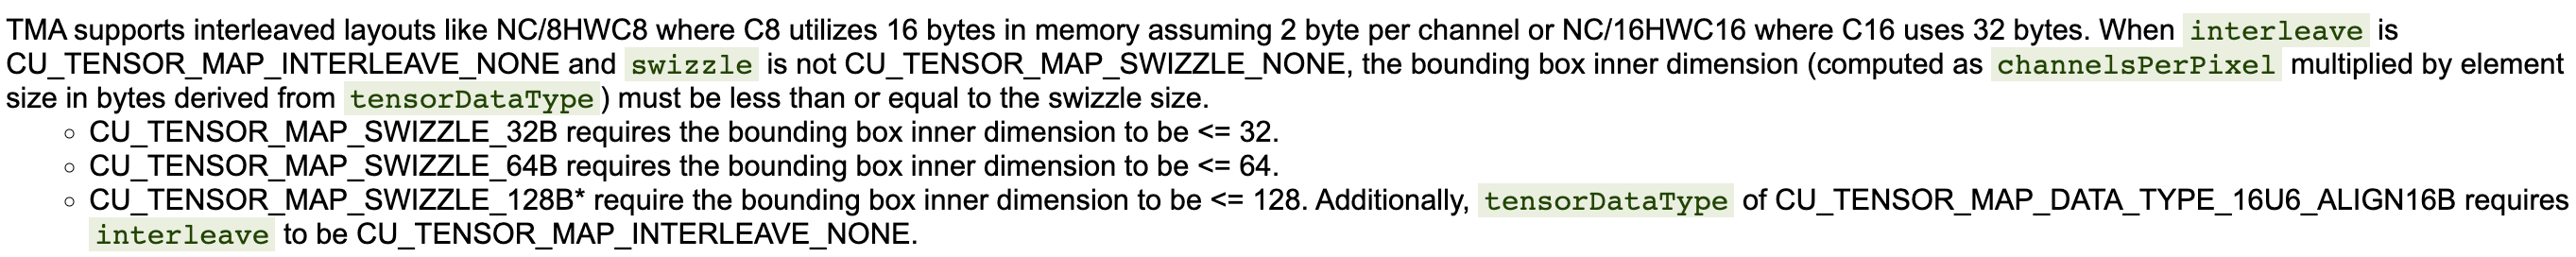
\includegraphics[width=0.9\textwidth]{figures/zhuxi-05-tma-copy/fig-04.png}
\end{figure}

这个限制会体现在 SMEM Layout 上，并由此传递给了 make\_tma\_copy() 函数，最终生成了符合硬件约束的最优 Box Size。

TMA 除了可以做到简单的数据 copy，还可以做到一次 load 数据写出到多个 SM 上的 shared mem 上（要求这些 SM 在同一个 cluster 上）。例如，我们在 gemm kernel 这类存在数据复用的场景，可以做到一个 TileA 广播给 SM0 和 SM1 使用，这样对于 SM0 和 SM1 来说，只需要各自读取 1/2 TileA 的数据并 multicast 给对方，就可以正常完成后续的 gemm 操作了，能大大减少 load 的数据量，是一个非常实用的功能。

在 CuTe 中，其做法就是将 TileA 的上半部分交给 SM0 copy，TileA 的下半部分交给 SM1 copy。这时候虽然 SM0 和 SM1 的 tma 各自只 load 了 1/2 TileA 数据，但是每个 SM 都收到了 TileA 的数据量，所以我们设置 transaction bytes 也仍然是完整 TileA 的量，原则就是每个 sm 并不关心自己的 TMA 发了多少数据的 copy，只管自己接收到了多少数据。

读者可能有疑问，为什么不直接拆分为左右各一条 tma copy 然后 multicast？我猜测这里是为了通用性考虑，因为 tile size 可能是 64 的奇数倍，例如 192，这时候如果做左右拆分，会有一条 copy 指令只有一个 SM 在做，另一个 SM 在等待，且不说性能会不如均分（max(2, 1) $>$ mean(2, 1)），可维护性也是个大问题。

我们可以将上述 make\_tma\_copy 描述过程展示如 Fig.4。

\begin{figure}[htbp]\centering

\includegraphics[width=0.9\textwidth]{figures/zhuxi-05-tma-copy/fig-05.jpg}
\caption{Figure 4. make\_tma\_copy() 执行流程。包含贪心合并 TMA 维度，descriptor 的生成，multicast 处理等流程，得到最优的 copy 方案。}
\end{figure}

在上述的介绍中，我们提到 \textbf{fill\_tma\_gmem\_shape\_stride()} 这个函数会对超过 5D 的数据进行压缩，在此我们给读者朋友一个挑战：

尝试思考一下其是如何做这个压缩的（为什么用到 GCD 最大公约数），这个压缩并不完美，其潜在问题是什么。如果读者对这个部分也能思考清楚，可以认为你对 TMA 有了相当清楚的认知，我们在评论区给出答案，也欢迎大家给出自己的看法。

\section{TMA proxy \& fence}

通过 TMA 来 load / store shared mem，和正常 sts 以及 lds 指令访问 shared mem 所走的数据通路（后者走 Load Store Unit, LSU）是不同的，但是其访问的数据又有可能是同一段地址。这时两个访问方式就被称为两个 Proxy：正常走 LSU 的 proxy 被称为 \textbf{Generic Proxy}，TMA 走的 proxy 被称为 \textbf{Async Proxy}。

不同 proxy 访问同一块地址会出现内存可见性的问题，因为硬件之间无法即时同步这个地址的读写状态，因此要加一个 \textbf{fence} 来保障跨 Proxy 的内存可见性。

例如，在 GEMM Kernel 中，通常在计算完成需要输出结果到 Global Memory 时，会先从 Register Copy 到 Shared Mem 中（不管调用的是 stmatrix 还是 sts 指令，其对应的硬件单元都是 LSU），然后再经由 TMA 发起从 Shared Mem 到 Global Mem 的 Copy。这里为了保证 TMA 搬运的数据是 LSU 刚刚写入的最新的数据，必须要在两者之间加一个 TMA Fence，其指向的 ptx 代码如下：

\begin{lstlisting}[language=C++]
// Issue a shared memory fence for async operations
CUTLASS_DEVICE
void fence_view_async_shared() {
#if CUDA_BARRIER_ENABLED
    cutlass::arch::synclog_emit_fence_view_async_shared(__LINE__);
    asm volatile (
        "{\n\t"
        "fence.proxy.async.shared::cta; \n"
        "}"
        ::
        : "memory");
#else
    CUTLASS_NOT_IMPLEMENTED();
#endif
}
\end{lstlisting}

这里值得注意的是，\textbf{fence 和 sync (\_\_syncthreads 或是 named barrier sync) 是两个不同维度的原语}。

\verb|__syncthreads| 仅保证了 Generic Proxy 下的线程同步和内存一致性（即，确保所有线程都已经把数据写进 shared mem），但它\textbf{并不保证}跨 Proxy 的可见性。 因此，如果只做 sync 不做 fence，TMA 单元可能看不到 LSU 刚刚写入的数据；反之，如果只做 Fence 不做 Sync，TMA 发起时可能其他线程还没写完数据。

所以，正确的流程通常是：先 \textbf{sync}（确保数据就绪），再 \textbf{fence}（确保 TMA 可见），最后发起 \textbf{TMA Store}。那么 sync 的时候为什么不把 fence 一起做了呢？因为这个操作只有在涉及跨 Proxy（如 STS 和 TMA 混用）的特定场景下才需要。如果在所有 sync 中都强制加入 fence，在大量不需要跨 Proxy 交互的场景下（例如纯 CUDA Core 计算）会引入不必要的开销，得不偿失。

\section{总结}

本文介绍了从 Hopper 架构开始引入的 \textbf{Tensor Memory Accelerator (TMA)，其出现是为了充分利用 GPU 越来越高的 IO 带宽，确保 IO bound 和 Compute bound kernel 都能达到预期性能。}具体的，其实现了仅需一条指令即可将整块 Tile 搬运至 Shared Memory，从而释放了带宽潜力。

然而，代价是什么？

TMA 的出现深刻改变了 GPU 的编程范式，并引入了一系列新概念，如 descriptor，barrier，proxy 等等，对于一个从 Ampere 架构下切换过来的开发者来说是一个不小的心智负担。

好在我们可以借助 \textbf{CuTe} 来驾驭这一硬件特性。因此，我们在本文中重点介绍了\textbf{ CuTe 坐标体系}，\textbf{MBarrier 的 Phase 翻转机制}，并重点解读了 \textbf{make\_tma\_copy 函数}，其能够针对硬件的维度限制和 Box Size 限制进行贪心的维度合并来最大化带宽，并能够很好的处理 multicast 场景。最后我们讨论了保证 Generic/Async Proxy 内存可见性的 \textbf{fence} 机制，确保写出的 kernel 的数据正确性。

笔者的一个感受就是，CuTe 的核心代码确实难读，但是好处是其经过开源的检验，并有 CUTLASS / Flash Atten 这样可以借鉴的高质量代码库。笔者曾经参与维护过一套手写 PTX 搭建的 TMA + WGMMA 类算子，在叠加上各种异步优化之后代码变得非常难维护，经常发现查了一天 bug 发现是某行有个坐标算错了，或是某个 barrier 没同步好。

人的智慧应当用于构建更宏大的系统，而非消耗在底层的比特泥沼之中。\textbf{“君子生非异也，善假于物也。”} 愿诸君善用利器，从繁琐的指令细节中解放出来，去追求更具价值的架构创新。\textbf{Save code, live long。 }

\chapter{写给进阶开发的 CuTe 笔记：tiled mma 的 permutationMNK 参数}

\begin{center}\small 作者：竹熙佳处（知乎专栏「CuTe 教程」）\quad 原文：\url{https://zhuanlan.zhihu.com/p/1973526710105419953}\end{center}

\section{前言}

在之前的写给大家看的 CuTe 教程：tiled mma\footnote{\url{https://zhuanlan.zhihu.com/p/1937145378446226159}}[1]文章中，我们介绍了 permutation MNK （以下记作 PermMNK）作为 tiler 的作用，但是并没有介绍其真正 “permutation” 的功能。

在文章中我们提到，在 cutlass repo 的 issue: What is PermutationMNK in TiledMMA in CUTLASS 3.4 changes?\footnote{\url{https://link.zhihu.com/?target=https\%3A//github.com/NVIDIA/cutlass/discussions/1345}} [2] 中，CuTe 的作者 Cris Cecka\footnote{\url{https://link.zhihu.com/?target=https\%3A//github.com/ccecka}} 进行了解答，其可以做到让每个 thread 做 mma 时可以更灵活的指定自己所负责的数据。但是笔者觉得，其介绍仍然延续了 CuTe 官方文档类似的问题：缺少足够的上下文以及一步步 reasoning 的过程，导致理解起来仍然非常不直观。在本文中，我们尝试用更直白的语言，帮助读者一同理解这个参数的含义以及用法。

值得注意的是，虽然 permutation 的功能在绝大多数使用 CuTe 的场景下都用不到，但是其在一些特殊场景下可能能有奇效。因此本系列文章主要面向 cute 进阶开发者收录于写给进阶开发者的 CuTe 教程\footnote{\url{https://zhuanlan.zhihu.com/column/c_1973695125898150444}}[3]，作为 写给大家看的 cute 专栏\footnote{\url{https://zhuanlan.zhihu.com/column/c_1946580149119202264}} [4]的补充，主要用来解释 CuTe 中不易理解但具有潜力的细节。读者朋友们有感兴趣的内容可以在评论区提出，我们在后续的文章中进行选择梳理。

\section{动机}

我们以 ampere-style fp16 mma 为例，考虑一个场景：一个 warp 完成 2 次 16x8x16 的 mma，得到 16x16 的 C，然后 store 到 global mem。在一些场景下，例如 M \& N 很大，K 很小的场景下，这时候 STG 指令的发射可能构成瓶颈，因此我们希望 store 的时候，用到更大字长的 STG，如 STG.128 来提升 store 的效率。

但是如我们在 tiled mma 篇章中介绍的，mma 指令决定了我们的 thread 存放的数据最多只能写出连续的两个 value，如 Fig.1 所示，如果是 float 数值，最大能用的 STG 指令只能是 STG.64。

\begin{figure}[htbp]\centering

\includegraphics[width=0.9\textwidth]{figures/zhuxi-06-permmnk/fig-01.jpg}
\caption{Figure.1 16x8x16 FP16 mma 指令 C 矩阵对应的 thread-value 映射关系。可以看到每个 thread 会得到 C 矩阵中特定位置的数据}
\end{figure}

这时候，我们希望 thread0 要是能得到 C 矩阵中的连续的 4 个 value 就好了。这其实就是 permutationMNK 被提出的动机。类似的情况还包含 w4a8 混合精度 gemm，fp8 attention（QK 乘之后的 P 矩阵作为 fp8 mma 输入，需要 4 个数连续），也可以尝试用这个方法。

\section{如何使用 PermMNK}

在 issue [2] 中，Cris Cecka\footnote{\url{https://link.zhihu.com/?target=https\%3A//github.com/ccecka}}以 fp64 mma 来作为实例以方便可视化，与上述我们给的例子本质是一样的。为展示方便，我们仍然以其在该 issue 中例子上进行分析。首先，在常规的用法中，我们指定 permMNK 为一个普通的 tile 时，对应代码如下：

\begin{lstlisting}[language=C++]
TiledMMA tiled_mma = make_tiled_mma(SM80_8x8x4_F64F64F64F64_TN{},
                                     Layout<Shape<_1,_1,_1>>{},     // AtomLayout
                                     Tile<_8,_16,_8>{});            // Tiler
\end{lstlisting}

我们观察 mma 的执行过程与 thread 中存放 C 的 reg 数据，可以如 Fig.2 所示：

\begin{figure}[htbp]\centering

\includegraphics[width=0.9\textwidth]{figures/zhuxi-06-permmnk/fig-02.jpg}
\caption{figure2. 常规调用 2 次 mma，thread0 拿到的 C 矩阵数据对应坐标为\{(0, 0), (0, 1), (0, 8), (0, 9)\}，无法作为连续的数据写出}
\end{figure}

如我们所预期的，每个 thread 拿到的数据在写出时是不连续的。原因即是我们遵循 mma 的标准做法：对 B 矩阵进行了连续的读取，并做了两次连续的 mma。

但是，如果我们可以\textbf{让两条 mma 指令，不处理 A \& B 矩阵在物理上连续的数据块，而是交错式的取数据，计算的结果也交错写出到 C 矩阵中；然后再执行第二条 mma，依旧是读交错的位置，得到的结果交错写入 C reg 矩阵。}这个过程如 Fig.3 所示：

\begin{figure}[htbp]\centering

\includegraphics[width=0.9\textwidth]{figures/zhuxi-06-permmnk/fig-03.jpg}
\caption{figure2. 交错调用 2 次 mma，thread0 拿到的 C 矩阵数据对应坐标为 \{(0, 0), (0, 1), (0, 2), (0, 3)\}，可以作为连续的数据写出}
\end{figure}

我们发现，通过这样计算出来的 C 矩阵，各个 thead 能够拿到连续的 4 个数，STG.128 就可以执行了！那么这个写法，对应到 permutationMNK 的参数如下，其就是在 N 维度做了重排：

\begin{lstlisting}[language=C++]
TiledMMA tiled_mma = make_tiled_mma(SM80_8x8x4_F64F64F64F64_TN{},
                                     Layout<Shape<_1,_1,_1>>{},     // AtomLayout
                                     Tile<_8,                       // Permutation on M, equivalent to 8:1, identity
                                     Layout<Shape <_2,_4,_2>, 
                                             Stride<_1,_4,_2>>, // Permutation on N, size 16
                                      _8>{});                   // Permutation on K, equivalent to 8:1, identity
\end{lstlisting}

那么再考虑，用于 s2r copy 的 LDSM 指令在这个时候是否还可以使用？笔者认为是可以的，因为虽然我们在 N 方向上有一些交错访问，但是交错的粒度，都是连续的 2*16 fp16 元素，因此 LDSM 仍然可以使用。不过，由于从 shared mem 中 load 的数据不再是紧密排列的了，常规的 swizzle BMS 参数需要重新调整一下才能做到 bank-conflict-free。

进一步的，我们思考，想要完成上述功能，除了 permMNK 之外，原本的 g2s -$>$ s2r -$>$ gemm 的 mainloop 代码还需要做什么改动吗？笔者认为应该是不需要的，我们观察 permMNK 在 tiled mma 的具体实现，其是通过 logical\_divide 改动了 TV-layout，其作用会自然而然通过 partition 和 retile 的逻辑传递到 s2r tiled copy 上。

\begin{lstlisting}[language=C++]
thrfrg_C(CTensor&& ctensor) const
{
  CUTE_STATIC_ASSERT_V(rank(ctensor) >= Int<2>{});
  // Reorder the tensor for the TiledAtom
  auto t_tile = make_tile(permutation_mnk<0>(),
                          permutation_mnk<1>());
  auto t_tensor = logical_divide(ctensor, t_tile);                 // (PermM,PermN)

  // ...
}
\end{lstlisting}

为了验证 "permMNK 修改并不影响 ldmatrix 以及 mainloop 流程" 的想法，我们给出验证代码，有兴趣的读者可以尝试复现：

\url{https://github.com/chrisHuxi/CuTe-coding-toolings/blob/feature/permMNK_tiled_mma/permMNK_example/perm_tiled_mma.cu}

此外，有读者朋友@6666\footnote{\url{https://www.zhihu.com/people/940468f485e92a6af2c696581a440e60}}在评论区也给出了 CuTeDSL 的实现，发现在设置 permMNK 后再调用 ldmatrix 会产生报错，笔者初版判断是 CuTeDSL 本身的适配问题，待我们研究清楚后再更新结论到本文中，有熟悉 CuTeDSL 的读者也欢迎在评论区讨论。

\section{总结}

本文中，我们介绍了 Tiled mma 中 permutationMNK 参数的作用。其通过修改 TV-layout，做到对每个 thread 负责输出 C 矩阵的位置进行微调，从而赋予了 load / store 时更多的灵活性。从这个例子我们可以看到，CuTe 的抽象确实足够完备，但高度的抽象也隐藏了诸多细节，确实不易理解，希望我们的梳理能够帮助大家进一步加深对 CuTe 的理解。

\section{Reference}

[1] 写给大家看的 CuTe 教程：tiled mma\footnote{\url{https://zhuanlan.zhihu.com/p/1937145378446226159}}

[2] [QST] What is PermutationMNK in TiledMMA in CUTLASS 3.4 changes?\footnote{\url{https://link.zhihu.com/?target=https\%3A//github.com/NVIDIA/cutlass/discussions/1345}}

[3] 写给进阶开发看的 CuTe 教程\footnote{\url{https://zhuanlan.zhihu.com/column/c_1973695125898150444}}

[4] 写给大家看的 CuTe 教程\footnote{\url{https://zhuanlan.zhihu.com/column/c_1946580149119202264}}

\chapter{写给大家看的 CuTe 教程：async pipeline}

\begin{center}\small 作者：竹熙佳处（知乎专栏「CuTe 教程」）\quad 原文：\url{https://zhuanlan.zhihu.com/p/2024832248386528275}\quad 抓取：2026-09-20\end{center}

\section{动机}

在之前的文章[1][2]中，我们介绍了 Hopper 架构引入的 TMA 来提升数据搬运的能力。TMA 让我们能以一条指令搬运一整块 Tile 数据到 Shared Memory，mbarrier 则提供了约束异步操作的顺序的能力。

由于本文介绍的 async pipeline 围绕 mbarrier 构成，我们首先高度精简地回顾一下：

\begin{quote}
mbarrier 是一个 64-bit 的 shared memory 变量，内部包含 phase、expect arrival count、expect transaction bytes 等字段。当实际的 arrival count 和 transaction bytes 都达到预期值时，phase 位翻转，正在 wait 这个 barrier 的操作即可继续执行。更多细节的可以参考:
\end{quote}

写给大家看的 CuTe 教程：TMA Copy

构建于 TMA \& mbarrier 两大设计之上，针对 gemm / attention 这类 tensor core kernel，NVIDIA 在 Hopper 架构中推出了 Warp Specialization 编程范式，并在后续架构延续下来。以 gemm 为例来说明：

\begin{itemize}
  \item 让一小部分 Warp 专门做 Producer，只负责向 TMA 发送搬运指令，写 A/B tile 数据到 Shared Memory；
  \item 让绝大部分 Warp 专门做 Consumer，只负责从 Shared Memory 读数据做 mma。
\end{itemize}

Producer 和 Consumer 各自独立运行，天然就具备了数据搬运与计算的重叠能力，同时也大大简化了编译器优化的压力。然而，这也引入了一个新问题：两者之间如何协调？ 具体地，我们需要解决两个问题：

\begin{itemize}
  \item \textbf{Consumer 怎么知道数据已经 ready 了？}—— 不能在 Producer 还没搬完的时候就去读 Shared Memory。
  \item \textbf{Producer 怎么知道旧数据已经被用完了？}—— 不能在 Consumer 还在读 Shared Memory 的时候就覆盖写入下一轮数据。
\end{itemize}

如果只有一块 Shared Memory Buffer，那 Producer 搬完就得等 Consumer 算完，Consumer 算完又得等 Producer 搬下一轮，成为了串行模式，自然不是高效的。

因此，我们引入 multi-stage，即，准备多块（如，3 块） Shared Memory Buffer，生产者往 Stage 1 写数据的同时，消费者可以从 Stage 0 的 shared mem 读上一轮的数据，两者在不同的 Stage 上交替工作，形成 load 数据以及计算的 overlap。即，我们需要维护一个stage-id 从  0 -$>$ 1 -$>$ 2 -$>$ 0 -$>$ …  的环形 buffer，我们在每一次 stage-id 变化时及时 arrive barrier，以让依赖这个 buffer 的 warp 可以解除 wait，继续执行。

朴素地，我们可以手动地维护 stage-id 的循环逻辑与 barrier 的状态，但是真正写过复杂 tensor core kernel 的读者，大概会发现，这不是一个好的选择，一个不留神就容易 hang 住，或是 arrive 时机不对导致报错或是结果异常。因此，我们可以构建一个结构体来管理 barrier 以及 multi-stage 的状态、协调生产者和消费者在各个 Stage 上的访问权限，此即 AsyncPipeline。

此外，AsyncPipeline 的适用范围不限于 TMA + MMA。MMA + Epilogue、Pingpong MMA 等场景同样可以用 Pipeline 来做交互，只要存在异步的 “生产” 和 “消费” 关系，AsyncPipeline 都能派上用场，因此我们在完成复杂 tensor core kernel（尤其是 sm100，引入了 umma 以及 tensor memory 后，tma -$>$ umma -$>$ tmem -$>$ epilogue 这套流程需要维护的异步状态变得异常烧脑，更不要说 flash atten v4 这样引入 softmax + 两次 umma 的用法），AsyncPipeline 就更是不可或缺的基础组件。

因此，在本文接下来的内容中，我们结合 cutlass 中的具体实现，来了解其用法以及不可绕过的实现细节。

\section{基本用法}

我们首先来看一个简单的例子，借助其经典用法下 TMA + MMA，来了解 \textbf{AsyncPipeline 的基本用法}，然后逐一梳理各细节。

\begin{lstlisting}[language=C++]
// ===== 初始化 =====
PipelineTmaAsync pipeline(shared_storage, params);
PipelineState pipe_read;   
PipelineState pipe_write; 

  // --- 生产者：搬数据 ---
  if (is_producer) {
    pipeline.producer_acquire(pipe_write);          // wait EmptyBarrier
    copy(tma_load.with(full_barrier(pipe_write)));  // issue tma copy
    ++pipe_write;                                   // advance to next stage
  }

  // --- 消费者：算数据 ---
  if (is_consumer) {
    pipeline.consumer_wait(pipe_read);               // wait FullBarrier
    gemm(acc, smem_A, smem_B);                       // issue mma
    pipeline.consumer_release(pipe_read);            // arrive EmptyBarrier
    ++pipe_read;                                     // advance to next stage
  }
\end{lstlisting}

\section{AsyncPipeline：mbarrier 的封装}

Async Pipeline 本质上是一个封装了 mbarrier 的结构体，并提供了对 barrier 操作的各项接口。那么，我们来推导一下这个结构体需要什么成员变量以及函数。首先我们思考，在 TMA + MMA 场景下，我们应该用多少个 mbarrier 来确保数据的使用不重不漏呢？

答案是：每个 Stage 都配备一对 barrier，分别用来约束：

\begin{itemize}
  \item MMA warp 在此等待，直到 “TMA 已经 load 完数据到 buffer 了，MMA 可以使用了”，我们记为\textbf{ full barrier；}
  \item TMA warp 在此等待，直到 “MMA 已经使用完 buffer 里的数据了，TMA 可以 load 下一轮数据了”，记为 \textbf{empty barrier。}
\end{itemize}

所以，我们可以看到，Pipeline 的成员变量 \verb|SharedStorage| 结构体如下：

\begin{lstlisting}[language=C++]
struct SharedStorage {
  FullBarrier  full_barrier_[Stages];
  EmptyBarrier empty_barrier_[Stages];
}
\end{lstlisting}

除了 barrier 变量本身，这个结构体还提供对 barrier 操作的一系列函数，包括：

\begin{lstlisting}[language=C++]
void producer_acquire(state); 
// producer 等待当前 state 的 empty barrier 就位

void producer_commit(state);
// producer 在发出当前 state 的数据生产任务后 arrive 对应的 full barrier，TMA load 场景下为 NOP

void consumer_wait(state);
// consumer 等待当前 state 的 full barrier 就位

void consumer_release(state);
// consumer 在发出当前 state 的数据消费后 arrive 对应的 empty barrier
\end{lstlisting}

我们逐个说明：

\begin{itemize}
  \item \textbf{producer\_acquire(state)}：\textbf{producer 等待当前 state 的 empty barrier 就位}，即，其在等待 consumer 将当前 stage 的 shared mem buffer 使用完毕。
  \item \textbf{producer\_commit(state)}：\textbf{producer 在发出当前 state 的数据生产任务后 arrive 对应的 full barrier}。这一步在 TMA load 场景下是不需要的（当然写了也没事，会被编译为一个 NOP 操作），因为 TMA load 的 arrive 在 \verb|copy()| 函数中就已经提交了；但在如 umma + load tmem 这类 pipeline 场景下则是必要的。
  \item \textbf{consumer\_wait(state)}：\textbf{consumer 等待当前 state 的 full barrier 就位}，即，等待 producer 将当前 stage 的 shared mem buffer 填满。
  \item \textbf{consumer\_release(state)}：\textbf{consumer 在发出当前 state 的数据消费后 arrive 对应的 empty barrier。}
\end{itemize}

有了这 4 个函数，我们实际上再回头来看我们的代码，就很清晰了。语义上，每个 warp 每次都是 acquire 到需要的资源之后，就开始执行（copy/gemm），执行完成后 release 当前的资源。

我们可以借助 Fig.1 来理解这个过程中是如何使用 AsyncPipeline的：

\begin{figure}[htbp]\centering

\includegraphics[width=0.9\textwidth]{figures/zhuxi-07-async-pipeline/fig-01.jpg}
\caption{Figure 1. Producer 与 Consumer 通过 AsyncPipline 交互示意图；每个 Stage 都配备一对 barrier，full \& empty，分别用来表示 tma 已经填满当前 stage 的 shared mem buffer \& mma 已经使用完当前 stage 的 shared mem buffer}
\end{figure}

此外，由于一些指令如 tma copy，是由单 thread 发起的，而如 epilogue 或是 softmax 这样的指令，仍然由多条 thread 共同完成。

这涉及到我们对 mbarrier 初始化，以及实际 arrive 的时候区别对待（即，arrive 一次还是多次），因此这就要求我们的 pipeline 带有身份信息，例如， “当前 warp 是 producer 还是 consumer？” 或是“这个 thread 是用来发射 TMA 指令的 leader thread 吗？” 。那么这段身份标识，就需要在 Pipeline 初始化的时候以 param 的方式传递给 pipeline 结构体。其核心代码可以展示为如下：

\begin{lstlisting}[language=C++]
enum class ThreadCategory {
    NonParticipant,
    Producer,
    Consumer,
    ProducerConsumer
  };

  struct Params {
    uint32_t transaction_bytes = 0;
    ThreadCategory role = ThreadCategory::NonParticipant;
    uint32_t is_leader = 0;
    uint32_t num_consumers = 0; // Number of consumer threads
    uint32_t num_producers = 1; // Number of producer threads
    int initializing_warp = 0; 
  };
  
// PipelineTmaAsync constructor
  template<class ClusterShape, class InitBarriers, class InitMasks>
  CUTLASS_DEVICE
  PipelineTmaAsync(SharedStorage& storage, Params params, ClusterShape cluster_shape, InitBarriers = {}, InitMasks = {})
      : params_(params)
      , full_barrier_ptr_(&storage.full_barrier_[0])
      , empty_barrier_ptr_(&storage.empty_barrier_[0]) {
      // ...
  }
\end{lstlisting}

\section{PipelineState：流水线的状态机}

我们观察到，pipeline 结构体提供了对 mbarrier 的各种操作，但在 multi-stage 下，我们仍然需要手动映射当前的 i-k-tile、i-stage 以及预期的 barrier 状态，实际上仍然是比较烧脑的。笔者曾经因为历史原因维护过一套不借助 cutlass 的函数写的 sm90 flash atten 算子，各种 barrier 状态的转移分析和 debug 真是遭老罪了。

因此，CuTe 中提供了一个新的结构体来完成状态的管理：\verb|PipelineState|。其核心定义如下：

\begin{lstlisting}[language=C++]
// Circular Buffer Index + Associated Phase
// Assumes only one operation possible - i.e., ++
template<uint32_t Stages_>
struct PipelineState {
  static constexpr uint32_t Stages = Stages_;

  int index_ = 0;
  uint32_t phase_ = 0;
  uint32_t count_ = 0;

  CUTLASS_DEVICE
  PipelineState(int index, uint32_t phase, uint32_t count)
    : index_(index)
    , phase_(phase)
    , count_(count) {}

  CUTLASS_DEVICE
  void operator++() {
    if constexpr (Stages > 0) {
      ++index_;
      ++count_;
      if (index_ == Stages) {
        index_ = 0;
        phase_ ^= 1;
      }
    }
  }
}
\end{lstlisting}

具体来说，PipelineState 只是维护了三个变量：

\begin{itemize}
  \item count\_：自流水线启动以来，总共经历的 k-tile id，这个值是一直增长的。
  \item index\_：当前 stage 的 id，如在 3-stage 设定下，其就是 0-$>$1-$>$2-$>$0-$>$1 … 的循环。
  \item phase\_：当前 k-tile 下，我们等待的 mbarrier phase，只有 0 和 1 两个取值。若为 1，只有在 mbarrier phase 也会 1 的时候进行阻塞，mbarrier phase 为 0 的时候放行；反之则反。
\end{itemize}

index\_ 和 count\_ 的语义是较平凡的，关键在于 phase\_。我们用一个 3-Stage 的 producer\_state 的例子，随着 k-tile 的递增，来观察它们的变化规律。

这里我们需要提一下一个细节（感谢读者朋友 @最光阴\footnote{\url{https://www.zhihu.com/people/7bb7911bb19edeb4bacade3815513a47}} 的提醒），由于 empty barrier 在初始化时，phase 位为 0，而，而我们第一次发起 TMA 时，shared mem buffer 都是空的，也就是不需要阻塞，所以我们会将 producer\_state 的状态初始化为 \{ index\_ == 0, phase\_ == 1, count\_ == 0 \}，否则 Producer 会等待一个无法解锁的 empty barrier，一上来就 hang 住。这个phase\_ == 1在 prodcuer\_state 上是必要的，在 consumer\_state 中则不必要。

我们将时间线展开如 Fig.2 所示：

\begin{figure}[htbp]\centering

\includegraphics[width=0.9\textwidth]{figures/zhuxi-07-async-pipeline/fig-02.jpg}
\caption{Figure 2. Producer 与 Consumer 在 k-tile 循环过程 \& producer\_state 中各变量变化情况；index 指向 stage-id，0,1,2,0,1,2 循环，count 随着 k-tile 进行不断递增，phase 则是每 3 次翻转一次。第一次发起 TMA 时，不需要阻塞，所以我们会将 producer\_state 的 phase\_ 初始化为 1}
\end{figure}

可以看到，从 0 开始，在每次完成 3 次 k-tile 后（即，所有 stage 的 shared mem buffer 都被用到了），phase\_ 会发生一次位翻转(0-$>$1 或是 1-$>$0)，这实际上代表着我们预期当前的 mbarrier 的状态应该发生了变化。因为在 multi-stage-buffer 场景下，同一个 stage 会被反复使用（第 0 轮用 stage 0，第 3 轮又轮到 stage 0），如果没有 phase 状态的标记，硬件就无法区分 "这是新一轮的通知" 还是 "上一轮留下来的残余状态"。

phase 的巧妙之处在于，它让 barrier 的状态具备了代际区分能力，而无需在每轮开始前显式清理 barrier—— 硬件自动通过 phase 比对完成这一切。只有当 mbarrier 本身的 phase 位和我们在 PipelineState 里的这个需要等待的 phase\_ 不一致时，wait 之后的代码才能被放行。因此，通过这样一个结构体，我们就能很轻松的完成 multi-stage 下 mbarrier 状态的管理。

\section{总结}

Mbarrier 的引入，正式将 CuTe kernel 转变为 warp-specialized + producer \& consumer 范式，然而多个 producer \& consumer 的设定，叠加 multi-stage buffer，让 mbarrier 的状态维护变得极为复杂。

为了解决这个问题，cutlass 提供了 AsyncPipeline 结构体，提供了对 full\_barrier 和 empty\_barrier 操作的封装。

进一步地，我们在使用 AsyncPipeline 时，通常会同时再为 producer \& consumer 分别定义一个 PipelineState，用以管理 k-tile \& i-stage \& 预期的 phase 三者的映射关系。

具体来说，我们只需在每次循环后将 PipelineState 作为参数传给 AsyncPipeline 的对应函数（acquire/commit/release），在每次循环结束前 ++PipelineState，就能让维护状态的复杂度在封装好的函数中消化掉。

至此，我们已经梳理完 CuTe 中写好一个 tensor core kernel 所需的基本概念，包括 tiled\_copy[3]，tiled\_mma[4]，tma\_copy[1] 以及 async\_pipeline，因此接下来的文章，我们来尝试用这些组件搭建一个 SOTA 级别的 kernel（e.g gemm / attention @ RTX5080）。


\end{document}
